\documentclass[12pt]{article}  

\usepackage[boxruled,lined]{algorithm2e}
%% \usepackage{booktabs}
\usepackage{amsmath} 
\usepackage{amsthm} 
\usepackage{amsfonts} 
\usepackage{enumitem}
\usepackage[T1]{fontenc}
\usepackage[utf8]{inputenc}
\usepackage{xparse} 
\usepackage{bm}
\usepackage{bbm} 
\usepackage{color,soul} 
\usepackage{framed}
\usepackage[margin=0.5in]{geometry}
\usepackage{gensymb}
\usepackage{hyperref}
\usepackage{mathtools}
\usepackage{multicol}
\usepackage[dvipsnames]{xcolor}
\usepackage{tikz}
\usepackage[normalem]{ulem}
\usepackage{pgfplots}  
\usepackage{pifont}
\usepackage{colortbl}
\usetikzlibrary{positioning}
\usetikzlibrary{calc}
\usetikzlibrary{fit}
\usetikzlibrary{shapes}
\usetikzlibrary{patterns}
\usetikzlibrary{decorations.pathreplacing}
\newcommand\STAR{{\tikz{\node[draw,star,star point height=.7em,minimum size=1em,scale=0.35]{};} }}
\newcommand{\Plus}{\mathord{\begin{tikzpicture}[baseline=0ex, line width=1, scale=0.13]
\draw (1,0) -- (1,2); \draw (0,1) -- (2,1); \end{tikzpicture}}}

\newtheorem{theorem}{Theorem}[section]
\newtheorem{lemma}[theorem]{Lemma}
\newtheorem{proposition}[theorem]{Proposition}
\newtheorem{corollary}[theorem]{Corollary}
\DeclarePairedDelimiter{\ceil}{\lceil}{\rceil}
\DeclarePairedDelimiter{\floor}{\lfloor}{\rfloor}
\DeclareMathOperator*{\argmin}{arg\,min}
\DeclareMathOperator*{\argmax}{arg\,max}
\newcommand{\D}{\mathrm{d}}
\SetKwInput{KwInput}{Input}
\SetKwInput{KwOutput}{Output}

\definecolor{deepblue}{rgb}{0,0,0.5}
\definecolor{deepred}{rgb}{0.6,0,0}
\definecolor{deepgreen}{rgb}{0,0.5,0}

\def\foldedpaper#1{
    \tikz[scale=#1,line width={#1*1pt}]{
        \def\a{1.41} % relative height
        \def\b{0.2}  % relative height/width of corner
        \def\c{0.1}  % relative margin width (on either side)
        \def\d{0.05} % vertical offset of lines
        \def\N{6}    % number of lines
        \draw         (0,0)
                --  ++(-1,0)
                --  ++(0,\a)
                --  ++(1-\b,0)
                --  ++(\b,-\b)
                -- cycle;
        \foreach \lnum in {1,...,\N}{
            \pgfmathsetmacro\yline{\a-\d-\lnum*\a/(\N+1)}
            \draw (-1+\c,\yline) -- (-\c,\yline);
        }
        \draw[fill=white] (0,\a-\b) -- ++(-\b,0) -- ++ (0,\b);
    }
}

\usepackage{listings}

% Default fixed font does not support bold face
\DeclareFixedFont{\ttb}{T1}{txtt}{bx}{n}{12} % for bold
\DeclareFixedFont{\ttm}{T1}{txtt}{m}{n}{12}  % for normal
% Python style for highlighting
\newcommand\pythonstyle{\lstset{
language=Python,
basicstyle=\ttm,
otherkeywords={self,for,range,in,True,yield},             % Add keywords here
keywordstyle=\ttb\color{deepgreen},
emph={MyClass,__init__},          % Custom highlighting
emphstyle=\ttb\color{deepred},    % Custom highlighting style
stringstyle=\color{deepgreen},
frame=tb,                         % Any extra options here
showstringspaces=false            %
}}


% Python environment
\lstnewenvironment{python}[1][]
{
\pythonstyle
\lstset{#1}
}
{}

% Python for external files
\newcommand\pythonexternal[2][]{{
\pythonstyle
\lstinputlisting[#1]{#2}}}

% Python for inline
\newcommand\pythoninline[1]{{\pythonstyle\lstinline!#1!}}


\usetikzlibrary{shapes.misc}
\usetikzlibrary{shapes.arrows}

\tikzset{cross/.style={cross out, draw=black, minimum size=2*(#1-\pgflinewidth), inner sep=0pt, outer sep=0pt},
%default radius will be 1pt. 
cross/.default={2pt}}

\begin{document}
\renewcommand{\d}[1]{\ensuremath{\operatorname{d}\!{#1}}}

\tableofcontents
\newpage
\section{Sentiment Analysis with Logistic Regression}\vspace{.1pt} \hrule height 2pt \smallskip \renewcommand{\arraystretch}{1}% Tighter
\subsection{Intro to Supervised ML and Sentiment Analysis}
In supervised ML, we have input features $X$ and a set of labels $Y$. To get the most accurate predictions, we try to minimize our \emph{error rates} or \emph{cost function} as much as possible: to do this, we'll run our prediction function which takes in parameters $\theta$ to map you input features to output labels $\hat Y$. The best mapping is achieved when the difference between the expected values $Y$ and the predicted values $\hat Y$ is minimized, which the cost function does by comparing how closely your output $\hat Y$ is to your label $Y$. You can then update your parameters and repeat the whole process until your cost is minimized.

\begin{figure}[h]
\begin{center}
  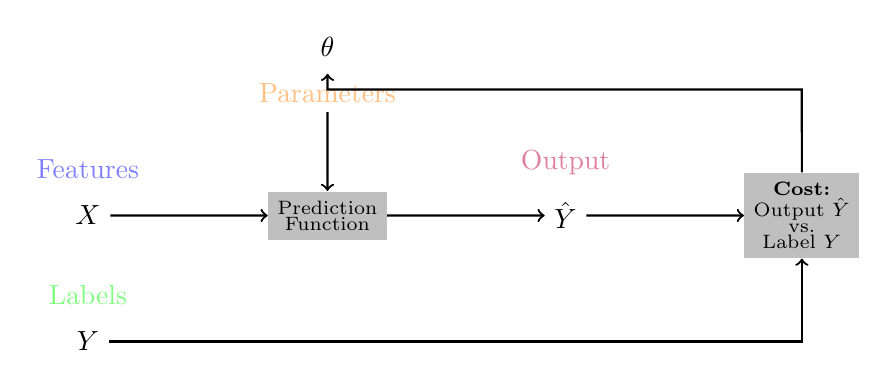
\begin{tikzpicture}[scale=0.8]
    \node (x) at (0, 2) {$X$};
    \node (features) [above=1mm of x] {\color{blue!50}{Features}};
    \node (y) at (0, 0) {$Y$};
    \node (labels) [above=1mm of y] {\color{green!50}{Labels}};
    \node[fill=gray!50,rectangle,right = 2cm of x] (predictionfunction)     {$\substack{\textrm{Prediction} \\ \textrm{Function}}$};
    \node[above = 1cm of predictionfunction] (params)     {\color{orange!50}{Parameters}};
    \node[above = 1mm of params] (theta) {$\theta$};
    \node[right = 2cm of predictionfunction] (yhat) {$\hat Y$};
    \node (output) [above=1mm of yhat] {\color{purple!50}{Output}};
    \node[fill=gray!50,rectangle,right = 2cm of yhat] (cost) {$\substack{\textrm{\textbf{Cost:}} \\ \textrm{Output } \hat Y \\ \textrm{vs.}     \\ \textrm{Label } Y}$};
\draw[->,thick] (x) -- (predictionfunction);
\draw[->,thick] (predictionfunction) -- (yhat);
\draw[->,thick] (yhat) -- (cost);
% Draw a path in two steps and go via a coordinate relative to the first node.
\draw[->,thick] (y) -- node {} ++(2cm,0) -| (cost);
\draw[->,thick] (cost) -- node{} ++(0,2cm) -| (params);
\draw[->,thick] (params) -- (predictionfunction);
\end{tikzpicture}
\end{center}
\label{fig: supervised_ml}
\caption{Overview of supervised machine learning.}
\end{figure}

How about the supervised ML classification task of sentiment analysis? Suppose we're given a tweet that says, ``I'm happy because I'm learning NLP'': and the objective in the task is to predict whether a tweet has a positive or negative sentiment. We'll do this by starting with a training set where tweets with a positive label have a label of unit value, and tweets with a negative sentiment have a label of zero.
To get started building a logistic regression classifier that's capable of predicting sentiments of an arbitrary tweet, we first need to process the raw tweets in our training data set and extract useful features. Then, we will train our logistic regression classifier while minimimizing the cost. Finally, we'll be able to make predictions.

\subsubsection{Representation of Text}
\paragraph{How to represent text as a vector} In order to represent text as a vector, we need to first build a vocabulary. We define the vocabulary $V$ as the \emph{set} of unique words from your input data (e.g. your listing of tweets). To get this listing, we quite literally need to comb through all words from all input data and save every new word that appears in our search.
To represent a tweet as a vector, we can use a one-hot encoding with our vocabulary: i.e. each tweet will be represented with a length $|V|$ vector where elements are binary-valued - a one indicates the word is in the tweet and a zero indicates the absence of a word in a tweet. We call this a \emph{sparse} representation because the number of non-zero entries is relatively small when compared with the number of zero entries. Realize that if we are running a logistic regression, we would require learning $|V| + 1$ parameters which can be problematic for large vocabularies. If not prohibitive, it would make training models take excessive time and making predictions would be expensive.

\paragraph{Negative and positive frequencies} Let's discuss how to generate counts which can be used as features in our logistic regression classifier. Specifically, given a word, we wish to keep track of the number of times that it shows up as the positive class. Given another word, we wish to track how many times that word shows up in the negative class. Using both these counts, we can then extract features and use those features in our logistic regression classifier. Suppose we have the following corpus of tweets:
\begin{verbatim}
I am happy because I am learning NLP
I am happy
I am sad, I am not learning NLP
I am sad
\end{verbatim}
Then our vocabulary is given by
\begin{center}
  \begin{tabular}{c}
    \hline
    Vocabulary \\
    \hline
    I \\
    am \\
    happy \\
    because \\
    learning \\
    NLP \\
    sad \\
    not
  \end{tabular}
\end{center}

For this particular example of sentiment analysis, we only have two sentiments (i.e. two classes): one class is associated with a positive sentiment and the other with a negative sentiment. So, taking your corpus, you'd have a set of two tweets that belong to the positive class, and two tweets which belong to the negative class. Let's calculate the positive frequencies by examining the first two tweets:

\begin{center}
  \begin{tabular}{c c}
    \hline
    Vocabulary & PosFreq(1) \\
    \hline
    I  & 3 \\
    am & 3 \\
    happy & 2 \\
    because & 1 \\
    learning & 1 \\
    NLP & 1 \\
    sad & 0 \\
    not & 0
  \end{tabular}
\end{center}

The same logic applies applies to getting negative frequencies. We can calculate these by examining our last two training examples.


\begin{center}
  \begin{tabular}{c c}
    \hline
    Vocabulary & NegFreq(0) \\
    \hline
    I  & 3 \\
    am & 3 \\
    happy & 0 \\
    because & 0 \\
    learning & 1 \\
    NLP & 1 \\
    sad & 2 \\
    not & 1
  \end{tabular}
\end{center}

So, we can now have an entire table for our corpus, where for each entry in $V$ we associate with it a scalar value \texttt{PosFreq(1)} and another scalar value \texttt{NegFreq(0)}. In practice, we use a Python dictionary \texttt{freqs} mapping from \texttt{(word, class)} $\leadsto$ frequency.

\subsubsection{Feature Extraction with Frequencies} Whereas we previously learned to encode a tweet as a vector of length $|V|$, we will now use our frequency counts to represent each tweet as a vector of length equal to one plus the number of classes in our set of labels. This gives us a much faster speed for our logistic regression classifier. How can we do this, exactly? We represent each tweet as follows:

\begin{align*}
\underbrace{X_m}_{\substack{\textrm{Features of} \\ \textrm{tweet } m}} = \bigg [ \underbrace{1}_{\textrm{Bias}}, \underbrace{\sum_w \texttt{freqs}(w, 1)}_{\substack{\textrm{Sum Pos.} \\ \textrm{Frequences}}}, \underbrace{\sum_w \texttt{freqs}(w, 0)}_{\substack{\textrm{Sum Neg.} \\ \textrm{Frequencies}}} \bigg ]
\end{align*}

I.e. the first feature is a bias unit equal to unit value, the second is the sum of positive frequencies for every unique word on tweet $m$, and the third is the sum of negative frequencies for every unique word on the tweet.
So, to extract the features for this \emph{representation}, we only have to sum frequencies of words, which is straightforward. Let's look at an example: ``I am sad, I am not learning NLP''. The only words in our vocabulary that don't appear in this sentence are ``happy'' and ``because'': if we sum up the \texttt{PosFreq(1)} associated with the remaining words in our vocabulary, i.e. the words that appear in this tweet, we get a scalar value of eight. We do the same for the negative frequencies, and we get a scalar value of eleven. So, we represent ``I am sad, I am not learning NLP'' $\leadsto [1, 8, 11]$.

\subsubsection{Preprocessing} There are two major concepts here: stemming and ``stop words''.
We'll learn how to apply these preprocessing steps to our data.
\paragraph{Stop words}
Stop words are defined as those which don't add significant meaning to the tweets; we \emph{might} also choose to remove punctuation (if we decide it doesn't provide information in our context). In practice, this means comparing our tweet against two sets: one with stop words (in English) and another with punctuation. 

\begin{minipage}{1.0\textwidth}
  \begin{multicols}{2}
      \begin{tabular}{c c}
        \hline
        Stop Words \\
        \hline
        and \\
        is \\
        are \\
        at \\
        has \\
        for \\
        a \\
      \end{tabular}
    \vfill\null \columnbreak  
    \begin{tabular}{c c}
      \hline
      Punctuation \\
      \hline
      , \\
      . \\
      : \\
      ! \\
      `` \\
      ' \\
    \end{tabular}
\end{multicols}
\end{minipage}
In practice the list of stop words and punctuation marks are much larger, but for pedagogical purposes these will serve well.
We might start out with a tweet like
\begin{verbatim}
@YMourri and @AndrewYNg are tuning a GREAT AI Model at https://deeplearning.ai!!!
\end{verbatim}
We then preprocess by stripping stop words ``and'', ``are'', a''at'', and ``a''. The only punctuation that appears in this tweet that's also in our list is the exclamation point(s). We might further decide that tweets should have handles and URLs removed, because these don't add value for the specific task of sentiment analysis. In the end, we end up with a data point that looks like
\begin{verbatim}
tuning GREAT AI model
\end{verbatim}
It's clearly a positive tweet, and a sufficiently good model should be able to classify it. Now that the tweet contains the minimum necessary information, we can perform \emph{stemming} for every word.

\paragraph{Stemming}
Stemming in NLP is simply transforming any word to its base stem, which you could define as the set of characters that are used to construct the words and its derivatives. Let's look at the first word in the example: its stem is ``tun'', since
\begin{center}
  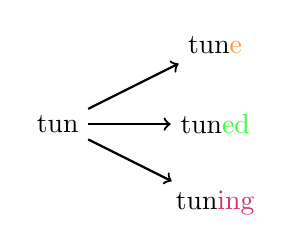
\begin{tikzpicture}
    \node (tun) at (-1,0) {tun};
    \node (tune) at (1, 1) {tun\color{orange!80}{e}};
    \node (tuned) at (1, 0) {tun\color{green!80}{ed}};
    \node (tuning) at (1, -1) {tun\color{purple!80}{ing}};
    \draw[->,thick] (tun) -> (tune);
    \draw[->,thick] (tun) -> (tuned);
    \draw[->,thick] (tun) -> (tuning);
  \end{tikzpicture}
\end{center}

If we were to perform stemming on our entire corpus, the words ``tune'', ``tuned'', and ``tuning'' all get reduced to the stem ``tun''. So, your vocabulary would be significantly reduced in performing this process. You can further reduce the size of the vocabulary without losing valuable information by \emph{lower-casing} every word, e.g. the words ``GREAT'', ``Great'', and ``great'' all get treated as the same word. Perhaps our final preprocessed tweet looks like
\begin{verbatim}
[tun, great, ai, model]
\end{verbatim}

In summary, for our example of sentiment analysis on tweets, we might preprocess as follows:
\begin{enumerate}
\item Eliminate handles and URLs
\item Tokenize the string into words
\item Remove stop words like ``and, is, a, on, etc.''
\item Stemming - or convert every word to its stem. E.g. dancer, dancing,   danced, becomes ``danc''. You can use \href{https://tartarus.org/martin/PorterStemmer/}{Porter Stemmer} to take care of this.
\item Convert all words to lowercase.
\end{enumerate}

As an applied example:
$$
\textrm{I am Happy Because I am learning NLP @deeplearning} \overset{\small \textrm{Preprocessing}}{\longrightarrow} [\texttt{happy, learn, nlp}] \overset{\small \textrm{Feature Extraction}}{\longrightarrow} [1, 4, 2]
$$
where 1 is our bias term, 4 is the sum of positive frequencies, and 2 is the sum of negative frequencies.
In practice, we are given a set of $m$ raw tweets, and so wehave to process them one-by-one to process them into an $m \times 3$ matrix, where each row describes the features for a given tweet.

\begin{equation*}
  \begin{bmatrix}
    1 & X_1^{(1)} & X_2^{(1)} \\
    1 & X_1^{(2)} & X_2^{(2)} \\
    \vdots & \vdots & \vdots \\
    1 & X_1^{(m)} & X_2^{(m)} \\
  \end{bmatrix}
\end{equation*}

The process is simple: (i) build the frequencies dictionary, (ii) initialize the matrix $X$ to match the number of tweets, (iii) go through your sets of tweets and carefully preprocess by deleting stop words, stemming, deleting URLs/handles, and lowercasing, and finally (iv) extract the features by summing up the positive and negative frequencies of each of the tweets.

\begin{python}
freqs = build_freqs(tweets, labels)          # Build frequencies dictionary.
X = np.zeros((m,3))                          # Initialize matrix X.
for i in range(m):                           # For every tweet:
  p_tweet = process_tweet(tweets[i])         #   Process tweet.
  X[i,:] = extract_features(p_tweet, freqs)  #   Extract features.
\end{python}

\subsection{Logistic Regression} Previously, we've learned how to extract features, which we will now use to predict whether a tweet has a positive or negative sentiment. Logistic regression makes use of a \href{https://en.wikipedia.org/wiki/Logistic_function#Mathematical_properties}{sigmoid (or standard logistic) function} which outputs a probability between zero and one. What's the recap from supervised machine learning? Recall figure \ref{fig: supervised_ml}: in the case of logistic regression our prediction function is going to be the standard logistic function:

\[
  h(x^{(i)}, \theta) = \frac{1}{1 + e^{-\theta^T x^{(i)}}}.
\]
where $i$ denotes the observation number. Note that as $\theta^T x^{(i)}$ gets closer and closer to $-\infty$, the denominator of the sigmoid expression blows up and as a result the output values gets closer to zero. Conversely, as the inner product $\theta^T x^{(i)}$ gets closer to $\infty$, the denominator of the sigmoid function approaches unit value and the resulting sigmoid expression evaluates to something near one.
For classification, a threshold is needed, and it is natural to set it at $\frac{1}{2}$. For the logistic function, this threshold occurs when the inner product $\theta^T x^{(i)} = 0$. If the inner product is greater than (or equal to) zero, we classify as positive, else negative.

\subsubsection{Learning Parameters}
\paragraph{How to learn $\theta$?} To train a logistic regression classifier, we need to iterate until we find a set of parameters $\theta$ that minimizes our cost function. Suppose we have a loss that depends only on the parameters $\theta_1, \theta_2$: you might have a cost function that looks like follows, on the left, with the evaluation of the cost function plotted on the right as a function of the number of training iterations:

\begin{minipage}{1.0\textwidth}
  \begin{multicols}{2}
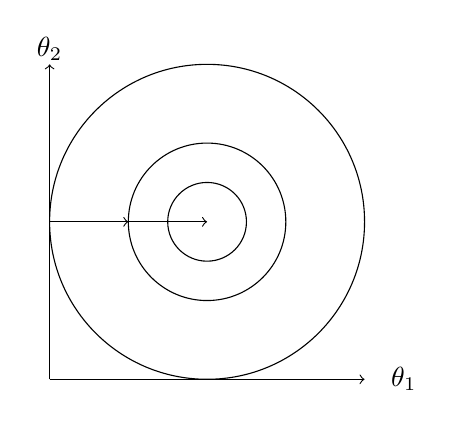
\begin{tikzpicture}[scale=2]
  \draw[->] (-1, -1) to (-1, 1);
  \node at (-1, 1.1) {$\theta_2$};
  \draw[->] (-1, -1) to (1, -1);
  \node at (1.25, -1) {$\theta_1$};
  \draw (0, 0) circle (1cm);   
  \draw (0, 0) circle (.5cm); 
  \draw (0, 0) circle (.25cm); 
  \draw[->] (-1, 0) to (-.5, 0);
  \draw[->] (-.5, 0) to (0, 0);
\end{tikzpicture}
\vfill\null \columnbreak
\begin{tikzpicture}[scale=3]
  \draw[->] (0, 0) to (0, 1.4) node [left] {cost};
  \draw[->] (0, 0) to (2.1, 0) node [right]{\# iterations}; 
  \draw[smooth, domain=0.2:2, color=orange, thick]
    plot (\x,{exp(-\x)}) {};
\end{tikzpicture}
\end{multicols}
\end{minipage}

We might first initialize our parameters $\theta$, then update our parameters in the direction of the \emph{gradient of the cost function}. After a sufficient number of training steps, we will have updated $\theta$ to their optimal values where we are achieving near optimal cost. Let's quickly review this process of gradient descent for logistic regression:

\begin{figure}[h]
\begin{center}
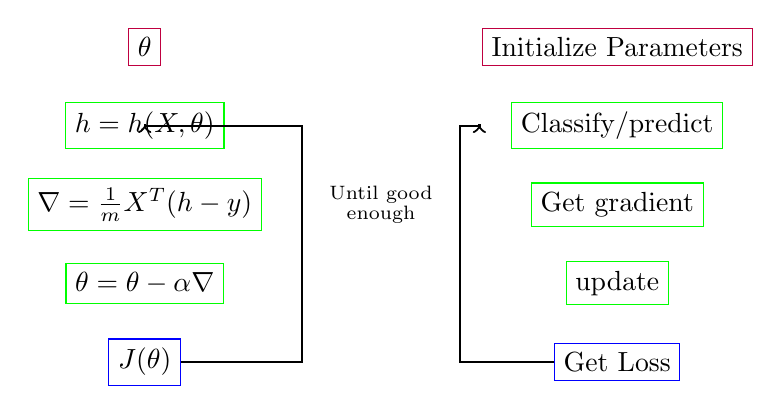
\begin{tikzpicture}
  % Left partition
  \node[draw,rectangle,color=purple] (theta) at (-2, 2) {\color{black}$\theta$};
  \node[draw,rectangle,color=green] (h) at (-2, 1) {\color{black}$h = h(X,\theta)$};
  \node[draw,rectangle,color=green] (gradient) at (-2, 0) {\color{black}$\nabla = \frac{1}{m} X^T (h-y)$};
  \node[draw,rectangle,color=green] (update_eq) at (-2, -1) {\color{black}$\theta = \theta - \alpha \nabla$};
  \node[draw,rectangle,color=blue] (cost) at (-2, -2)   {\color{black}$J(\theta)$};
  \draw[->,thick] (cost) -- ++(2, 0) -- ++(0,3) -| (h);
  % Right partition
  \node[draw,rectangle,color=purple] (init) at (4, 2) {\color{black}Initialize Parameters};
  \node[draw,rectangle,color=green] (classifypredict) at (4, 1) {\color{black}Classify/predict};
  \node[draw,rectangle,color=green] (gradient) at (4, 0) {\color{black}Get gradient};
  \node[draw,rectangle,color=green] (update_eq) at (4, -1) {\color{black}update};
  \node[draw,rectangle,color=blue] (getloss) at (4, -2)   {\color{black}Get Loss};
\draw[->,thick] (getloss) -- ++(-2, 0) -- ++(0,3) -| ++(0.25, 0);

% Middle comment
\node at (1, 0) {$\substack{\textrm{Until good} \\ \textrm{enough}}$};
\end{tikzpicture}
\end{center}
\end{figure}

\subsubsection{Assessing model generalization}
To analyze model fit, we need the following: $(X_{\textrm{val}}, Y_{\textrm{val}}, \theta)$, where we have \emph{validation} data that was set aside during training, and a learned $\theta$ parameter vector. We will compute, for each example in $X_{\textrm{val}}$, the value of $h(\theta, x^{(i)})$ and compare it with our threshold value to make a prediction. In particular, our simple prediction function is given by
\[
  \hat Y_{\textrm{val}} = h(X_{\textrm{val}}, \theta) \geq \frac{1}{2}.
\]

In particular, we will have a vector $h = \begin{bmatrix} h_1 & h_2 & \ldots & h_m \end{bmatrix}$ where e.g. $h_i$ could equal some float in $[0,1]$, which we then convert into a binary label vector by applying our threshold. After building our predictions vector $\hat Y_{\textrm{val}}$, we can compare the predictions with the actual values and evaluate our test-set \emph{accuracy}:

\begin{equation*}
\texttt{Accuracy} = \sum_{i=1}^m \frac{\left(\texttt{pred}^{(i)} == \hat Y_{\textrm{val}}^{(i)}\right)}{m}.
\end{equation*}

This metric gives an estimate of the number of times of logistic regression model will work correctly on unseen data.

\subsubsection{Deriving Gradient Descent for Logistic Regression}
\paragraph{Motivating where cost function comes from} Let's examine the equation for the cost function for logistic regression:

\begin{equation}
  \label{eq: crossentropyloss}
  J(\theta) = -\frac{1}{m} \sum_{i=1}^{m} \left[ y^{(i)} \log h(x^{(i)}, \theta) + (1 - y^{(i)}) \log \left(1 - h(x^{(i)}, \theta)\right)\right].
\end{equation}

The deep learning notes derive this equation in detail in the introduction. Let us briefly recap.
\[
  \Pr(y | x^{(i)}, \theta) = h(x^{(i)}, \theta)y^{(i)}\left(1 - h(x^{(i)}, \theta)\right)^{(1-y^{(i)})}.
\]

We wish to maximize our function $h(\cdot, \theta)$ over the parameter space $\theta$: when $y=0$ we want $(1 - h(x^{(i)}, \theta))$ to be zero, and therefore $h(x^{(i)}, \theta)$ close to one. When $y=1$, we want $h(x^{(i)},\theta) = 1$. To model our entire dataset and not just one observation, we make an assumption of independence to arrive at a joint likelihood:
\[
  L(\theta) = \prod_{i=1}^m h(x^{(i)}, \theta)^{y^{(i)}} \left(1 - h(x^{(i)}, \theta)\right)^{(1 - y^{(i)})}.
\]

Realize that if we ``mess up'' one prediction, we have the potential to ``mess up'' the entire cost function, which is what we want: we want a model that captures the entire dataset, where all datapoints are related. One issue: what happens when $m$ grows? Then $L(\theta) \leadsto 0$, because the expressions
$h(x^{(i)}, \theta)$ and correspondingly $(1 - h(x^{(i)}, \theta)$ are bounded between $(0,1)$.

\paragraph{Optimization}
Using properties of logarithms (that they are monotone and maximizing a function under a monotone transformation doesn't change the optimum, and that they turn multiplication into addition), i.e.
\begin{align*}
  \log(a*b*c) = \log a + \log b + \log c \, \, \, \, \, \textrm{ and } \, \, \, \, \, \log a^b = b \log a.
\end{align*}
We may now rewrite our optimization problem:
\begin{align*}
  \max_{h(x^{(i)}, \theta)} \log L(\theta) &= \log \prod_{i=1}^{m} h(x^{(i)},                                              \theta)^{y^{(i)}} \left(1 - h(x^{(i)}, \theta)\right)^{1 - y^{(i)}} \\
  &= \sum_{i=1}^{m} \log h(x^{(i)}, \theta)^{y^{(i)}} \left(1 - h(x^{(i)},     \theta)\right)^{1 - y^{(i)}} \\
  &= \sum_{i=1}^{m} \log h(x^{(i)}, \theta)^{y^{(i)}}  + \log \left(1 - h(x^{(i)}, \theta)\right)^{1 - y^{(i)}} \\
  &= \sum_{i=1}^{m} y^{(i)} \log h(x^{(i)}, \theta) + (1 - y^{(i)}) \log \left(1 - h(x^{(i)}, \theta)\right)  
\end{align*}

We can then rescale by $\frac{1}{m}$ to get \emph{average} cost. Recall we are maximizing over $h(x^{(i)}, \theta)$ in the equation above, and maximizing an equation is the same as minimizing its negative. Therefore,
\[
  J(\theta) = -\frac{1}{m} \sum_{i=1}^{m} \left[ y^{(i)} \log h(x^{(i)}, \theta) + (1 - y^{(i)}) \log \left(1 - h(x^{(i)}, \theta)\right)\right]. 
\]

A vectorized implementation is given by
\begin{align*}
  h &= g(X\theta) \\
  J(\theta) &= \frac{1}{m} \cdot \left(-y^T \log(h) - \left(1 - y \right)^T \log (1 - h)\right)
\end{align*}

\paragraph{Intuition for loss function of logistic regression}
Now, let's just go over some intuition here. Consider the term on the left-hand side of the parenthesized expression: this is the relevant term in your cost function when your label is 1. The term on the right is relevant when the label is zero. In general, this loss function simply says: the closer the prediction is to the observed label, the smaller the loss incurred. We can plot the cost as a function of our the prediction value for a single training example.

\begin{minipage}{1.0\textwidth}
  \begin{multicols}{2}
    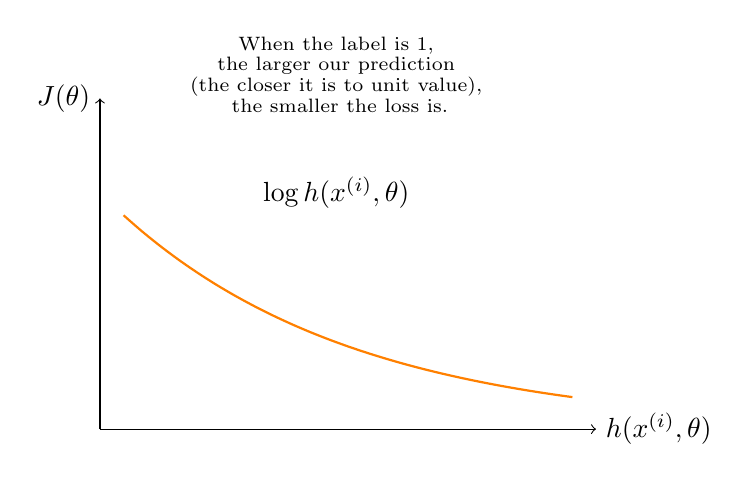
\begin{tikzpicture}[scale=3]
      \draw[->] (0, 0) to (0, 1.4) node [left] {$J(\theta)$};
      \draw[->] (0, 0) to (2.1, 0) node [right]{$h(x^{(i)}, \theta)$}; 
      \draw[smooth, domain=0.1:2, color=orange, thick]
      plot (\x,{exp(-\x)}) {};
      % plot (\x,{-log2(\x/2)}) {};
      \node at (1, 1) {$\log h(x^{(i)}, \theta)$};
      \node at (1, 1.5) {$\substack{\textrm{When the label is 1,} \\ \textrm{the larger our prediction} \\ \textrm{(the closer it is to unit value),} \\ \textrm{ the smaller the loss is.}}$};
    \end{tikzpicture}
    \vfill\null \columnbreak
    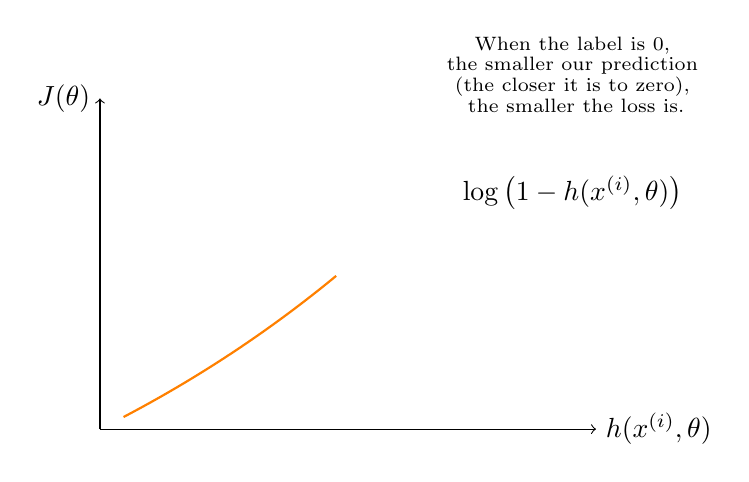
\begin{tikzpicture}[scale=3]
      \draw[->] (0, 0) to (0, 1.4) node [left] {$J(\theta)$};
      \draw[->] (0, 0) to (2.1, 0) node [right]{$h(x^{(i)}, \theta)$}; 
      \draw[smooth, domain=0.1:1, color=orange, thick]
      % plot (\x,{\x^2}) {};
      plot (\x, {exp(\x/2)-1}) {};
      \node at (2, 1) {$\log \left(1 -  h(x^{(i)}, \theta)\right)$};
      \node at (2, 1.5) {$\substack{\textrm{When the label is 0,} \\ \textrm{the smaller our prediction} \\ \textrm{(the closer it is to zero),} \\ \textrm{ the smaller the loss is.}}$};
\end{tikzpicture}
\end{multicols}
\end{minipage}

\newpage
\paragraph{Deriving logistic regression gradient}
The general form of logistic regression is given by

\begin{algorithm}
  \caption{General form of gradient descent}
  \While{not converged, and for all $j$}{
    $\theta_j \gets \theta_j - \alpha \frac{\partial}{\partial \theta_j}     J(\theta)$
  }
\end{algorithm}

We can work out the derivative using partial calculus to fill in the expression further:

\begin{algorithm}
  \caption{Gradient descent for logistic regression}
  \While{not converged, and for all $j$}{
    $\theta_j \gets \theta_j - \frac{\alpha}{m} \sum_{i=1}^m \left(h(x^{(i)}, \theta) - y^{(i)}\right) x_j^{(i)}$
  }
\end{algorithm}

A vectorized implementation is given by
\[
  \theta := \theta - \frac{\alpha}{m} X^T \left(H(X,\theta) - Y\right).
\]

\paragraph{Partial derivative of $J(\theta)$} It'll be helpful to first calculate the derivative of the sigmoid function.
\begin{align*}
  h(x)' &= \left( \frac{1}{1 + e^{-x}} \right)' = \frac{-(1 + e^{-x})'}{(1 + e^{-x})^2} = \frac{-1' - (e^{-x})'}{(1 + e^{-x})^2} = \frac{0 -           (-x)'(e^{-x})}{(1 + e^{-x})^2} = \frac{e^{-x}}{(1 + e^{-x})^2} \\
        &= \left( \frac{1}{1 + e^{-x}} \right) \left( \frac{e^{-x}}{1 + e^{-x}} \right) = h(x) \left( \frac{+1 - 1 + e^{-x}}{1 + e^{-x}} \right) = h(x) \left(\frac{1+e^{-x}}{1+e^{-x}} - \frac{1}{1+e^{-x}}\right) = h(x) (1 - h(x)).
\end{align*}

The above was all for a computation of the derivative of the sigmoid function. But what about the derivative of $h(x^{(i)}, \theta) = \frac{1}{1 + e^{-\theta^T x^{(i)}}}$ with respect to $\theta_j$? Using the chain rule, because of the inner product $\theta^T x^{(i)}$, and applying toward $\theta_j$, we see that the derivative would be
\[
  h(x^{(i)},\theta)\left(1 - h(x^{(i)},\theta)\right) x_j^{(i)}.
\]

Now, we can compute the partial derivative of our loss function with respect to $\theta_j$:

\begin{align*}\frac{\partial}{\partial \theta_j} J(\theta) &= \frac{\partial}{\partial \theta_j} \frac{-1}{m}\sum_{i=1}^m \left [ y^{(i)} log ( h(x^{(i)}, \theta) ) + (1-y^{(i)}) log (1 -  h(x^{(i)}, \theta)) \right ] \\ &= - \frac{1}{m}\sum_{i=1}^m \left [     y^{(i)} \frac{\partial}{\partial \theta_j} log ( h(x^{(i)}, \theta))   + (1-y^{(i)}) \frac{\partial}{\partial                                                                                  \theta_j} log (1 -  h(x^{(i)}, \theta))\right ] \\
                                                           &= - \frac{1}{m}\sum_{i=1}^m \left [     \frac{y^{(i)} \frac{\partial}{\partial \theta_j}  h(x^{(i)}, \theta)}{ h(x^{(i)}, \theta)}   + \frac{(1-y^{(i)})\frac{\partial}{\partial                                                      \theta_j} (1 -  h(x^{(i)}, \theta))}{1 -  h(x^{(i)}, \theta)}\right ] \\
                                                           &= - \frac{1}{m}\sum_{i=1}^m \left [     \frac{y^{(i)} \frac{\partial}{\partial \theta_j}  h(x^{(i)}, \theta)}{ h(x^{(i)}, \theta)}   + \frac{(1-y^{(i)})\frac{\partial}{\partial \theta_j} (1 -  h(x^{(i)}, \theta))}{1                                                              -  h(x^{(i)}, \theta)}\right ] \\
                                                           &= - \frac{1}{m}\sum_{i=1}^m \left [     \frac{y^{(i)}  h(x^{(i)}, \theta) (1 -  h(x^{(i)}, \theta)) \frac{\partial}{\partial \theta_j} \theta^T x^{(i)}}{ h(x^{(i)}, \theta)}   + \frac{- (1-y^{(i)})  h(x^{(i)}, \theta)(1 -  h(x^{(i)}, \theta)) \frac{\partial}{\partial \theta_j} \theta^T x^{(i)}}{1 -  h(x^{(i)},                                                              \theta)}\right ] \\
                                                           &= - \frac{1}{m}\sum_{i=1}^m \left [     \frac{y^{(i)}  h(x^{(i)}, \theta) (1 -  h(x^{(i)}, \theta)) \frac{\partial}{\partial \theta_j} \theta^T x^{(i)}}{ h(x^{(i)}, \theta)}   - \frac{(1-y^{(i)}) h(x^{(i)}, \theta) (1 -  h(x^{(i)}, \theta)) \frac{\partial}{\partial \theta_j} \theta^T x^{(i)}}{1 -  h(x^{(i)},                                                              \theta))}\right ] \\
                                                           &= - \frac{1}{m}\sum_{i=1}^m \left [     y^{(i)} (1 -  h(x^{(i)}, \theta)) x^{(i)}_j                                                              - (1-y^{(i)})  h(x^{(i)}, \theta) x^{(i)}_j\right ] \\
                                                           &= - \frac{1}{m}\sum_{i=1}^m \left [     y^{(i)} (1 -  h(x^{(i)}, \theta)) -                                                              (1-y^{(i)})  h(x^{(i)}, \theta) \right ] x^{(i)}_j \\
                                                           &= - \frac{1}{m}\sum_{i=1}^m \left [     y^{(i)} - y^{(i)}  h(x^{(i)}, \theta) -                                                               h(x^{(i)}, \theta) + y^{(i)}  h(x^{(i)}, \theta) \right ] x^{(i)}_j \\
                                                           &= - \frac{1}{m}\sum_{i=1}^m \left [ y^{(i)} -  h(x^{(i)}, \theta) \right ] x^{(i)}_j    \\
                                                           &= \frac{1}{m}\sum_{i=1}^m \left [  h(x^{(i)},                               \theta) - y^{(i)} \right ] x^{(i)}_j
\end{align*}
The vectorized version is simply given by
\[
  \nabla J(\theta) = \frac{1}{m} \cdot X^T \left( H(X, \theta) - Y \right).
\]

\section{Sentiment Analysis with Naive Bayes}\vspace{.1pt} \hrule height 2pt \smallskip \renewcommand{\arraystretch}{1}% Tighter
\subsection{Probability and Bayes Rule} Imagine you have an extensive corpus of tweets that can be categorized as either positive or negative, but not both.


\begin{minipage}{1.0\textwidth}
\begin{multicols}{2}
  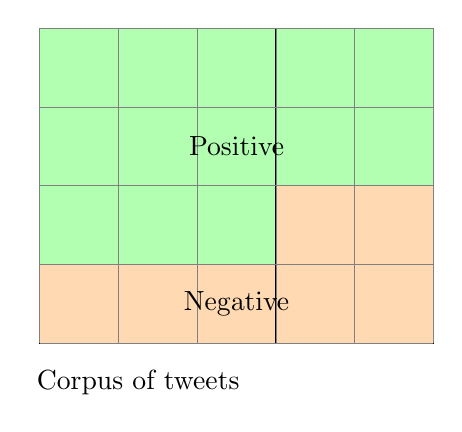
\begin{tikzpicture}
    \draw[fill=green!30] (0, 1) rectangle (3, 4);
    \draw[fill=orange!30] (0, 0) rectangle (3, 1);
    \draw[fill=orange!30] (3, 0) rectangle (5, 2);
    \draw[fill=green!30] (3, 2) rectangle (5, 4);
    \draw[step=1cm, gray, very thin] (0, 0) grid (5, 4);
    \node (neg) at (2.5, 0.5) {Negative};
    \node (pos) at (2.5, 2.5) {Positive};
    \node at (1.25, -0.5) {Corpus of tweets};
  \end{tikzpicture}
  \vfill\null \columnbreak
  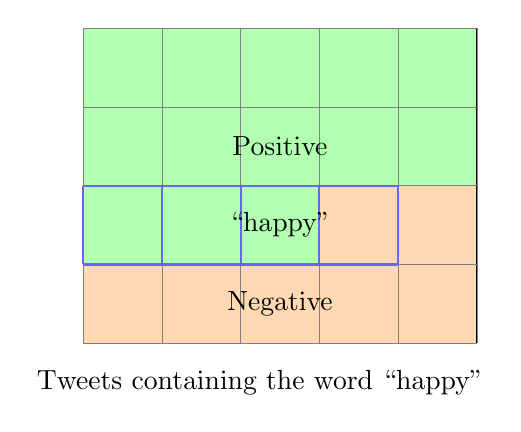
\begin{tikzpicture}
    \draw[fill=green!30] (0, 1) rectangle (3, 4);
    \draw[fill=orange!30] (0, 0) rectangle (3, 1);
    \draw[fill=orange!30] (3, 0) rectangle (5, 2);
    \draw[fill=green!30] (3, 2) rectangle (5, 4);
    \draw[step=1cm, gray, very thin] (0, 0) grid (5, 4);
    \node (neg) at (2.5, 0.5) {Negative};
    \node (pos) at (2.5, 2.5) {Positive};
    \draw[step=1cm, blue!60, thick] (0, 1) grid (4, 2);
    \node (happy) at (2.5, 1.5) {``happy''};
    \node at (2.25, -0.5) {Tweets containing the word ``happy''};
  \end{tikzpicture}
\end{multicols}
\end{minipage}

Within this corpus, observe that the word ``happy'' is sometimes associated with a positive sentiment, but also sometimes with a negative sentiment! How can this happen? Let's explore the situation using probabilities.

\paragraph{Intro probability} Suppose we define an event $A$ as a positive tweet. Then, $\Pr(A) = \Pr(\textrm{Positive}) = \frac{N_{\textrm{pos}}}{N}$, i.e. the ratio between the number of positive-sentiment tweets relative to the total number of tweets observed in our data. In our example above, it comes out $\frac{13}{20}$.\footnote{Of course, because tweets can only be positive or negative but not both, the probability of a negative tweet is simply the complement, i.e. $\Pr(\textrm{Negative}) = 1 - \Pr(\textrm{Positive})$ which in our example happens to be $\frac{7}{20}$.} Let's define an event $B$ as a tweet containing the word ``happy''. In our examples above, this happens to be four, i.e. $\Pr(B) = \Pr(\textrm{``happy''}) = \frac{N_{\textrm{happy}}}{N}$ is $\frac{4}{20}$. Building on this, $\Pr(A \land B) = \Pr(A,B)$ which happens to be $\frac{3}{20}$ in our pictorial example above.

\paragraph{Deriving Bayes rule} What if instead of the entire corpus, we only consider tweets that contain the word ``happy''? $\Pr(A|B) = \Pr(\textrm{Positive} | \textrm{``happy''}) = \frac{3}{4}$ in our example. But we can also do the same thing for positive tweets, i.e.
\[
  \Pr(B|A) = \Pr(\textrm{``happy''} | \textrm{Positive}) = \frac{3}{13}.
\]

There are two equivalent ways of thinking about conditional probabilities:
\begin{figure}[h]
  \begin{center}
    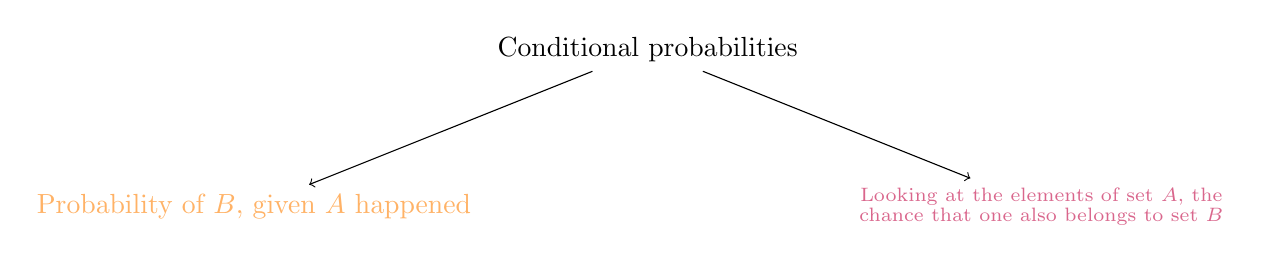
\begin{tikzpicture}
      \node (cp) at (0, 0) {Conditional probabilities};
      \node (l) at (-5, -2) {\color{orange!60} Probability of $B$, given $A$         happened};
      \node (r) at (5, -2) {\color{purple!60} $\substack{\textrm{Looking at the elements of set } A, \textrm{ the} \\ \textrm{chance that one also belongs to set } B}$};
\draw[->] (cp) -- (l);
\draw[->] (cp) -- (r);
    \end{tikzpicture}
  \end{center}
\end{figure}

So, in our context:
\begin{equation}
  \label{eq: bayes1}
  \Pr(\textrm{Positive} | \textrm{``happy''}) = \frac{\Pr(\textrm{Positive} \land \textrm{``happy''})}{\Pr(\textrm{``happy''})}.
\end{equation}

And by symmetry:
\begin{equation}
  \label{eq: bayes2}
  \Pr(\textrm{``happy''} | \textrm{Positive}) = \frac{\Pr(\textrm{``happy''} \land \textrm{Positive})}{\Pr(\textrm{Positive})}.
\end{equation}

Realize that the intersection operation between two events is symmetric, i.e. that the numerator in equations \ref{eq: bayes1} and \ref{eq: bayes2} are identical. Therefore,
\begin{equation}
  \label{eq:bayesrulederivation}
  \Pr(\textrm{Positive} | \textrm{``happy''}) = \Pr(\textrm{``happy''} | \textrm{Positive}) \times \frac{\Pr(\textrm{Positive})}{\Pr(\textrm{``happy''})}.
\end{equation}
This is an expression of Bayes rule in the context of the sentiment analysis problem. More generally: Bayes rule specifies that $\Pr(X|Y) = \Pr(Y|X) \times  \frac{\Pr(X)}{\Pr(Y)}$.

\subsection{Naive Bayes}
\label{sec: naivebayes}
Naive Bayes is often a ``very good, quick, and dirty baseline'' for many text classification tasks; it's an example of supervised machine learning and as such shares many similarities with logistic regression. It's called Naive because it makes the assumption that the features you're using for classification are all independent, which in reality is \emph{rarely} the case. As per usual, we start with two corpora: one for the positive tweets and one for the negative tweets:

\begin{minipage}{1.0\textwidth}
  \begin{multicols}{2}
    \begin{center}
  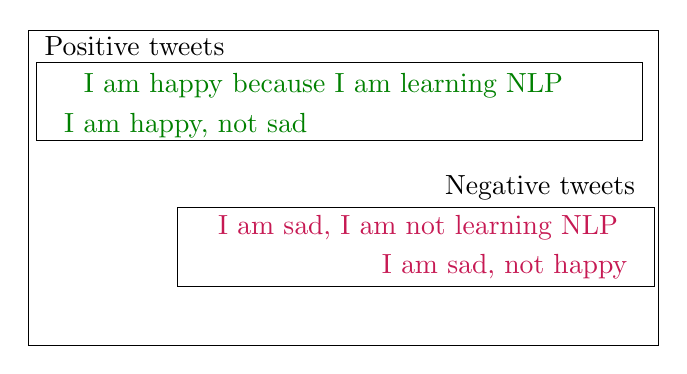
\begin{tikzpicture}
    \draw (0, 2) rectangle (8, -2);
    \node at (1.35, 1.8) {Positive tweets};
    \node at (3.75, 1.3) {\color{green!50!black}I am happy because I am learning NLP};
    \node at (2.00, 0.8) {\color{green!50!black}I am happy, not sad};
    \draw (0.1, 0.6) rectangle (7.8, 1.6);
    \node at (6.5, 0) {Negative tweets};
    \node at (4.95, -0.5) {\color{purple!90} I am sad, I am not learning NLP};
    \node at (6.05, -1) {\color{purple!90} I am sad, not happy};
    \draw (1.9, -1.25) rectangle (7.95, -0.25);
  \end{tikzpicture}
\end{center}
\vfill\null \columnbreak
\begin{tabular}{c c c}
  \hline
  word & {\color{green!50!black} Pos} & {\color{purple!90} Neg} \\
  \hline
  I & 3 & 3 \\
  am & 3 & 3 \\
  happy & 2 & 1 \\
  because & 1 & 0 \\
  learning & 1 & 1 \\
  NLP & 1 & 1 \\
  sad & 1 & 2 \\
  not & 1 & 2 \\
  \hline
  $N_{\textrm{class}}$ & 13 & 13
\end{tabular}
\end{multicols}
\end{minipage}

The above word frequencies table is the backbone input to our naive bayes algorithm: it allows us to compute conditional probabilities. E.g. $\Pr(\textrm{I} | \textrm{Pos}) = \frac{3}{13}$. We can do this for each word in our vocabulary, i.e. compute the conditional probability of it appearing in each class. Notice that if you sum over the probabilities for a particular class, you get 1.

\begin{center}
\begin{tabular}{c c c}
  \hline
  word & {\color{green!50!black} Pos} & {\color{purple!90} Neg} \\
  \hline
  I & $\frac{3}{13}$ & $\frac{3}{13}$ \\
  am & $\frac{3}{13}$ & $\frac{3}{13}$ \\
  {\color{green!50!black} happy} & $\frac{2}{13}$ & $\frac{1}{13}$ \\
  because & $\frac{1}{13}$ & 0 \\
  learning & $\frac{1}{13}$ & $\frac{1}{13}$ \\
  NLP & $\frac{1}{13}$ & $\frac{1}{13}$ \\
  {\color{purple!90}sad} & $\frac{1}{13}$ & $\frac{2}{13}$ \\
  {\color{purple!90}not} & $\frac{1}{13}$ & $\frac{2}{13}$ \\
  \hline
  Sum & 1 & 1
\end{tabular}
\end{center}

Let's inspect some of the entries: notice that for a few words in the vocabulary, their conditional probabilities of appearing in either class are (nearly) identical: words that are equally probable don't add anything to the sentiment. On the other hand, words like {\color{green!50!black} happy}, or {\color{purple!90} sad, not} are ``power'' words which tend to express one sentiment or another. These words carry a lot of weight in determining your tweet sentiments. As a separate note, examine the word \texttt{because}: it only appears in the positive corpus, and so its conditional probability for the negative class is zero: when this happens we have no way of comparing between the two corpora which will become a problem for subsequent calculations. We'll see how we can ``smooth'' our probability function.

Suppose we get a new tweet, ``I am happy today; I am learning.'' and we want to classify its sentiment. We use the following expression:
\[
  \prod_{i=1}^{m} \frac{\Pr(w_i | \textrm{pos})}{\Pr(w_i|\textrm{neg})}
\]

So, for our tweet example, we have (word by word, and skipping ``today'' because it doesn't appear in our vocabulary):
\[
  \frac{\frac{3}{13}}{\frac{3}{13}} \times \frac{\frac{3}{13}}{\frac{3}{13}} \times \frac{\frac{2}{13}}{\frac{1}{13}} \times \frac{\frac{3}{13}}{\frac{3}{13}} \times \frac{\frac{3}{13}}{\frac{3}{13}} \times \frac{\frac{1}{13}}{\frac{1}{13}} = \frac{2}{13} {\color{green!50!black} > 1}.
\]

Because the ratio is greater than unit value, we conclude that overall the sentiment of the tweet is positive.

\paragraph{Laplacian smoothing} This is a technique we use to avoid probabilities being identically zero. Typically, the expression used to calculate the conditional probability of a word, given the class, is
\[
  \Pr(w_i | \textrm{class}) = \frac{\texttt{freq}(w_i, \textrm{class})}{N_{\textrm{class}}} \hspace{35pt} \textrm{class} \, \in \, \{\textrm{Positive}, \textrm{Negative}\}
\]
where $N_{\textrm{class}} = \textrm{ frequency of all words in class}$. Laplacian smoothing does the following; supposing $|V|$ is the number of unique words in the vocabulary
\begin{equation}
  \label{eq: laplaciansmoothing}
  \Pr(w_i | \textrm{class}) = \frac{\texttt{freq}(w_i, \textrm{class}) + 1}{N_{\textrm{class}} + |V|}.  
\end{equation}

By adding a one to our numerator, we ensure the expression is non-zero. However, this is not correctly normalized by $N_{\textrm{class}}$, and so we add a new term to the denominator $|V|$; this ensures the probabilities all sum to one. E.g. in our example table in section \ref{sec: naivebayes} describing positive and negative word frequencies in our corpora of tweets, we can use this to compute
\[
  \Pr(\textrm{I} | \textrm{Pos}) = \frac{3+1}{13+8}.
\]
We can apply Laplacian smoothing to every entry in our table and end up with a new table of conditional probabilities where the column-sums are unit valued.
Notice that if we apply this technique to the word ``because'' in our example, and specificially for the negative class, that $\Pr(\textrm{because} | \textrm{Negative}) = \frac{0 + 1}{13 + 8} > 0$ which solved our original problem of getting a divide by zero in the formula for Naive Bayes $\prod_{i=1}^m \frac{\Pr(w_i | \textrm{Pos})}{\Pr(w_i | \textrm{Neg})}$.

\paragraph{Log likelihoods} Words can have many shades of emotional meaning, but for the purpose of sentiment classification they can be simplified into three categories: neutral, positive, and negative. A word can be taxonomized according to its conditional probabilities. We simply calculate for each word
\[
  \textrm{ratio}(w_i) = \frac{\Pr(w_i | \textrm{{\color{green!50!black}\textrm{Pos}}})}{\Pr(w_i | {\color{purple!90} \textrm{Neg}})} \approx \frac{\texttt{freq}(w_i, {\color{green!50!black} 1}) + 1}{\texttt{freq}(w_i, {\color{purple!90} 0}) + 1}.
\]

If this ratio is identically unit valued, the word is neutral. Words that are more positive tend to have higher ratios (larger than one), and words that are more negative tend to have lower ratios (less than one). Observe that the ratio can lie in $[0, \infty)$.

It turns out that in our previous formulation of Naive Bayes, we assumed balanced class sizes. The correct formula for the likelihood includes the prior ratio, which becomes important for unbalanced datasets (where e.g. the number of positive and negative tweets is not equal):
\begin{equation}
  \label{eq: completenaivebayeswithprior}
  \frac{\Pr(\textrm{Pos})}{\Pr(\textrm{Neg})} \prod_{i=1}^{m} \frac{\Pr(w_i | \textrm{pos})}{\Pr(w_i|\textrm{neg})}  
\end{equation}

Recognize that this computation involves the product of many probabilities that lie in $(0,1]$, and we run the risk of numerical underfluw if the number returned ``is so small it can't be stored on your device''. There is a nice mathematical trick that avoids this pitfall, and that's to use properties of logarithms: $\log(a \times b) = \log (a) + \log (b)$.
\[
\log  \frac{\Pr(\textrm{Pos})}{\Pr(\textrm{Neg})} \prod_{i=1}^{m} \frac{\Pr(w_i | \textrm{pos})}{\Pr(w_i|\textrm{neg})}  \leadsto \underbrace{\log \frac{\Pr(\textrm{Pos})}{\Pr(\textrm{Neg})}}_{\textrm{log prior}} + \underbrace{\sum_{i=1}^{m} \log \frac{\Pr(w_i | \textrm{Pos})}{\Pr(w_i | \textrm{Neg})}}_{\textrm{log likelihood}}.
\]
Let $\lambda(w) = \log \frac{\Pr(w | \textrm{Pos})}{\Pr(w | \textrm{Neg})}$; we calculate this for each word in our vocabulary. Realize that neutral words (i.e. ones where $\Pr(w | \textrm{Pos}) = \Pr(w | \textrm{Neg})$) have $\lambda(w) = \log(1) = 0$. A positive sentiment is indicated by $\lambda(w) > 0$, and correspondingly $\lambda < 0$ indicates a negative sentiment. By using logarithms, we can reduce the risk of numerical underflow.
Realize that our log-likelihood term can be expressed as $\sum_{i=1}^{m} \log \frac{\Pr(w_i | \textrm{Pos})}{\Pr(w_i | \textrm{Neg})} = \sum_{i=1}^m \lambda(w_i) \in (-\infty, \infty)$; we emphasize that our decision boundary is zero with our log-likelihood formula.

\paragraph{Training Naive Bayes} In the context of Naive Bayes, ``train'' means something different than in logistic regression or deep learning: there's no gradient descent; we're just counting word frequencies in a corpus. There are five steps for training a Naive Bayes model:

\begin{enumerate}
\item Collect and annotate corpus (e.g. with positive and negative tweets)
\item Preprocessing (e.g. $\texttt{process\_tweet}(\textrm{tweet}) \leadsto [w_1, w_2, \ldots, ]$)
    \begin{itemize}
    \item Lowercase
    \item Remove punctuation, urls, names, etc.
    \item Remove stop words
    \item Stemming
    \item Tokenize sentences
  \end{itemize}
\item Compute word counts, i.e. $\texttt{freq}(w, \textrm{class})$ and   $N_{\textrm{class}}$.
\item Apply Laplacian smoothing to compute $\Pr(w | \textrm{class}) = \frac{\texttt{freq}(w, \textrm{class}) + 1}{N_{\textrm{class}} +   |V_{\textrm{class}}|}$.
\item Calculate $\lambda(w) = \log \frac{\Pr(w | \textrm{Pos})}{\Pr(w |     \textrm{Neg})}$.
\item Get the log-prior, which involves first counting $D_{\textrm{Pos}} = $ number of positive tweets and $D_{\textrm{Neg}} = $ number of negative tweets, whereby $\log \textrm{ prior } = \log \frac{D_{\textrm{Pos}}}{D_{\textrm{Neg}}}$.\footnote{If the dataset is balanced, the log-prior is zero since $D_{\textrm{Pos}} = D_{\textrm{Neg}}$ and $\log(1) = 0$.}
\end{enumerate}

\paragraph{Testing Naive Bayes} Once you've trained your model, you test it by taking the conditional probabilities derived and using them to predict the sentiments of new unseen tweets. We can evaluate model performance using test set accuracy. In particular, suppose we are given a tweet ``I passed the NLP interview!'', and then after preprocessing we end up with $[\textrm{I, pass, the, NLP, interview}]$. We then look up our $\lambda(w)$'s that were calculated when we ``trained'' our model and compute the score, i.e. the log-prior plus log-likelihood for the unseen test case and compare it to our threshold (of zero). The values of the words that aren't in our vocabulary are treated as neutral (i.e. zeros) and do not contribute to the final score (likelihood) of the unseen word: $\texttt{pred} = \mathbbm 1_{\texttt{score} > 0}$. If we are given a bunch of unseen words, i.e. data set aside during training ($X_{\textrm{val}}, Y_{\textrm{val}}$), we (i) compute $\texttt{score} = \texttt{predict}(X_{\textrm{val}}, \lambda, \texttt{log-prior})$ and then (ii) predict $\texttt{pred} = \mathbbm 1_{\texttt{score} > 0}$, and then (iii) compute test accuracy given by $\frac{1}{m} \sum_{i=1}^m \left(\texttt{pred}_i   == Y_{\textrm{val}_i}\right)$.

\paragraph{Applications of Naive Bayes} There's more we can do than just sentiment analysis. For example, we could do author identification: if you had two large corpora each written by different authors, you could train the model to recognize whether a document was written by one author or the other. Or, if you had some works by Shakespeare and some works by Hemmingway, you could calculate the $\lambda$ for each word to predict how likely a new word is to be used by Shakespeare or alternatively Hemmingway. Another common use is spam filtering: $\frac{\Pr(\textrm{spam} | \textrm{email})}{\Pr(\textrm{non-spam}|\textrm{email})}$. One of the earliest applications of Naive Bayes was to filter between relevant and irrelevant documents in a database. I.e. given a set of keywords in a query, in this case, you can calculate the likelihood of the documents given the query:
\[
  \Pr(\textrm{document}_k | \textrm{query}) \propto \prod_{i=0}^{|\textrm{query}|} \Pr(\textrm{query}_i | \textrm{document}_k).
\]
Then, we have a decision rule that suggests retrieval if $\Pr(\textrm{document}_k | \textrm{query}) > \textrm{threshold}$, and then \emph{sort} the documents based on their likelihoods; perhaps we choose to keep the first $m$ results or ones with a likelihood above a certain threshold. Lastly, we can also use Naive Bayes for word disambiguation, i.e. breaking words down for contextual clarity. Consider that you have two possible interpretations of a given word within a text: let's say you don't know if the word ``bank'' in a text is referring to the bank of a river or a financial institution. To disambiguate your word, calculate the score of the document: $\frac{\Pr(\textrm{river} | \textrm{text})}{\Pr(\textrm{money} |   \textrm{text})}$.

\subsubsection{Assumptions of Naive Bayes} Naive Bayes is a very simple model: it doesn't involve setting any parameters. The method is called ``naive'' because of the assumptions it makes about the data. The first assumption is independence between predictors within each class, and the second has to do class (im)-balance with your validation sets. Let's explore each in detail and how they can affect our results.

\paragraph{Independence} To illustrate what independence between features looks like, lets consider the following example:
\begin{verbatim}
It is sunny and hot in the Sahara Desert.
\end{verbatim}
Naive Bayes assumes the words in a piece of text are independent of one another, but as you can see this is not always the case: the words ``sunny'' and ``hot'' often appear together as they do in this example. When taken together, they might also be related to the thing they're describing like a beach or a desert; so the words in a sentence aren't really independent of one another. But, Naive Bayes assumes that they are. The implication is that we could end up under \emph{or} over estimating the conditional probabilities of individual words. E.g. if your task was to complete the sentence: ``It's always cold and snowy in \{blank\}'', then Naive Bayes might assign equal probability to the words spring, summer, fall, and winter even though from the context winter is the most likely candidate.\footnote{More sophisticated methods can deal with this issue.}

\paragraph{Distribution of training data} A good data set will contain the same proportion of (e.g. positive and negative) classes as a random sample would. However, most available annotated corpora are artificially balanced. E.g. in a real tweet stream a positive tweet is more likely to be sent than a negative tweet. Part of this has to do with platform decisions to perhaps ban content that is inappropriate or contains offensive vocabulary. Assuming that reality behaves as your training corpus could result in a very optimistic \emph{or} pessimistic model.

\subsubsection{Error Analysis} No matter what NLP method you use, you'll one day find yourself faced with an error, e.g. a missclassified sentence. How can we analyze such errors? Let's consider some possible errors in the model prediction that can be caused by:
\begin{itemize}
\item Removing punctuation and stop words -- semantic meaning can be lost in the preprocessing step.
\item Word order -- can affect the meaning of a sentence.
\item Adversarial attacks -- language quirks can confuse Naive Bayes classifiers.
\end{itemize}

\paragraph{Removing punctuation}
Let's consider an example tweet: ``My beloved grandmother :(''. The sad face punctuation in this case is \emph{very} important to the sentiment of the tweet because it tells you what's happening; but, if we remove punctuation then the processed tweet will leave behind a different (positive) sentiment. After processing, we may end up with $[\textrm{belov, grandmoth}]$ which appear positive in nature.

\paragraph{Removing (stop) words}
It's not just about punctuation either, consider as an example ``this is not good, because your attitude is not even close to being nice''. If we remove stop words, we're left with $[\textrm{good, attitude, close, nice}]$. From this set of words, any classifier would infer that the sentiment is positive. There are techniques we will learn about later to handle ``nots'' and word-order. For now, the takeaway is to look at the processed data to make sure your model can get an accurate read.

\paragraph{Word order}
The input pipeline isn't the only source of trouble. E.g. consider the following two tweets:

\begin{verbatim}
I am happy because I did not go.
I am not happy because I did go.
\end{verbatim}

The first is purely positive, the latter is negative. In this case, the ``not'' is important to the sentiment but gets missed by the Naive Bayes classifier: word order can be as important as spelling.

\paragraph{Adversarial attacks}
Lastly, let's discuss adversarial attacks which essentially describe a language phenomenon like sarcasm, irony, and euphemism. Humans pick these up quickly but machines are terrible at it. The tweet, ``This is a ridiculously powerful movie. The plot was gripping and I cried right through until the ending'' contains a somewhat positive movie review, but pre-processing might suggest otherwise. I.e. if we pre-process, you'll get a list of mostly negative words, but these words were in fact used to describe a movie that the author enjoyed. Applying Naive Bayes to this list of words would yield a negative score, unfortunately.

\section{Vector Space Models}\vspace{.1pt} \hrule height 2pt \smallskip \renewcommand{\arraystretch}{1}% Tighter
\subsection{Motivating Vector Space Models}
Let's talk about vector spaces, and what types of information vectors can encode. We'll talk about vector space models, their advantages, and some applications.

Suppose you have two questions:
\begin{verbatim}
Where are you heading?
Where are you from?
\end{verbatim}

The sentences are identical but for the last word. However, the meaning is entirely different. On the other hand, the two questions:
\begin{verbatim}
What is your age?
How old are you?
\end{verbatim}
contain no overlapping words but have identical meaning. Vector space models can identify similarity even when sentences don't share common words; they can also be used for answering paraphrasing, and summarization. One advantage of vector space models is they allow us to capture dependencies between words. E.g.
\begin{verbatim}
You eat cereal from a bowl.
You buy something and someone else sells it.
\end{verbatim}
In the first sentence, the words \emph{cereal} and \emph{bowl} are related (we're eating one thing out of the other). In the second sentence, the latter half of it depends on the first half. Vector space models can capture this and many other types of relationships among different sets of words. When using a vector space models, the way that representations are made are by identifying the \emph{context} around each word in the text, and this captures the relative meaning. ``You shall know a word by the company it keeps'' (John Firth).

\subsection{Word by Word and Word by Doc}
Let's discuss how to construct vectors based off of a co-occurrence matrix. Depending on the task you're trying to solve, you can have several possible designs.

\paragraph{Word by word} To get a vector space model using a word by word design, you'll make a co-occurrence matrix and extract vector representations for the words in your corpus. We'll also discuss how to find relationships between words and vetors, also known as their similarity. We define the \textbf{co-occurrence} of two different words as the number of times they occur together within a certain distance $k$. E.g. suppose our corpus has the following two sentences:
\begin{verbatim}
I like simple data.
I prefer simple raw data.
\end{verbatim}
Then, the row of the co-occurrence matrix corresponding to the word \texttt{data} with a value $k = 2$ would be populated with the following values:

  \begin{table}[h]
    \begin{center}
      \begin{tabular}{l c c c c}
        & simple & raw & like & I \\
        \hline
        data & 2 & 1 & 1 & 0 \\
        \hline
      \end{tabular}
        \caption{The word ``data'' appears within distance one of the word ``simple'' in the first sentence, and within distance two of the word simple in the second example. Both of these are within our tolerance of $k=2$, so the word by word co-occurrence entry for ``data'' and ``simple'' in this example is the value 2. We can proceed to compare the word ``data'' with other words appearing in our vocabulary, populating a representation that is based on word by word co-occurrence counts within a certain window size.}
  \end{center}
\end{table}

With a word by word design, you get a representation with $|V|$ entries, where $V$ is our vocabulary.

\paragraph{Word by document} With a word by document design, you'll count the number of times that words from your vocabulary appear in documents that belong to specific categories.

\begin{center}
  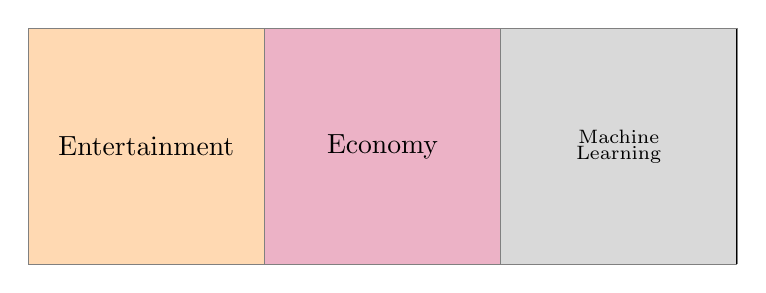
\begin{tikzpicture}[scale=3]
    \draw[fill=orange!30] (0, 0) rectangle (1, 1);
    \draw[fill=purple!30] (1, 0) rectangle (2, 1);
    \draw[fill=gray!30] (2, 0) rectangle (3, 1);
    \draw[step=1cm, gray, very thin] (0, 0) grid (3, 1);
    \node at (0.5, 0.5) {Entertainment};
    \node at (1.5, 0.5) {Economy};
    \node at (2.5, 0.5) {$\substack{\textrm{Machine}\\ \textrm{Learning}}$};
  \end{tikzpicture}
\end{center}

Here, we'd count the number of times that our words appear in the document that belong to each of the three categories. In this example, suppose that the word data appears 500 times in documents from your corpus related to entertainment, 6,620 times in economy documents, and 9,320 in documents related to machine learning. The word film might appear in each document's category 7,000, 4,000, and 1,000 times respectively.

  \begin{table}[h]
    \begin{center}
      \begin{tabular}{l c c c}
        & Entertainment & Economy & $\substack{\textrm{Machine}\\ \textrm{Learning}}$ \\
        \hline
        data & 500 & 6620 & 9320 \\
        film & 7000 & 4000 & 1000 \\
        \hline
      \end{tabular}
    \end{center}
  \end{table}

Once you've constructed representations for multiple sets of documents or words, you'll get your vector space. For example, we could take a representation for the \emph{words} ``data'' and ``film'' by looking at the rows of the table (or matrix). However, we can also get a representation for each \emph{category} of document type by looking at the columns! In our toy example, the vector space will have two dimensions: the number of times that the words ``data'' and ``film'' appear on the type of document.

\begin{figure}[h]
\begin{center}
  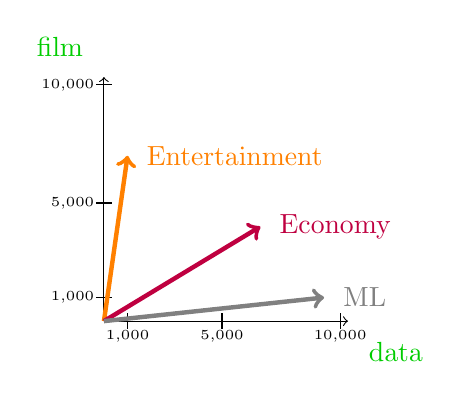
\begin{tikzpicture}
    \draw[->] (0, 0) -- (3.1, 0) node[below right=2mm,color=green!80!black] {data};
    \draw[->] (0, 0) -- (0, 3.1) node[above left=2mm,color=green!80!black] {film};
    % x-axis ticks
    \draw[-] (1.5, -0.1) -- (1.5, 0.1) node[below=1mm] {\tiny 5,000};
    \draw[-] (0.3, -0.1) -- (0.3, 0.1) node[below=1mm] {\tiny 1,000};
    \draw[-] (3.0, -0.1) -- (3.0, 0.1) node[below=1mm] {\tiny 10,000};
    % y-axis ticks
    \draw[-] (-0.1, 1.5) -- (0.1, 1.5) node[left=1mm] {\tiny 5,000};
    \draw[-] (-0.1, 0.3) -- (0.1, 0.3) node[left=1mm] {\tiny 1,000};
    \draw[-] (-0.1, 3.0) -- (0.1, 3.0) node[left=1mm] {\tiny 10,000};
    \draw[->,ultra thick, orange] (0, 0) -- (0.3, 2.1) node[right=1mm] {\color{orange} Entertainment};
    \draw[->,ultra thick, purple] (0, 0) -- (1.986, 1.2) node[right=1mm] {\color{purple} Economy};
    \draw[->,ultra thick, gray] (0, 0) -- (2.796, 0.3) node[right=1mm] {\color{gray} ML};
\end{tikzpicture}
\end{center}
\caption{In this vector representation, the document categories Economy and Machine Learning are more similar to each other than they are to entertainment. Measures of similarity include angle (cosine similarity) and distance (Euclidean, for example).}
\end{figure}

\subsection{Distance and Similarity Metrics}
\paragraph{Euclidean distance}
Euclidean distance is a similarity metric: it identifies how far apart two points (or vectors) are from each other. 

\begin{figure}[h]
\begin{center}
  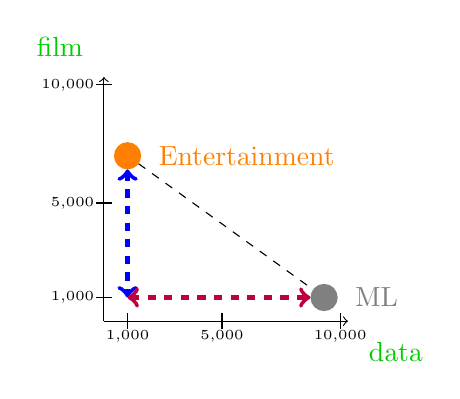
\begin{tikzpicture}
    \draw[->] (0, 0) -- (3.1, 0) node[below right=2mm,color=green!80!black] {data};
    \draw[->] (0, 0) -- (0, 3.1) node[above left=2mm,color=green!80!black] {film};
    % x-axis ticks
    \draw[-] (1.5, -0.1) -- (1.5, 0.1) node[below=1mm] {\tiny 5,000};
    \draw[-] (0.3, -0.1) -- (0.3, 0.1) node[below=1mm] {\tiny 1,000};
    \draw[-] (3.0, -0.1) -- (3.0, 0.1) node[below=1mm] {\tiny 10,000};
    % y-axis ticks
    \draw[-] (-0.1, 1.5) -- (0.1, 1.5) node[left=1mm] {\tiny 5,000};
    \draw[-] (-0.1, 0.3) -- (0.1, 0.3) node[left=1mm] {\tiny 1,000};
    \draw[-] (-0.1, 3.0) -- (0.1, 3.0) node[left=1mm] {\tiny 10,000};
    \node[draw,circle,fill,orange] (e) at (0.3, 2.1) {};
    \node[draw,circle,fill,gray] (ml) at (2.796, 0.3) {};
    \draw[-,dashed] (e) -- (ml);
    \node[right=1mm of e] {\color{orange}Entertainment};
    \node[right=1mm of ml] {\color{gray}ML};
    \draw[<->,dashed,blue, ultra thick] (e) -- (0.3, 0.3);
    \draw[<->,dashed,purple,ultra thick] (0.3,0.3) -- (ml);
\end{tikzpicture}
\end{center}
\caption{Here we visualize the distance between two points, i.e. the length of the line segment connecting them. In two dimensions, this is given by $d(B,A) = \sqrt{({\color{purple} B_1 - A_1})^2 + ({\color{blue}B_2 - A_2})^2}$; the first term is the horizontal distance squared, and the second term is the vertical distance squared.}
\end{figure}

\begin{table}[h]
  \begin{center}
  \begin{tabular}{c | c c c}
    & data & boba & ice-cream \\
    \hline
    AI & 6 & 0 & 1 \\
    drinks & 0 & 4 & 6 \\
    food & 0 & 6 & 8 \\
    \hline
  \end{tabular}
\end{center}
\caption{\small Suppose boba is word $\vec w$ and ice-cream word $\vec v$, and  we wish to calculate the Euclidean distance between these two word-vectors. This is given by $d(\vec v,\vec w) = \sqrt{(1-0)^2 + (6-4)^2 + (8-6)^2} = \sqrt{1 + 4 + 4} = \sqrt{9} = 3$.}
\end{table}

In higher dimensions, i.e. an $n$ dimensional vector, the process is similar.
\[
  d(\vec v,\vec w) = \sqrt{\sum_{i=1}^{n} \left(v_i - w_i\right)^2} = \|\vec v - \vec w\|_2.
\]

\paragraph{Cosine similarity} Another type of similarity function is cosine similarity. Euclidean distance can be problematic: in particular it can be biased by the size difference between the representations; to see why, consider the following example.

\begin{figure}[h]
\begin{center}
  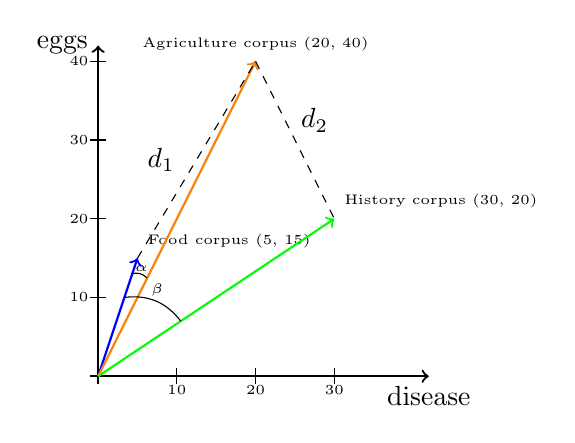
\begin{tikzpicture}
    \draw[->, thick] (-0.1, 0) -- (4.2, 0) node[below] {disease};
    \draw[->, thick] (0, -0.1) -- (0, 4.2) node[left] {eggs};
    % x-axis ticks
    \draw[-] (1, -0.1) -- (1, 0.1) node[below=1mm] {\tiny 10};
    \draw[-] (2, -0.1) -- (2, 0.1) node[below=1mm] {\tiny 20};
    \draw[-] (3, -0.1) -- (3, 0.1) node[below=1mm] {\tiny 30};
    % y-axis ticks
    \draw[-] (-0.1, 1) -- (0.1, 1) node[left=1mm] {\tiny 10};
    \draw[-] (-0.1, 2) -- (0.1, 2) node[left=1mm] {\tiny 20};
    \draw[-] (-0.1, 3) -- (0.1, 3) node[left=1mm] {\tiny 30};
    \draw[-] (-0.1, 4) -- (0.1, 4) node[left=1mm] {\tiny 40};
    \draw[->, thick, blue] (0, 0) -- (0.5, 1.5) node[above right] (fc) {\color{black} \tiny Food corpus (5, 15)};
    \draw[->, thick, orange] (0, 0) -- (2, 4) node[above] (ac) {\color{black} \tiny Agriculture corpus (20, 40)};
    \draw[->, thick, green] (0, 0) -- (3, 2) node[above right] (hc)     {\color{black} \tiny History corpus (30, 20)};
    \draw[dashed] (0.5, 1.5) -- (2,4);
    \node at (0.8, 2.75) {$d_1$};
    \draw[dashed] (2, 4) -- (3, 2);
    \node at (2.75, 3.25) {$d_2$};
    \draw (0.42, 1.3) edge[bend left] (0.62, 1.25);
    \node at (0.55, 1.37) {\tiny $\alpha$};
    \draw (0.325, 1) edge[bend left] (1.05, 0.7);
    \node at (0.75, 1.1) {\tiny $\beta$};
  \end{tikzpicture}
  \caption{Realize that $d_2 < d_1$ due to the fact that, as measured by Euclidean distance, they are more similar in \emph{magnitude}. In this case, the Agriculture and History corpora are much larger than the Food corpus; this causes their frequency counts along the dimensions of ``disease'' and ``eggs'' to be quite high, and their Euclidean distance is resultingly smaller than the distance between Food and Agriculture, which isn't intuitive. What about considering the cosine of the angle between the vectors as a measure of similarity? In this case $\alpha < \beta$, and it happens to be that cosine similarity is a better metric than Euclidean distance under this representation.}
\end{center}
\end{figure}

An alternative measure to Euclidean distance is Cosine similarity: i.e. the cosine of the inner angle between two vectors. If the angle is small, the cosine would be close to unit value, whereas if the angle is close to 90 degrees, the cosine approaches zero. Recall that a vector norm is defined as $\|v\| = \sqrt{\sum_{i=1}^n v_i^2}$ and an inner-product is defined by $\langle u, v \rangle = u \cdot v = \sum_{i=1}^n u_i \cdot v_i$. Then, we can define cosine similarity as
\[
  \texttt{Cosine-similarity}(u,v) = \frac{\langle u, v \rangle}{\|u\| \|v\|}
\]

If the input arguments (vectors) are perpendicular, the cosine of their inner angle is zero (since $\cos(90\degree) = 0$), whereas if they point in the same direction their cosine angle is unit valued (since $\cos(0\degree) = 1$, even if they have differing magnitudes).

\paragraph{Manipulating words in vector spaces} How can we manipulate vectors using vector arithmetic to make predictions? I.e. we will use manipulate vector representations to infer unknown relations among words. Suppose we have a vector space with countries and their capital cities. Perhaps we know that the capital of the U.S. is Washington D.C., but that we don't know the capital of Russia, and we further we'd like to use our knowledge of Washington D.C. with the U.S. to figure it out: it's as easy as applying linear algebra.

\begin{figure}
  \begin{center}
    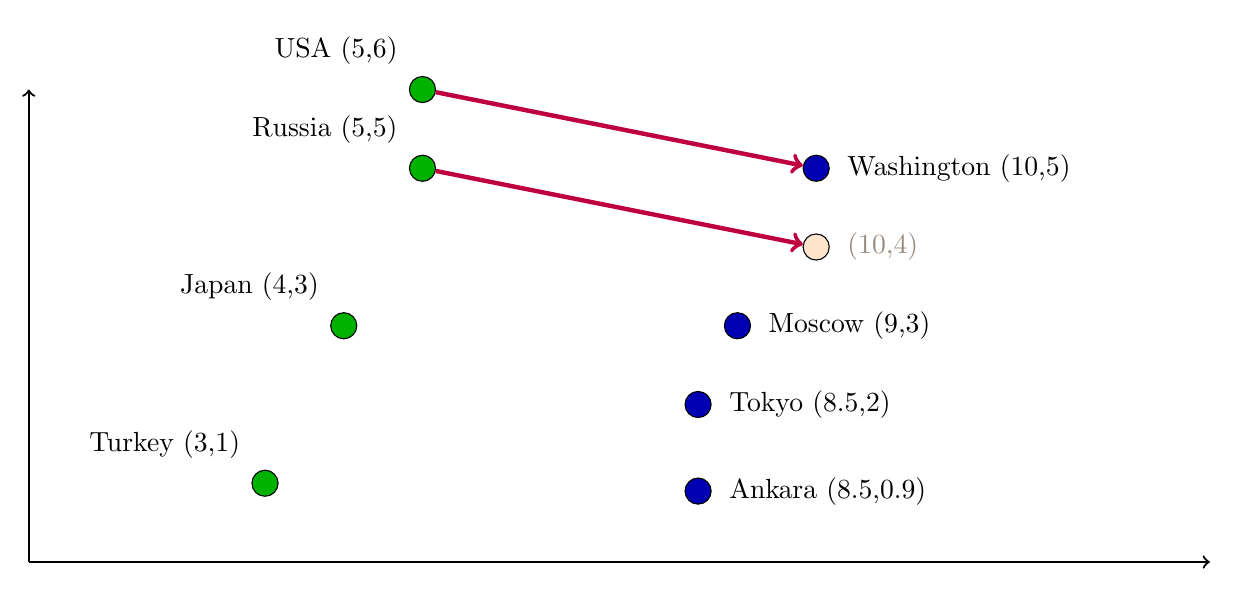
\begin{tikzpicture}
      \draw[->,thick] (0,0) -- (15, 0);
      \draw[->,thick] (0,0) -- (0, 6);
      \node[draw,circle,fill=green!70!black] (usa) at (5, 6) {};
      \node[draw,circle,fill=green!70!black] (russia) at (5, 5) {};
      \node[draw,circle,fill=green!70!black] (japan) at (4, 3) {};
      \node[draw,circle,fill=green!70!black] (turkey) at (3, 1) {};
      \node[draw,circle,fill=blue!70!black] (washington) at (10, 5) {};
      \node[draw,circle,fill=orange!20] (moscow_pred) at (10, 4) {};
      \node[draw,circle,fill=blue!70!black] (moscow) at (9, 3) {};
      \node[draw,circle,fill=blue!70!black] (tokyo) at (8.5, 2) {};
      \node[draw,circle,fill=blue!70!black] (ankara) at (8.5, 0.9) {};
      % Countries.
      \node[above left=1mm of usa] {USA (5,6)};
      \node[above left=1mm of russia] {Russia (5,5)};
      \node[above left=1mm of japan] {Japan (4,3)};
      \node[above left=1mm of turkey] {Turkey (3,1)};
      % Capitals.
      \node[right=1mm of washington] {Washington (10,5)};
      \node[right=1mm of moscow_pred] {\color{orange!20!black!50} (10,4)};
      \node[right=1mm of moscow] {Moscow (9,3)};
      \node[right=1mm of tokyo] {Tokyo (8.5,2)};
      \node[right=1mm of ankara] {Ankara (8.5,0.9)};
      % Relations
      \draw[->,ultra thick, purple] (usa) -- (washington);
      \draw[->,ultra thick, purple] (russia) -- (moscow_pred);
    \end{tikzpicture}
  \end{center}
  \caption{From \href{https://papers.nips.cc/paper/2013/file/9aa42b31882ec039965f3c4923ce901b-Paper.pdf}{Mikolov et. al. ``Distributed Representations of Words and Phrases and their Compositionality''}: in this representation, the vector between capitals Washington and USA is given by $[\texttt{Washington} - \texttt{USA}] = [5, -1]$. The easiest way to predict the capital of Russia is to simply take $\texttt{Russia} + [5, -1] = [10, 4]$. Because there are no cities with that representation, we'll search for the capital city that is most similar by comparing each vector with the Euclidean distances (or Cosine similarities). The catch is that we need a vector space where the representations capture the relative meaning of words.}
\end{figure}

\subsection{Principal Components Analysis}
\paragraph{Visualization and PCA} Often, we'll have vector representations in very high dimension, but we'll want to find a way to reduce the dimensions of the vectors to two dimensions so that we may plot it on a 2-D cartesian plane. What's the intuition? Principal Component Analysis is they key: it allows us to take a representation with $d > 2$ dimensions and project it down to a lower dimension, e.g. $d=2$, which we can then plot. If you perform PCA on your data, you might find that your word representation captures relationship between pairs of words that you expect to be related, in so far as these related words appear in clusters within the plot; you can confirm known relationships and also spot new ones using this technique.

\begin{minipage}{1.0\textwidth}
  \begin{multicols}{3}
  \begin{tikzpicture}[
    declare function={a(\x)=1;},
    declare     function={b(\x)=0;}
  ]
  \begin{axis}[
    domain=1:4,
    axis lines=middle,
    axis equal image,
    xtick=\empty,
    ytick=\empty,
    enlargelimits=true,
    clip mode=individual,
    clip=false
  ]
  \addplot [orange, only marks, mark=x, samples=20, mark size=2]         {x*0.5*(a(x)+b(x)) + 0.5*rand*(a(x)-b(x))};
  \node at (0, -1) {};
\end{axis}
\node at (4, 1) {Correlated data};
\end{tikzpicture}
\vfill\null \columnbreak
\begin{tikzpicture}
  \draw[->] (1.5,-0.3) -- (5, -0.3);
  \draw[->] (1.5,-0.3) -- (1.5, 1.8);
  \node at (4, 4) {};
  \node at (2.75, 2) {\small Un-correlated Features};
  \draw (1.7, -0.3) node[cross,rotate=30,color=orange] {};
  \draw (2.0, -0.4) node[cross,rotate=30,color=orange] {};
  \draw (2.3, +0.1) node[cross,rotate=30,color=orange] {};
  \draw (2.6, +0.2) node[cross,rotate=30,color=orange] {};
  \draw (2.9, -1.37) node[cross,rotate=30,color=orange] {};
  \draw (3.2, +0.15) node[cross,rotate=30,color=orange] {};
  \draw (3.5, -1.50) node[cross,rotate=30,color=orange] {};
  \draw (3.8, -1.35) node[cross,rotate=30,color=orange] {};
  \draw (4.1, +0.05) node[cross,rotate=30,color=orange] {};
  \draw (4.4, -0.45) node[cross,rotate=30,color=orange] {};
  \draw (4.7, -0.27) node[cross,rotate=30,color=orange] {};
\end{tikzpicture}
\vfill\null \columnbreak
\begin{tikzpicture}
  \draw[->] (1.5,-0.3) -- (5, -0.3);
  \draw[->] (1.5,-0.3) -- (1.5, 1.8);
  \node at (4, 4) {};
  \node at (2.75, 2) {\small Dimensionality Reduction};
  % Original points.
  \draw (1.7, -0.3) node[cross,rotate=30,color=orange!30] (n1) {};
  \draw (1.8, -0.4) node[cross,rotate=30,color=orange!30] (n2) {};
  \draw (2.3, +0.1) node[cross,rotate=30,color=orange!30] (n3) {};
  \draw (2.4, +0.2) node[cross,rotate=30,color=orange!30] (n4) {};
  \draw (2.9, -1.37) node[cross,rotate=30,color=orange!30] (n5)  {};
  \draw (3.2, +0.15) node[cross,rotate=30,color=orange!30] (n6)  {};
  \draw (3.3, -1.50) node[cross,rotate=30,color=orange!30] (n7)  {};
  \draw (3.4, -1.35) node[cross,rotate=30,color=orange!30] (n8)  {};
  \draw (4.1, +0.05) node[cross,rotate=30,color=orange!30] (n9)  {};
  \draw (4.15, -0.45) node[cross,rotate=30,color=orange!30] (n10)  {};
  \draw (4.7, -0.27) node[cross,rotate=30,color=orange!30] (n11)  {};
  % Projected.
  \draw (1.7, -0.3) node[cross,rotate=30,color=orange] (p1) {};
  \draw (1.8, -0.3) node[cross,rotate=30,color=orange] (p2) {};
  \draw (2.3, -0.3) node[cross,rotate=30,color=orange] (p3) {};
  \draw (2.4, -0.3) node[cross,rotate=30,color=orange] (p4) {};
  \draw (2.9, -0.3) node[cross,rotate=30,color=orange] (p5)  {};
  \draw (3.2, -0.3) node[cross,rotate=30,color=orange] (p6)  {};
  \draw (3.3, -0.3) node[cross,rotate=30,color=orange] (p7)  {};
  \draw (3.4, -0.3) node[cross,rotate=30,color=orange] (p8)  {};
  \draw (4.1, -0.3) node[cross,rotate=30,color=orange] (p9)  {};
  \draw (4.15, -0.3) node[cross,rotate=30,color=orange] (p10)  {};
  \draw (4.7, -0.3) node[cross,rotate=30,color=orange] (p11)  {};
  \draw[dashed] (n1) -- (p1);
  \draw[dashed] (n2) -- (p2);
  \draw[dashed] (n3) -- (p3);
  \draw[dashed] (n4) -- (p4);
  \draw[dashed] (n5) -- (p5);
  \draw[dashed] (n6) -- (p6);
  \draw[dashed] (n7) -- (p7);
  \draw[dashed] (n8) -- (p8);
  \draw[dashed] (n9) -- (p9);
  \draw[dashed] (n10) -- (p10);
  \draw[dashed] (n11) -- (p11);
\end{tikzpicture}
\end{multicols}
\end{minipage}
Using PCA, we first find a set of uncorrelated features. Then, we can project our data into a lower dimensional space, trying to retain as much information as possible.

\paragraph{PCA algorithm} How do we get uncorrelated features? Realize that the eigenvectors of the covariance matrix of our data correspond to the uncorrelated features for our data, and the eigenvalue corresponds to the amount of information retained by each feature. Note that it's essential that our eigenvectors are sorted according to their eigenvalues from largest to smallest (in magnitude): this means that if we use the first $k$ eigenvectors to get a representation we are greedily selecting vectors that retain the most information from our data.

\begin{enumerate}
\item Mean-normalize data: $x_i = \frac{x_i - \mu_{x_i}}{\sigma_{x_i}}$.
\item Obtain covariance matrix $\Sigma$.
\item Perform Singular Value Decomposition on $\Sigma$ to get three matrices, where the first stores the eigenvectors $U$ (columnwise), the second $S$ stores the eigenvalues along the diagonal.
\item Dot produt to Project your data: $X' = XU[:, 0:k]$, where $k$ is the   number of dimensions we wish to reduce to.
\item Calculate Percentage of Retained Variance: $\frac{\sum_{i=0}^{k-1} S_{ii}}{\sum_{j=0}^{d-1} S_{jj}}$.
\end{enumerate}
Eigenvectors give the direction of uncorrelated features, whereas the eigenvalues are the variance of the new features. The dot product gives the projection on uncorrelated features.

\section{Machine Translation}\vspace{.1pt} \hrule height 2pt \smallskip \renewcommand{\arraystretch}{1}% Tighter
\subsection{Transforming Word Vectors}
Word vectors can capture important properties of words. Let's make use of them to learn to align words into different languages, which will give us a basic translation program; locality sensitive hashing will speed it up.

\paragraph{Overview of translation}
In order to translate an English word to a French word, one naive way could be to generate an extensive list of English words and their associated French word. If you ask a human to do this, you would find someone who knows both languages to start making a list. If, however, you want a machine to do this, you need to first calculate word embeddings associated with English and word embeddings associated with French. Next, retrieve the English word embedding of a particular English word such as ``cats'', then find some way to transform the English word embedding into word embedding that has a meaning in the French word vector space; we'll see how to convert between vector spaces in a moment. The next step is to search for word vectors in the French word vector space that are most similar to the transformed vector representation: the most similar words are candidate words for our translation.

\paragraph{Transforming vectors using matrices} Define a randomly selected matrix $R$ and see how well it works to transform our English vector space representation $X$ into our French vector space representation $Y$, i.e. compute $XR \approx Y$. In order for this to work, you'll need to first get a subset of English words and their French equivalence, get the respective word vectors, and stack the word vectors in their respective matrices $X$ and $Y$. They key is to keep the rows lined up (or to align the row vectors): i.e. if the first row of the English matrix $X$ contains the word representation for ``cat'', then so should the French matrix $Y$ contain the word representation for the translated word. It's natural at this point to ask: if we already have the mappings from $X \leadsto Y$ (i.e. the translation pairs), then why not just store them in an associative data-structure like a dictionary...why train a model at all? The nice property of our transformation matrix $R$ is that it will \emph{generalize} to translate unseen example inputs. So, we only need to train on a subset of the English-French vocabulary, and \emph{not} the entire vocabulary.

\paragraph{Finding a good transformation matrix} We define our loss function as
\[
  \texttt{Loss} = \|XR - Y\|_F.
\]
where $\|A\|_F = \sqrt{\sum_{i=1}^m \sum_{j=1}^n |A_{ij}|^2}$.
If we start with a random matrix $R$, we can gradually improve upon it in an iterative fashion. We first compute the gradient by taking the gradient of the loss function with respect to matrix $R$, i.e. $g = \frac{\partial}{\partial R}\texttt{Loss}$, then update using gradient descent, i.e. $R \gets R - \alpha g$. We can either pick a fixed number of times to go through the loop, or exit the loop when the loss falls below a certain threshold. In practice, it's easier to minimize the the square of the norm instead. What about the gradient of the loss function, which is defined as the derivative of the loss with respect to the matrix $R$. With our loss:
\[
  g = \frac{\partial}{\partial R} \texttt{Loss} = \frac{2}{m} \left(X^T(XR - Y)\right),
\]
where $m$ is the number of rows in our training matrix.

\subsection{Approximate $k$-nearest neighbors and Locality Sensitive Hashing}
\paragraph{Finding k-nearest neighbors of a vector} In the context of Machine Translation, notice that the transformed word vector after the transformation of its embedding through a matrix $R$ would be in the French vector space, but! it's not going to be identically equal to any of the word vectors in the French vector space. We need to search through the French word vectors to find a French word that is similar to the one we created from the transformation.

To solve this problem, let's look at a related problem: how do you find your friends who are living nearby? One way to do this is to go through your address book and for each friend, get their addres, and calculate how far away they are from our hometown of San Francisco. We then sort our friends according to their distance from San Francisco. Notice that if we have a lot of friends, this is a time intensive process. A more efficient way is to observe that, if it were somehow possible to \emph{filter} our friends list to only those who live in the same continent, for example, then we could cut down our search space drastically. When you think about organizing subsets of a dataset efficiently, you might think about placing your data into buckets. If you think about buckets, then you'll definitely want to think about hash-tables.

\paragraph{Hash tables} Let's say we have several data items and we want to group them into buckets by some kind of similarity. One bucket can hold more than one item and each item is always assigned to the same bucket.

\begin{figure}[h]
\begin{center}
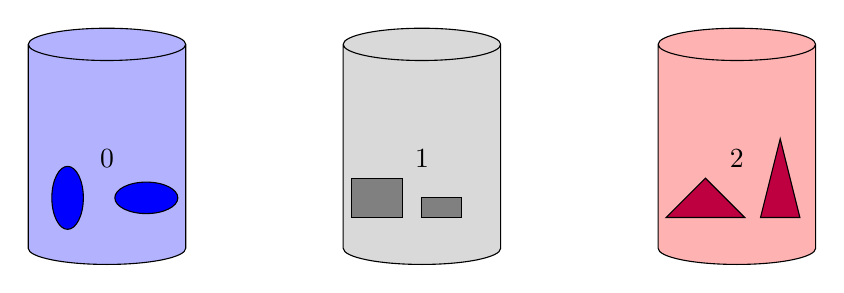
\begin{tikzpicture}[>=latex,shorten >=2pt,shorten <=2pt,shape aspect=1]
\node (A) at (0, 0) [cylinder, shape border rotate=90, draw,minimum height=3cm,minimum width=2cm,fill=blue!30]
{0};
\draw[fill=blue,scale=2] (-0.25,-0.25) ellipse (1mm and 2mm);
\draw[fill=blue,scale=2] (+0.25,-0.25) ellipse (2mm and 1mm);
\node (B) at (4, 0) [cylinder, shape border rotate=90, draw,minimum height=3cm,minimum width=2cm,fill=gray!30]
{1};
\draw[fill=gray] (+3.10,-0.75) rectangle (3.75, -0.25);
\draw[fill=gray] (+4,-0.75) rectangle (4.5, -0.5);
\node (C) at (8, 0) [cylinder, shape border rotate=90, draw,minimum height=3cm,minimum width=2cm,fill=red!30]
{2};
\draw[fill=purple] (7.1, -0.75) -- (7.6, -0.25) -- (8.1, -0.75) -- cycle;
\draw[fill=purple] (8.3, -0.75) -- (8.55, +0.25) -- (8.8, -0.75) -- cycle;
\end{tikzpicture}
\end{center}
\caption{Here's one pictorial example of hash buckets. One bucket might end up storing blue ovals, another might store gray rectangles, and a third may store magenta triangles.}
\end{figure}

How can we do this with word vectors? Let's first assume that word vectors have 1-dimension instead of several hundred. So, each word is represented by a \emph{single} scalar value. We need to figure out a mapping from values to hash buckets, i.e.
\[
  \texttt{HashFunction}(\textrm{vector}) \longrightarrow \textrm{Hash Value}.
\]

A function that assigns a hash value is called a hash function.

\begin{figure}
  \begin{center}
    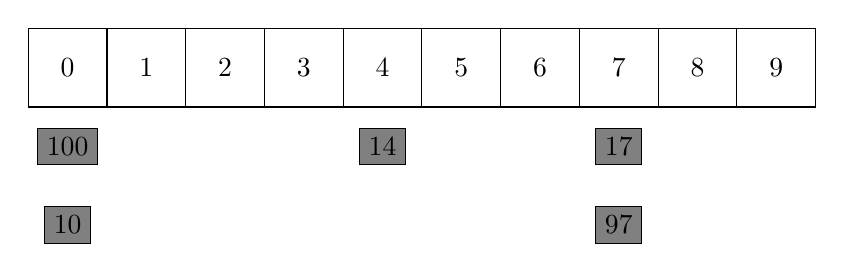
\begin{tikzpicture}
      \draw (0,0) grid (10, 1);
      \foreach \x in {0.5, 1.5, ..., 9.5} {
        \node at (\x, 0.5) {\pgfmathparse{int(\x-0.5)}\pgfmathresult};
      }
      \node[draw,rectangle,fill=gray] at (0.5, -0.5) {100};
      \node[draw,rectangle,fill=gray] at (0.5, -1.5) {10};
      \node[draw,rectangle,fill=gray] at (4.5, -0.5) {14};
      \node[draw,rectangle,fill=gray] at (7.5, -0.5) {17};
      \node[draw,rectangle,fill=gray] at (7.5, -1.5) {97};
    \end{tikzpicture}
  \end{center}
  \caption{One example could be, in our context of a 1-D embedding, to take the value modulo ten and assign it to one of ten buckets $\{0,1,\ldots,9\}$.}
\end{figure}

To build this example out in code, we simply define

\begin{python}
def basic_hash_table(value_l, n_buckets):
  def hash_function(value_l, n_buckets):
    return int(value) % n_buckets
  hash_table = {i:[] for i in range(n_buckets)}
  for value in value_l:
    hash_value = hash_function(value, n_buckets)
    hash_table[hash_value].append(value)
  return hash_table
\end{python}

Notice that in our \texttt{hash\_function()} definition, we are using a \emph{dictionary}-comprehension, where we are associating integer keys with empty lists as value; this initializes our hash-table. Now, realize that our original goal was to place similar word vectors into the \emph{same} bucket. In the example above, it doesn't look like numbers that are close to each other are in the same bucket, e.g. 10, 14, and 17 are all in different buckets. Idealy, we want a hash function that places similar word vectors in the same bucket; this brings us to locality sensitive hashing. Locality is another word for location, and sensitive is another word for caring. So locality sensitive hashing is a hashing method that cares very deeply about assigning items based on where they're located in vector space.

\begin{figure}[h]
  \begin{center}
    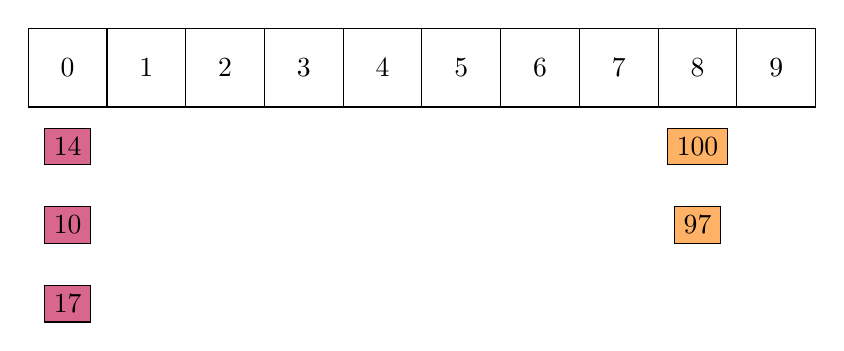
\begin{tikzpicture}
      \draw (0,0) grid (10, 1);
      \foreach \x in {0.5, 1.5, ..., 9.5} {
        \node at (\x, 0.5) {\pgfmathparse{int(\x-0.5)}\pgfmathresult};
      }
      \node[draw,rectangle,fill=purple!60] at (0.5, -0.5) {14};
      \node[draw,rectangle,fill=purple!60] at (0.5, -1.5) {10};
      \node[draw,rectangle,fill=purple!60] at (0.5, -2.5) {17};
      \node[draw,rectangle,fill=orange!60] at (8.5, -0.5) {100};
      \node[draw,rectangle,fill=orange!60] at (8.5, -1.5) {97};
    \end{tikzpicture}
  \end{center}
  \caption{A good hash-function places similar word vectors in the same bucket.}
\end{figure}

\paragraph{Locality sensitive hashing} A key method for reducing the computational cost of finding $k$-nearest neighbors in high-dimensional spaces is locality-sensitive hashing. Let's start with examples of word vectors with two dimensions.

\begin{figure}
  \begin{center}
    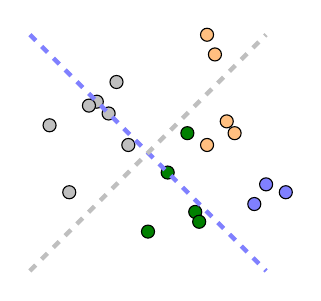
\begin{tikzpicture}[scale=5]
      % Gray nodes.
      \node[draw,circle,fill=gray!50,scale=0.5] at (-0.2, -0.1) {};
      \node[draw,circle,fill=gray!50,scale=0.5] at (-0.25, 0.07) {};
      \node[draw,circle,fill=gray!50,scale=0.5] at (-0.05, 0.02) {};
      \node[draw,circle,fill=gray!50,scale=0.5] at (-0.10, 0.10) {};
      \node[draw,circle,fill=gray!50,scale=0.5] at (-0.13, 0.13) {};
      \node[draw,circle,fill=gray!50,scale=0.5] at (-0.08, 0.18) {};
      \node[draw,circle,fill=gray!50,scale=0.5] at (-0.15, 0.12) {};
      % Green nodes.
      \node[draw,circle,fill=green!50!black,scale=0.5] at (0.00, -0.20) {};
      \node[draw,circle,fill=green!50!black,scale=0.5] at (0.05, -0.05) {};
      \node[draw,circle,fill=green!50!black,scale=0.5] at (0.10, +0.05) {};
      \node[draw,circle,fill=green!50!black,scale=0.5] at (0.12, -0.15) {};
      \node[draw,circle,fill=green!50!black,scale=0.5] at (0.13, -0.175) {};
      % Orange nodes.
      \node[draw,circle,fill=orange!50,scale=0.5] at (+0.15, 0.02) {};
      \node[draw,circle,fill=orange!50,scale=0.5] at (+0.20, 0.08) {};
      \node[draw,circle,fill=orange!50,scale=0.5] at (+0.22, 0.05) {};
      \node[draw,circle,fill=orange!50,scale=0.5] at (+0.17, 0.25) {};
      \node[draw,circle,fill=orange!50,scale=0.5] at (+0.15, 0.30) {};
      % Blue nodes.
      \node[draw,circle,fill=blue!50,scale=0.5] at (+0.30, -0.08) {};
      \node[draw,circle,fill=blue!50,scale=0.5] at (+0.35, -0.10) {};
      \node[draw,circle,fill=blue!50,scale=0.5] at (+0.27, -0.13) {};
      % Plands
      \draw[-,dashed,ultra thick, blue!50] (-0.3,0.3) -- (0.3,-0.3);
      \draw[-,dashed,ultra thick, gray!50] (-0.3,-0.3) -- (0.3,0.3);
    \end{tikzpicture}
  \end{center}
  \caption{Let's say you want to find a way to know that these blue dots are somehow close to each other, and that these gray dots are also related to each other. First, divide the space using dashed lines, called \emph{planes}. Notice that the blue plane slices up the space into vectors that are above it or below it, where the blue bectors all happens to be on the same side of the blue plane. Similarly, the gray vectors all lie above the gray plane. It looks like the planes can help us bucket the vectors into subsets based on their location, which is exactly what we want: a hashing function that is sensitive to the location of the items that it's assigning into buckets.}
\end{figure}

\begin{figure}
  \begin{center}
    \begin{tikzpicture}
      \draw[<->,gray] (-2, 0) -- (2, 0);
      \draw[<->,gray] (0, -2) -- (0, 2);
      \draw[-,dashed,gray] (-2,+2) -- (2,-2);
      \draw[->,thick,blue!80] (0,0) -- (1,-1);
      \draw[->,thick,orange!80] (0,0) -- (-1.5, 1.5);
      \draw[->,thick,purple!80] (0,0) -- (1, 1);
    \end{tikzpicture}
  \end{center}
  \caption{A plane can be visualized in 2-D space by a dashed gray line. It actually represents all possible vectors that would be sitting on that plane, i.e. the orange and blue vectors that are parallel to the plane. You can define a plane with a single vector. The magenta vector is perpendicular to the plane, and it's called the normal vector to that plane: it is perpendicular to any vectors that lie on the plane.}
\end{figure}

\begin{figure}
  \begin{center}
    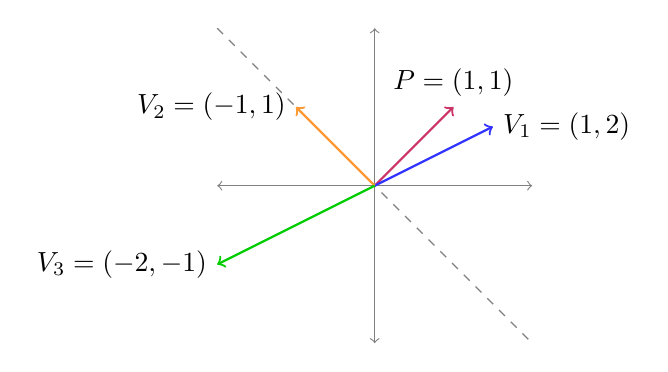
\begin{tikzpicture}
      \draw[<->,gray] (-2, 0) -- (2, 0);
      \draw[<->,gray] (0, -2) -- (0, 2);
      \draw[-,dashed,gray] (-2,+2) -- (2,-2);
      \draw[->,thick,purple!80] (0,0) -- (1, 1) node[above] {\color{black} $P = (1, 1)$};
      \draw[->,thick,blue!80] (0,0) -- (1.5, 0.75) node[right] {\color{black} $V_1 = (1, 2)$};
      \draw[->,thick,orange!80] (0,0) -- (-1, 1) node[left] {\color{black} $V_2         = (-1, 1)$};
      \draw[->,thick,green!80!black] (0,0) -- (-2, -1) node[left] {\color{black} $V_3         = (-2, -1)$};
    \end{tikzpicture}
  \end{center}
  \caption{Consider three sample vectors in blue, orange, and green. The normal vector to the plane is labeled $P$. Let's focus on vector $V_1$: observe that the inner product $\langle P, V_1 \rangle = 3$. Similarly, $\langle P, V_2 \rangle = 0$, and $\langle P, V_3 \rangle = -3$. Realize that when the inner product is positive with the normal vector, the vector is on one side of the plane, and if the inner product is negative it's on the opposite side of the plane. If the dot product is zero, the vector is on the plane.}
\end{figure}

\paragraph{Visualizing a dot product} Let's visualize the dot product further.
\newpage
\begin{figure}
  \begin{center}
    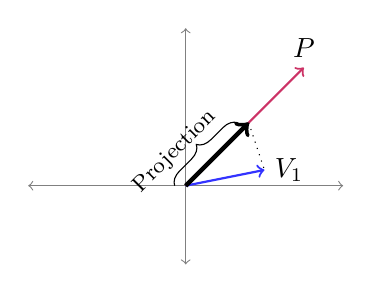
\begin{tikzpicture}
      \draw[<->,gray] (-2, 0) -- (2, 0);
      \draw[<->,gray] (0, -1) -- (0, 2);
      \draw[->,thick,purple!80] (0,0) -- (1.5, 1.5) node[above] {\color{black} $P$};
      \draw[->,thick,blue!80] (0,0) -- (1, 0.2) node[right] {\color{black}                 $V_1$};
      \draw[-,dotted] (0.8, 0.8) -- (1, 0.2);
      \draw[->,ultra thick] (0,0) -- (0.8,0.8);
      \draw [decorate,decoration={brace,amplitude=5pt},xshift=-4pt,yshift=0pt]
(0,0) -- (0.8,0.8) node [black,midway,xshift=-0.4cm,yshift=1pt,rotate=45] 
{\footnotesize Projection};
    \end{tikzpicture}
  \end{center}
  \caption{To visualize the dot product, imagine one of the vectors such as $P$, as if it's the surface of the Earth. Gravity pulls all objects \emph{straight} down towards the surface of the Earth. Next, pretend you're standing at the end of the vector $V_1$. You tie a string to a rock and let gravity pull the rock to the surface of vector $P$: the string is prependicular to vector $P$. Now, if you draw a vector that's in the same direction of $P$ but ends up at the rock, you'll have what's called the \emph{projection} of vector $V_1$ onto vector $P$. The magnitude or length of that vector is equal to the dot product of $V_1$ and $P$, i.e. $\|PV_1^T\|$. The sign of the dot product indicates the direction with respect to the purple normal vector: a positve sign indicates a vector is pointed in the same direction, whereas a negative sign means they are pointed in opposite directions.}
\end{figure}

We can implement a simple Python function to determine whether a vector $v$ is pointed in the same or oppositive direction of a normal vector $P$:

\begin{python}
def side_of_plane(P,v):
  dotproduct = np.dot(P, v.T)
  sign_of_dot_product = np.sign(dotproduct)
  sign_of_dot_product_scalar = np.asscalar(sign_of_dot_product)
  return sign_of_dot_product_scalar
\end{python}

We first compute the inner product, then examine the sign, then convert the sign to a one, zero, or minus one depending on whether the inner product is positive, zero, or negative.

\paragraph{Multiple planes} How can we combine information from multiple planes into a single hash value? Previously, we saw how we can examine the sign of the dot product between the normal vector of a plane and a vector representing our data, and we could get a notion of position relative to the plane. Here, we're going to examine how to use information from multiple planes in order to get a single hash value for your data in your vector space, since in order to divide your vector space into manageable regions, you'll want to use more than one plane.

\begin{itemize}
\item For each plane, find out whether a vector is on the positive or negative side of that plane: you'll get multiple signals, one for each plane and we need to find a way to combine them all into a single hash value. I.e. compute $P V_i^T \leadsto \textrm{sign}_i \leadsto h_i$ where $h_i \in \{0,1\}$ according to $h_i = \mathbbm 1_{\textrm{sign}_i \geq 0}$, indicating the side of the plane that the vector lies on.
\item Compute $\texttt{hash} = \sum_{j=1} h_j 2^{j-1}$.
\end{itemize}

\begin{python}
def hash_multiple_plane(P_l, v):
  hash_value = 0
  for i, P in enumerate(P_l):
    sign = side_of_plane(P, v)
    hash_i = 1 if sign >= 0 else 0
    hash_value += 2**i * hash_i
  return hash_value
\end{python}

\paragraph{Approximate $k$-nearest neighbors} Let's devise an algorithm that computes $k$-nearest neighbors much faster than brute search. We've seen how a few planes can help to divide a vector space into regions. But how do you know if a set of planes is the \emph{optimal} way to divide the vector space? You can't, so why not create multiple sets of random planes to divide up the vector space into multiple, independent sets of hash tables? This is akin to creating multiple copies of the universe, or a multiverse. You can make all of these different sets of random planes in order to help find a good set of $k$-nearest neighbors, as follows:
\begin{itemize}
\item Create multiple sets of planes, in parallel.
\item For each \emph{set} of planes, determine the neighbors i.e. the words that   are in the same hash-bucket as the word in question.

(Note that each set of planes will yield a different (possibly overlapping) set of neighbors)
\end{itemize}
By using multiple sets of random planes for locality-sensitive hashing, you have a more robust way of searching the vector space for a set of vectors that are possible candidates to be nearest neighbors. This technique is known as \emph{approximate} nearest neighbors because you're not searching the entire vector space, but just a subset of it. So the output is not the absolute $k$-nearest neighbors, but it's approximately the $k$k-nearest neighbors. We sacrifice precision in order to gain efficiency in our search.

How can we do this in code?

\begin{python}
num_dimensions = 2
num_planes = 3
random_planes_matrix = np.random.normal(size = (num_planes, num_dimensions))
v = np.array([[2,2]]);
def side_of_plane_matrix(P,v):
  dotproduct = np.dot(P, v.T)
  sign_of_dot_product = np.sign(dotproduct)
  return sign_of_dot_product

num_planes_matrix = side_of_plan_matrix(random_planes_matrix, v)
\end{python}

\paragraph{Searching documents} How can we use approximate $k$-nearest neighbors to search for pieces of text related to a query in a large collection of documents? We simply create vectors for both and find the nearest neighbors. In order to get ready to perform document search, we need to think through how to represent documents as vectors, instead of just words as vectors. Let's say you have a document composed of three words: ``I love learning''. How can we represent the entire document as a vector? We could find the word vectors for each individual word, and then simply add them together; in this case the resulting document vector has the same dimension as the word vector representation. Let's code this up:

\begin{python}
word_embedding = {'I': np.array([1, 1, 1]), 'love': np.array([-1, 0, 1]), 'learning': np.array([1,0,1])}
words_in_document = ['I', 'love', 'learning']
document_embedding = np.array([0, 0, 0])
for word in words_in_document:
  document_embedding += word_embedding.get(word, 0)

print(document_embedding)
\end{python}

Reference: \href{https://www.amazon.com/Speech-Language-Processing-Daniel-Jurafsky-ebook-dp-B00XIGSJQK/dp/B00XIGSJQK/ref=mt_kindle?_encoding=UTF8&me=&qid=1591993888}{``Speech   and Language Processing'' by Jurafsky, Martin, Norvig, and Russell}.

\section{Autocorrect and Minimum Edit Distance}\vspace{.1pt} \hrule height 2pt \smallskip \renewcommand{\arraystretch}{1}% Tighter
\subsection{Autocorrect} What is autocorrect exactly? It can mean slightly different things depending on the context. A key concept in performing autocorrect is quantifying how far apart two strings are, and calculating the minimum number of characters needed to be changed to go from one string to another.
\paragraph{What is autocorrect?} It changes misspelled into the correct ones. E.g.
\[
  \texttt{Happy birthday {\color{red} deah} friend!} \leadsto \texttt{Happy birthday {\color{green!80!black} dear} frend!}
\]
But what if we typed ``deer'' instead of ``deah'' or ``dear'': the word might be spelled correctly, but its context is incorrect. This is a more sophisticated problem that we will revisit later; for now, let's focus on \emph{misspelled} words.
\begin{enumerate}
\item Identify a misspelled word.
\item Find strings $n$ edit distance away: a string that is 1-edit distance away might be more likely to be a correct replacement than a string that is 2-edit distance away.
\item Filter candidates - only retain real words that are spelled correctly.
\item Calculate word probabilities - this informs us how likely each word is to appear in the context; we choose the most likely candidate as our replacement.
\end{enumerate}

\paragraph{Identify a misspelled word} How do we know that a word is misspelled? Well, if it's spelled correctly, we could look it up in a dictionary; otherwise, it's probably a misspelled word.
\begin{python}
if word not in vocab:
  misspelled = True
\end{python}
If a word is not in a dictionary, we flag it for correction. Recall that we've limited our focus to just spelling errors, not contextual errors. There are more sophisticated techniques for identifying words that are probably incorrect by looking at neighboring words, but for now, identifying a word as incorrect by its apparent misspelling will yield a powerful model that works well.\footnote{We conceded this means a word like ``deer'' in our introductory   example would not be flagged by this autocorrect program.}

\paragraph{Find strings $n$-edit distance away} An edit is a type of operation performed on a string to change it into another string. Edit distance counts the number of these operations, so that the $n$-edit distance metric tells us how far away one string is from another.
\begin{itemize}
  \item Consider an \emph{insert} operation, which adds a letter to a string at any position. E.g. if we take ``to'' and insert a ``p'' at the end we get ``top'', or if we insert a ``w'' in the middle we get ``two''.
\item We can also apply \emph{delete} operations, which remove a letter from a string. E.g. we can start with ``hat'' and delete single characters to yield ``ha'', ``at'', ``ht''.
\item There's also a \emph{swap} operation, which allows us to swap two adjacent letters. E.g. we can start with ``eta'' and swap to get ``eat'' or ``tea''. This does \emph{not} include switching two non-adjacent letters, i.e. a swap does not let us create ``ate'' by switching the ``e'' and the non-adjacent ``a'' in ``eta''.
\item We can also \emph{replace} one letter with another. E.g. ``jaw'' can be made into ``jar'' or ``paw''.
\end{itemize}

By combining these edits, we can finda list of all possible strings that are $n$-edits away from a given string. For auto-correct, $n$ is usually 1-3 edits.

\paragraph{Filter candidates} Notice how many of the strings generated don't look like actual words: to filter strings and keep real words we'll want to only consider correctly spelled words from our candidate list. We can again use a known dictionary to make comparisons against a known vocabulary.

\paragraph{Calculate probabilities} The final step is to calculate word probabilities and find the most likely word from the candidates. Consider an example sentence, ``I am happy because I am learning''.

\begin{table}[h]
  \begin{center}
  \begin{tabular}{c | c}
    \hline
    Word & Count \\
    \hline
    I & 2 \\
    am & 2 \\
    happy & 1 \\
    because & 1 \\
    learning & 1
  \end{tabular}
\caption{To calculate the probability of a word in a sentence, we need to calculate the word frequencies, and in addition the total number of words in the body of texts or corpus. The total number of (non-unique) words in the body of text or corpus is 7. Normally, a corpus would be much larger, e.g. all of the Harry Potter books. But for this pedagogical example, we consider our entire corpus to be this single sentence.}
\end{center}
\end{table}

For any word, we define the probability of its appearance $P(w)$ as
\[
P(w) = \frac{C(w)}{|V|},
\]
where $C(w)$ is the number of times the word appears, and $V$ is the total size of the corpus. For autocorrect, we simply find the word candidate with the highest probability and choose that word as the replacement.

\subsection{Minimum edit distance} Let's consider a slightly different problem: you're given two strings (possibly entire documents), and you want to evaluate how similar they are. Given one string, the minimum edit distance is the lowest number of operations needed to transform one string into the other.\footnote{Applications in NLP include spelling correction, document similarity, and machine translation.} For calculating minimum edit distance, we'll use three edit operations: insert (add a letter), delete (remove a letter), and replace (change 1 letter to another).

\begin{figure}[h]
  \begin{center}
    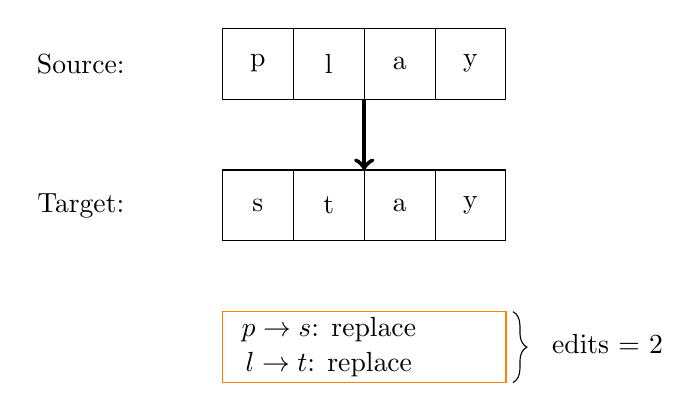
\begin{tikzpicture}[scale=0.9]
      \node at (-2, 0.5) {Source:};
      \draw (0, 0) grid (4, 1);
      \node at (0.5, 0.5) {p};
      \node at (1.5, 0.5) {l};
      \node at (2.5, 0.5) {a};
      \node at (3.5, 0.5) {y};
      \node at (-2, -1.5) {Target:};
      \draw (0, -2) grid (4, -1);
      \node at (0.5, -1.5) {s};
      \node at (1.5, -1.5) {t};
      \node at (2.5, -1.5) {a};
      \node at (3.5, -1.5) {y};
      \draw[->,ultra thick] (2, 0) -- (2, -1);
      \draw[orange] (0, -4) rectangle (4, -3);
      \draw [decorate,decoration={brace,amplitude=5pt},xshift=0pt,yshift=0pt]
      (4.1,-3) -- (4.1,-4) node [black,midway,xshift=1.2cm,yshift=1pt] {edits = 2};
      \node at (1.5, -3.25) {$p \to s$: replace};
      \node at (1.5, -3.75) {$l \to t$: replace};
    \end{tikzpicture}
  \end{center}
  \caption{In order to turn ``play'' into ``stay'', what is the minimum number of edits required? To turn ``p'' into ``s'', we need a replacement $p \leadsto s$, and to turn ``l'' into ``t'' we similarly need a replacement $l \leadsto t$. Both remaining characters are the same so we do nothing, and the total number of edits is now two.}
\end{figure}

Up until this point, we've treated all edit operations as having the same (unit-valued) cost. But now we'll consider different costs for different types of operations:

\begin{table}[h]
  \begin{center}
    \begin{tabular}{l c}
      Edit Cost: & \\
      \hline
      Insert & 1 \\
      Delete & 1 \\
      Replace & 2
    \end{tabular}
  \end{center}
  \caption{The above costs are intuitive if we think about a replace as a delete followed by an insert.}
\end{table}

But what about much longer strings and large corpora of texts or even DNA strings? You can try and solve these problems by brute force: adding one added distance at a time and enumerating all posibilities until one string changes to another; recognize that this requires exponential work with respect to the input string length. A much faster way is to use dynamic programming.

\subsubsection{Minimum edit distance algorithm}
We'll start by laying out the problem as follows.

\begin{figure}[h!]
  \begin{center}
    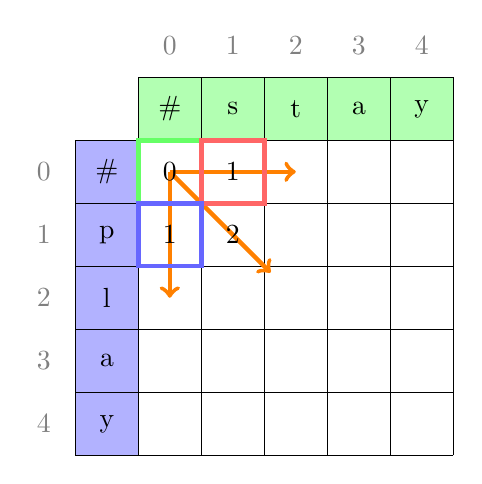
\begin{tikzpicture}[scale=0.8]
      \draw (0, 0) grid (5, 5);
      \draw[draw=black, fill=green!30] (0, 5) grid (5, 6) rectangle (0, 5);
      \draw[draw=black, fill=blue!30] (-1,0) grid (0,5) rectangle (-1, 0);
      \foreach \x in {0, 1, ..., 4} {
        \node at (\x+0.5, 6.5) {\color{gray} \x};
      }
      \node at (-1.5, 4.5) {\color{gray} 0};
      \node at (-1.5, 3.5) {\color{gray} 1};
      \node at (-1.5, 2.5) {\color{gray} 2};
      \node at (-1.5, 1.5) {\color{gray} 3};
      \node at (-1.5, 0.5) {\color{gray} 4};
      \node at (-0.5, 4.5) {\#};
      \node at (+0.5, 5.5) {\#};
      \node at (+1.5, 5.5) {s};
      \node at (+2.5, 5.5) {t};
      \node at (+3.5, 5.5) {a};
      \node at (+4.5, 5.5) {y};
      \node at (-0.5, 3.5) {p};
      \node at (-0.5, 2.5) {l};
      \node at (-0.5, 1.5) {a};
      \node at (-0.5, 0.5) {y};
      \draw[->,ultra thick, orange] (0.5, 4.5) -- (2.5, 4.5);
      \draw[->,ultra thick, orange] (0.5, 4.5) -- (2.1, 2.9);
      \draw[->,ultra thick, orange] (0.5, 4.5) -- (0.5, 2.5);
      \node at (0.5, 4.5) {0};
      \draw[ultra thick, green!60] (0, 4) rectangle (1, 5);
      \node at (1.5, 4.5) {1};
      \draw[ultra thick, red!60] (1, 4) rectangle (2, 5);
      \node at (0.5, 3.5) {1};
      \draw[ultra thick, blue!60] (0, 3) rectangle (1, 4);
      \node at (1.5, 3.5) {2};
    \end{tikzpicture}
  \end{center}
  \caption{The \# represents an empty string, and we've also set up row and column indices. If our table above is called $D$, we want the entries $D[i,j] = \textrm{source}[:i] \leadsto \textrm{target}[:j]$.}
\end{figure}

We've defined $D_{i,j}$ to represent the minimum edit distance between $\textrm{source}[:i]$ and $\textrm{target}[:j]$. If we have a source of length $m$ and a target of length $n$ then $D_{m,n}$ represents the minimum edit distance to transform one entire word to another. We'll compute this from the shortest substring to the full string. The intuition is that we can build upon each sub-problem by combining solutions, e.g. finding the minimum edit distance between two letters is easy. Then, we increase the problem size one letter at a time, building on what you already know.

\begin{itemize}
\item The first step is to transform the source empty string into the target empty string: this requires zero operations and so the edit distance is simply zero.
\item Now, we can move on to transforming our source ``p'' into an empty string,   which we can do with a single delete: edit distance is unit value.
\item We can also move on to transforming our source empty string to a target   ``s'', which we can do with a single insertion: edit distance is unit value.
\item Now, let's look at how to go from source ``p'' to target ``s'': there is more than one possible way to make this transformation. Each possible sequence of edits is known as a \emph{path}:
  \begin{itemize}
    \item starting with ``p'', you can insert ``s'' on the end to get ``ps'', then delete ``p'' from the beginning to get ``s''. This has a cost of one insert and one delete; notice that we've already calculated the cost of inserting a letter ``s'' as its given by the table entry above (in red) that we've already filled in. So, we actually just calculate the cost of deleting the ``p'' and add it onto the cost that you've stored in the red box above, which is $1+1 = 2$.
    \item starting with ``p'', we can delete ``p'' to get hashtag (empty string) and then insert ``s'' to get ``s''. Notice again that we've already calculated the cost of deleting ``p'' (in blue) to the left: the blue box is the cost of going from ``p'' to hashtag (empty string) by deleting ``p'', so we can calculate the cost of inserting ``s'' and add it to the cost that you've stored in the blue box on the left. This is $1 + 1 = 2$.
\item The third way is to replace ``p'' with ``s'' with a replacement, which has cost 2. We can think of this as going from the green cell to the target cell.
\end{itemize}
\item Now, we take the minimum of all three of these paths which yields 2 in this case.
\end{itemize}

Realize that in order to fill in a cell, we need to know the values of the cells above, to the left, and adjacent upper-left. In doing so, we can benefit from calculations already performed. We can We can generalize this to a formula such that we can fill in the entire table; but first, we must fill in the first row and first column in order to get the sufficient inputs to calculate the remaining entries.

\paragraph{Filling in first column:} this corresponds to transforming ``play'' into the empty string. We can use the following reccurrence relation:
\[
  D_{i,j} = D_{i-1,j} + \texttt{del\_cost}.
\]
I.e. we simply look at the cell above and add an extra delete edit. I.e. to make the string ``p'' into the empty string, we need one delete operation. To make ``pl'' into the empty string, we need to delete ``p'' and ``l'', which are two delete operations, and so on. Now, at $D_{4,0}$ we have the minimum edit distance for ``play'' to be transformed into the empty string, which is of course simply given by four deletions with a cost of four.

\paragraph{Filling in first row:} this corresponds to transforming the empty string into ``stay''. We can use the following, slightly different reccurrence relation:
\[
  D_{i,j} = D_{i,j-1} + \texttt{ins\_cost}.
\]
I.e. we simply look at the cell to the left and add an extra insertion edit.

\paragraph{Generalized dynamic programming formula for minimum edit distance} There is also a general formula for filling in each entry of our table

\[
  D_{i,j} = \min \begin{cases}
    D_{i-1, j} + \texttt{del\_cost} \\
    D_{i, j-1} + \texttt{ins\_cost} \\
    D_{i-1,j-1} + \mathbbm 1_{\texttt{src[i]} \neq \texttt{tar[j]}} \times \texttt{rep\_cost}
  \end{cases}
\]

The first argument to the \texttt{min} operator corresponds to ``coming from the cell above'', whereas the second argument corresponds to ``coming from the cell to the left'', and finally if you come from the cell to the upper-left then you do one of two things: either (i) add the replacement cost if the two corresponding letters between source and target don't match, or (ii) add nothing if they do (because there is no edit to be done for letters that are already the same).\footnote{It can be interesting to color the table according to the magnitude of the edit distances in the cells. This can reveal some interesting patterns. In our example table, fours will lie along the diagonal beyond ``the middle'' of the table, because this corresponds to where the prefixes have been made the same and no more edits are to be made.}

\paragraph{Levenshtein distance and backtrace} We've been using \href{https://en.wikipedia.org/wiki/Levenshtein_distance#Definition}{Levenshtein distance metric}. Finding the minimum edit distance doesn't always solve the whole problem. Sometimes, we need to know how we got there as well: we can do this by storing a backtrace which is simply a pointer in each cell letting you know where you came from to get there. So, you know the path taken across the table from the top-left corner to the bottom right corner (i.e. how we transformed our string); this tells us the edits that were made and is particularly useful in problems dealing with string alignment. We lastly mention that our algorithm laid out in the last section is an example of dynamic programming: we solve the smallest subproblem first and then reuse that result to solve the next bigger subproblem, saving that result, and continuing on. This is a well known technique in computer science.

\section{Part of Speech Tagging}\vspace{.1pt} \hrule height 2pt \smallskip \renewcommand{\arraystretch}{1}% Tighter
\subsection{What is part of speech tagging?} Part of speech tagging refers to the category of words or the lexical terms in the language. E.g. in English, lexical terms include \texttt{noun, verb, adjective, adverb, pronoun, preposition}, and many others.

\begin{equation*}
\underset{\textrm{adverb}}{\textrm{Why}} \hspace{10pt}             \underset{\textrm{adverb}}{\textrm{not}} \hspace{10pt}
\underset{\textrm{verb}}{\textrm{learn}} \hspace{10pt}
\underset{\textrm{noun}}{\textrm{something}} \hspace{10pt}         
\underset{\substack{\textrm{punctuation} \\ \textrm{mark}}}{\textrm{?}}
\end{equation*}

We're going to use a short representation called \emph{tags} to represent these categories. The process of assigning these tags to the words of a sentence is referred to as parts of speech tagging.

\begin{table}[h]
\begin{center}
  \begin{tabular}{l | l | l}
    \hline
    \textbf{lexical term} & \textbf{tag} & \textbf{example} \\
    \hline
    noun & NN & something, nothing \\
    verb & VB & learn, study \\
    determiner & DT & the, a \\
    w-adverb & WRB & why, where \\
    $\ldots$ & & 
  \end{tabular}
\end{center}
\end{table}

Because parts of speech tags describe the characteristic structure of lexical terms in a sentence or text, we can use them to make assumptions about semantics. We can use them to identify named entities, e.g.
\begin{verbatim}
The Eiffel Tower is located in Paris.
\end{verbatim}
The terms ``Eiffel Tower'' and ``Paris'' are both named entities. Tags can also be used for co-reference resolution, i.e. if you have two sentences: ``the Eiffel Tower is located in Paris. \textbf{It} is 324 meters high.'' then we can use parts of speech tagging to infer that ``it'' refers in this context to the Eiffel tower. A last example is in speech recognition: we can use parts of speech tags to check if a sequence of words has a high probability or not.

\subsection{Markov Chains} Let's start with a small example with what we want to accomplish, and then let's see how Markov Chains can help accomplish our task. Suppose we are given a \emph{sentence prefix}, ``why not learn...'', and we want to predict whether the following word is more likely to be a noun rather than another verb. If you examine the word ``learn'', note that it's a verb. Being familiar with the English language, we might guess that if you see a verb in a sentence, then the following word is more likely to be a noun rather than another verb. The core idea here is that the likelihood of the next word's parts of speech tag in a sentence tends to depend (only) on the parts of speech tag of the previous word. We can represent the likelihoods visually:
\begin{figure}
  \begin{center}
    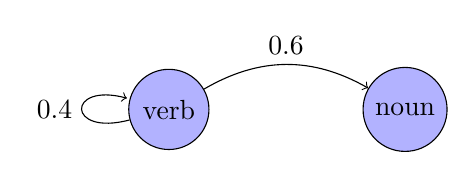
\begin{tikzpicture}
      \node[draw,circle,fill=blue!30] (verb) at (0, 0) {verb};
      \node[draw,circle,fill=blue!30] (noun) at (3, 0) {noun};
      \draw[->] (verb) edge[loop left] node {0.4} (verb);
      \draw[->] (verb) edge[bend left] node[above] {0.6} (noun);
    \end{tikzpicture}
    \caption{The nodes indicate states, and the arrows indicate transitions where the corresponding floating points values describe transition probabilities.}
  \end{center}
\end{figure}

\paragraph{Markov chains defined}
A Markov Chain is a type of stochastic model that describes a sequence of possible events, with the property that to get the probability for each event, we need only the state of the previous event! The word stochastic means random. A stochastic model incorporates and models processes that have a random component to them. Markov chains can always be depicted graphically as a directed graph with nodes and edges. I.e. a Markov chain is a graph of states and transitions between these states. The key property of a Markov chain is the Markov property: the probability of the next event only depends on the current events.


\paragraph{Intuition for Markov property}
The Markov property is what allows us to keep our model simple by saying that all you need to determine the next state is the current state information; we don't need any other information from any of the previous states. Going back to an analogy: suppose we consider whether water is in a solid, liquid, or gaseous state. If we look at a cup of water that is sitting outside, the current state of the water is a liquid state. When modeling the probability that the water in the cup will transition into the gas state, we don't need to know the previous history of the water: whether it previously came from ice cubes or from rain clouds is irrelevant!

\paragraph{Applying Markov chains to parts of speech tagging} Let's think about a sentence as a sequence of words with associated parts of speech tags. We can represent that sequence with a graph where the parts of speech tags are events that can occur depicted by the states of our model graph; the edges of the graph will have weights or transition probabilities associated with them which define the probability of going from one state to another.

\begin{figure}[h]
  \begin{center}
    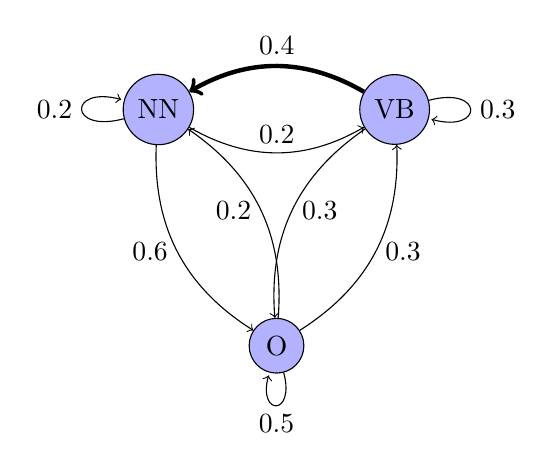
\begin{tikzpicture}
      \node[draw,circle,fill=blue!30] (nn) at (0, 0) {NN};
      \node[draw,circle,fill=blue!30] (vb) at (3, 0) {VB};
      \node[draw,circle,fill=blue!30] (o) at (1.5, -3) {O};
      \draw[->] (nn) edge[loop left] node {0.2} (nn);
      \draw[->] (vb) edge[loop right] node {0.3} (vb);
      \draw[->] (o) edge[loop below] node {0.5} (o);
      \draw[->] (nn) edge[bend right] node[above] {0.2} (vb);
      \draw[->,ultra thick] (vb) edge[bend right] node[above] {0.4} (nn);
      \draw[->] (nn) edge[bend right] node[left] {0.6} (o);
      \draw[->] (o) edge[bend right] node[left] {0.2} (nn);
      \draw[->] (vb) edge[bend right] node[right] {0.3} (o);
      \draw[->] (o) edge[bend right] node[right] {0.3} (vb);
    \end{tikzpicture}
    \caption{In this simple model, we have a state NN for nouns, VB for verbs, and all other states are captured by O. For the example sentence, ``Why not learn ...'', it happens that ``learn'' is a verb, categorized by state \texttt{VB} in our Markov chain depicted above. The probability that the next word is a noun is given by 0.4, denoted by the arrow (transition) from \texttt{VB} to \texttt{NN} (noun).}
  \end{center}
\end{figure}

\paragraph{Transition probability matrix} An equivalent way to represent a Markov chain is through a transition probability matrix $P$, or through what amounts to effectively a simple table. If there are $n$ states in a model, then a transition matrix will be of dimension $n \times n$. Each \emph{row} in the matrix represents transition probabilities from one state to all other states.

\begin{table}[h]
  \begin{center}
    \begin{tabular}{|l | c | c | c|}
      \hline
      & NN & VB & O \\
      \hline
      NN {\color{gray} (noun)} & 0.2 & 0.2 & 0.6 \\
      \hline
      VB {\color{gray} (verb)} & 0.4 & 0.3 & 0.3 \\
      \hline
      O {\color{gray} (other)} & 0.2 & 0.3 & 0.5 \\
      \hline
    \end{tabular}
    \caption{Take a look at the first row: it denotes the transition probabilities \emph{from} state \texttt{NN} i.e. when the current word is a noun. The columns in that row correspond to the future next states, and the entries in the table correspond to the likelihoods of transitioning to the next state given the current state. Notice that the row-sums are unit-valued sicne they are probability distributions.}
  \end{center}
\end{table}

Notice in the table above that it's of dimension $n \times n$. But this means we require a preceding word (and corresponding part of speech tag) in order to predict the next word. Unfortunately, with this set-up we cannot predict the first word in a document, since there is no preceding word! What we can do then is introduce an initial state $\pi$ and include these probabilities in the table in the form of an $(n+1) \times n$ table.

\begin{table}[h]
  \begin{center}
    \begin{tabular}{|l | c | c | c|}
      \hline
      & NN & VB & O \\
      \hline
      $\pi$ {\color{gray} (initial)} & 0.4 & 0.1 & 0.5 \\
      \hline
      NN {\color{gray} (noun)} & 0.2 & 0.2 & 0.6 \\
      \hline
      VB {\color{gray} (verb)} & 0.4 & 0.3 & 0.3 \\
      \hline
      O {\color{gray} (other)} & 0.2 & 0.3 & 0.5 \\
      \hline
    \end{tabular}
    \label{tbl: initialmarkovtable}
    \caption{We encode an initial state such that we can predict the first parts of speech in a document.}
  \end{center}
\end{table}

\vspace{-25pt}
\paragraph{Markov chain recap} A Markov chain consists of a set of $n$ states $Q = \begin{bmatrix} q_1 & q_2 & \ldots & q_n \end{bmatrix}$, and we encode the transition probabilities in a transition matrix $A$
\[
  A = \begin{bmatrix}
    a_{1,1} & \ldots & a_{1,N} \\
    \vdots & \ddots & \vdots \\
    a_{N+1,1} & \ldots & a_{N+1, N}
  \end{bmatrix}
\]

Let's now introduce the hidden Markov model, which are used to decode hidden states of a word; in our context that would be the parts of speech of that word.

\vspace{-10pt}
\subsection{Hidden Markov Model}
The name implies that states are hidden or not directly observable. Going back to the Markov model that has the states for the parts of speech (such as a noun, verb, or other), we can now think of these states as \emph{hidden} because these are not directly observable from our raw text data. This may seem confusing at first: to a human reading the sentence, we can infer what the parts of speech is, e.g. we can clearly tell that ``jump'' is a verb. From a machine's perspective, however, it only sees the text ``jump'' and doesn't know whether it is a verb or a noun. For a machine looking at the text data, it only observes the actual words: these words are observable because they can be seen directly by the machine. The Markov chain model and hidden Markov model have transition probabilities which can be represented by a matrix $A$ of dimension $n+1 \times n$, where $n$ is the number of \emph{hidden} states, e.g. table \ref{tbl: initialmarkovtable}. A hidden Markov model additionally has \emph{emission probabilities}: these describe the transition from the hidden states of our hidden Markov model.

\begin{figure}[h!]
  \begin{center}
    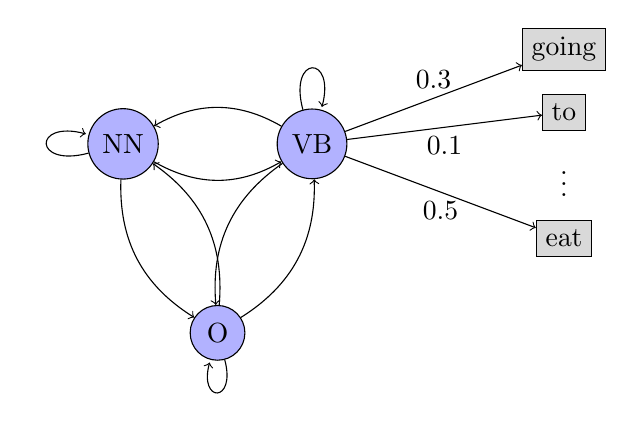
\begin{tikzpicture}[scale=0.8]
      \node[draw,circle,fill=blue!30] (nn) at (0, 0) {NN};
      \node[draw,circle,fill=blue!30] (vb) at (3, 0) {VB};
      \node[draw,circle,fill=blue!30] (o) at (1.5, -3) {O};
      \draw[->] (nn) edge[loop left] node {} (nn);
      \draw[->] (vb) edge[loop above] node {} (vb);
      \draw[->] (o) edge[loop below] node {} (o);
      \draw[->] (nn) edge[bend right] node[above] {} (vb);
      \draw[->] (vb) edge[bend right] node[above] {} (nn);
      \draw[->] (nn) edge[bend right] node[left] {} (o);
      \draw[->] (o) edge[bend right] node[left] {} (nn);
      \draw[->] (vb) edge[bend right] node[right] {} (o);
      \draw[->] (o) edge[bend right] node[right] {} (vb);
      \node[draw,rectangle,fill=gray!30] (going) at (7, 1.5) {going};
      \node[draw,rectangle,fill=gray!30] (to) at (7, 0.5) {to};
      \node (dots) at (7, -0.5) {$\vdots$};
      \node[draw,rectangle,fill=gray!30] (eat) at (7, -1.5) {eat};
      \draw[->] (vb) -- node[above] {0.3} (going);
      \draw[->] (vb) -- node[below] {0.1} (to);
      \draw[->] (vb) -- node[below] {0.5} (eat);
    \end{tikzpicture}
    \caption{\small Here, we describe hidden states with a background shade of \color{blue!80}{blue} \color{black} and observable states with \color{gray!80}{gray}.\color{black} The interpretation here is that if the current parts of speech is a verb, then there is a 50\% chance that the next (observable) word will be ``eat''.}
  \end{center}
\end{figure}

We can of course equivalently represent emission probabilities by a matrix, call it $B$, with dimension $n \times |V|$ where $n$ is the number of states and $|V|$ is the number of observable states.

\begin{table}[h!]
\begin{center}
  \begin{tabular}{| l | l | l | l | l |}
    \hline
    & \textbf{going} & \textbf{to} & \textbf{eat} & $\ldots$ \\
    \hline
    \textbf{NN} {\color{gray!80} noun} & 0.5 & 0.1 & 0.02 & \\
    \textbf{VB} {\color{gray!80} verb} &  0.3 & 0.1 & 0.5 &  \\
    \textbf{O}  {\color{gray!80} other} & 0.3 & 0.5 & 0.068 & \\
    \hline
  \end{tabular}
  \caption{\small In this table, each row is designated for one of the hidden states. A column is designated for each of the observable states. Each row has the property that it's a probability distribution, i.e. $\sum_{j=1}^{|V|} B_{ij} = 1$. You may also at first be surprised that for a fixed observable state (word), it can have strictly positive probabilities for all hidden states (parts of speech); this is actually quite natural because the parts of speech can depend on the context of usage. E.g. in the sentences ``hey lays on his back'' and ``I'll be back'', the word ``back'' has a noun parts of speech in the former sentence and an adverb for the latter.}
\end{center}
\end{table}

\vspace{-20pt}
\paragraph{Calculating probabilities}
Let's learn this first conceptually and then mathematically.

\begin{figure}[h]
  \begin{center}
    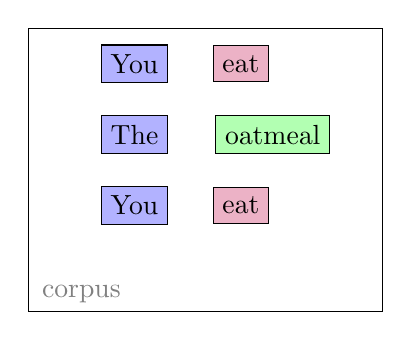
\begin{tikzpicture}[scale=0.9]
      \draw (-0.5, 0) rectangle (4.5, 4);
      \node (corpus) at (0.25, 0.25) {\color{gray} corpus};
      \node[draw,fill=blue!30] at (1, 3.5) {You};
      \node[draw,fill=blue!30] at (1, 2.5) {The};
      \node[draw,fill=blue!30] at (1, 1.5) {You};
      \node[draw,fill=purple!30] at (2.5, 3.5) {eat};
      \node[draw,fill=green!30] at (2.95, 2.5) {oatmeal};
      \node[draw,fill=purple!30] at (2.5, 1.5) {eat};
    \end{tikzpicture}
    \label{fig: trainingcorpuspos}
    \caption{We've depicted a small training corpus; parts of speech tags are denoted by background colors.}
\end{center}  
\end{figure}

To calculate transition probabilities, we'll actually \emph{only} use the parts of speech tags from our training corpus. E.g. to calculate the probabilitiy of a blue speech tag transitioning to a purple one, we first have to count the occurrences of that tag combination in our corpus. In the example depicted above, there are exactly two instances of a blue followed by a purple parts of speech tag. Further, there are exactly three instances of blue parts of speech tags in our entire corpus. So, the conditional probability is $\frac{2}{3}$.

\begin{figure}
  \begin{center}
    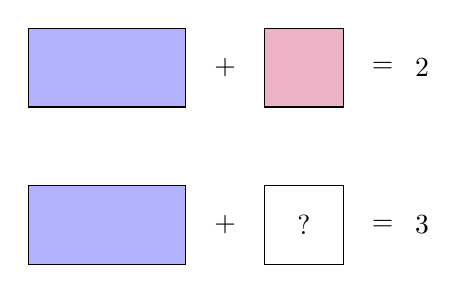
\begin{tikzpicture}
      \draw[fill=blue!30] (0, 0) rectangle (2, 1);
      \node at (2.5, 0.5) {+};
      \draw[fill=purple!30] (3, 0) rectangle (4, 1);
      \draw[fill=blue!30] (0, -2) rectangle (2, -1);
      \node at (2.5, -1.5) {+};
      \draw (3, -2) rectangle (4, -1);
      \node at (3.5, -1.5) {?};
      \node at (4.5, 0.5) {=};
      \node at (5, 0.5) {2};
      \node at (4.5, -1.5) {=};
      \node at (5, -1.5) {3};
    \end{tikzpicture}
    \caption{In our elementary example, we're looking for the conditional probability of transitioning from a blue parts of speech tag to a purple one. There are exactly two of these in the training corpus that appears in figure \ref{fig: trainingcorpuspos}. There are a total of three instances where a blue parts of speech tag appears followed by something else, for our example corpus. Therefore, the transition probability is $\frac{2}{3}$.}
  \end{center}
\end{figure}

To formally calculate transition probabilities, we do so in several steps:
\begin{enumerate}
\item Count occurrences of tag pairs in our training corpus: $C(t_{i-1}, t_i)$.
\item Calculate probabilities using the counts
  \[
    \Pr(t_i | t_{i-1}) = \frac{C(t_{i-1}, t_i)}{\sum_{j=1}^{n} C(t_{i-1}, t_j)},
  \]
  where $n$ is the number of tags in our vocabulary.
\end{enumerate}

As an example, suppose you want to train a model for a Haiku, which is a type of Japanese poetry: your training corpus is the following Haiku from Exra Pound, written in 1913:

\begin{verbatim}
In a station of the Metro
The apparition of these faces in the crowd:
Petals on a wet, black bough.
\end{verbatim}

Consider each line of the corpus as a separate sentence. We'll first add a start token to each line or sentence in order to be able to calculate the initial probabilities using the previously defined formula. We then transform all words in the corpus to lowercase, so that the model is case insensitive.

\paragraph{Populating the transition matrix} Now that we've processed our text corpus, it's time to populate the transition matrix, which will hold the probabilities of going from one state to another in our Markov model. We fill the first column of our matrix with the counts of the associated tags as in figure \ref{fig: countsezra}.

\begin{figure}[h]
  \begin{center}
    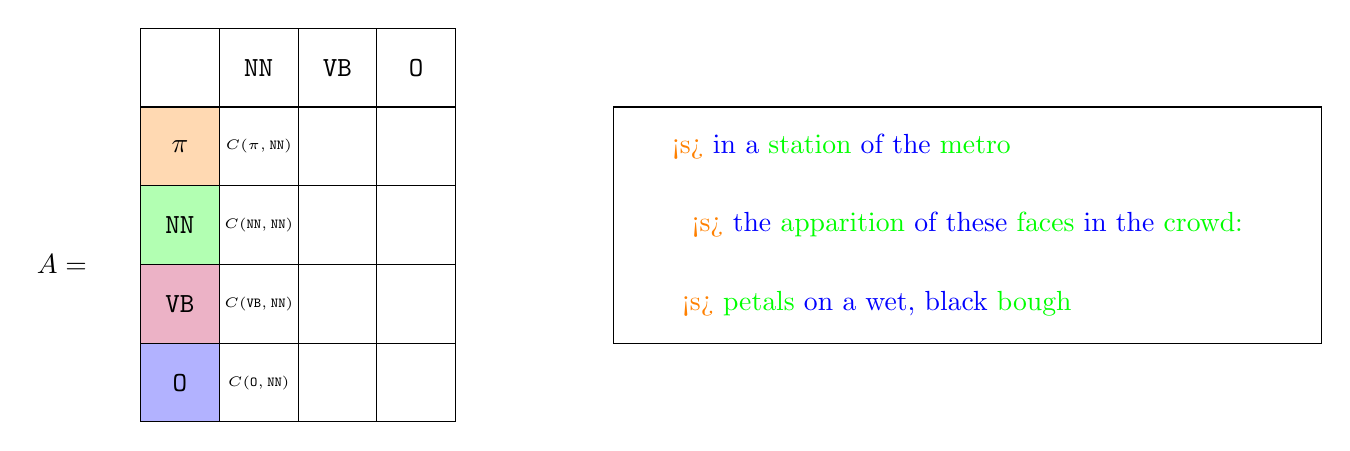
\begin{tikzpicture}
      \node (a) at (-1,2) {$A = $};
      \draw (0, 0) grid (4, 5);
      \draw[fill=orange!30] (0,3) rectangle (1, 4);
      \draw[fill=green!30] (0,2) rectangle (1, 3);
      \draw[fill=purple!30] (0,1) rectangle (1, 2);
      \draw[fill=blue!30] (0,0) rectangle (1, 1);
      % Left column.
      \node at (0.5, 3.5) {$\pi$};
      \node at (0.5, 2.5) {$\texttt{NN}$};
      \node at (0.5, 1.5) {$\texttt{VB}$};
      \node at (0.5, 0.5) {$\texttt{O}$};
      % Top row
      \node at (1.5, 4.5) {$\texttt{NN}$};
      \node at (2.5, 4.5) {$\texttt{VB}$};
      \node at (3.5, 4.5) {$\texttt{O}$};
      % Count formulae
      \node at (1.5, 3.5) {\tiny $C(\pi, \texttt{NN})$};
      \node at (1.5, 2.5) {\tiny $C(\texttt{NN}, \texttt{NN})$};
      \node at (1.5, 1.5) {\tiny $C(\texttt{VB}, \texttt{NN})$};
      \node at (1.5, 0.5) {\tiny $C(\texttt{O}, \texttt{NN})$};
      % Haiku
      \draw (6, 1) rectangle (15, 4);
      \node at (8.9, 3.5) {{\color{orange}<s>} {\color{blue}in a} {\color{green}station} {\color{blue}of the} {\color{green}metro}};
      \node at (10.5, 2.5) {{\color{orange}<s>} \color{blue}{the} \color{green}{apparition} \color{blue}{of these} \color{green}{faces} \color{blue}{in the} \color{green}{crowd}:};
      \node at (9.35, 1.5) {{\color{orange}<s>} \color{green}{petals} \color{blue}{on a wet, black} \color{green}{bough}};
\end{tikzpicture}
  \caption{Using the formula provided and our example corpus, we see that $C(\pi, \texttt{NN}) = 1$, and similarly for our first column 
$C(\texttt{NN}, \texttt{NN}) = 0$
$C(\texttt{VB}, \texttt{NN}) = 0$
$C(\texttt{O}, \texttt{NN}) = 6$. We might further realize that there are no parts of speech that are tagged \texttt{VB}, so this entire row is identically zero. Also, for the last entry in the table given by count $C(\texttt{O}, \texttt{O}) = 8$, realize that we need to count the comma character as its own word-token; we use a sliding window of length two counting bigrams of \texttt{other}-\texttt{other} parts of speech.}
\end{center}
\end{figure}
\label{fig: countsezra}

After having calculated a counts matrix $A$, we cal calculate the transition probabilities according to the formulae $\Pr(t_i, t_{i-1}) = \frac{C(t_{i-1}, t_i)}{\sum_{j=1}^N C(t_{i-1}, t_i)}$: realize that the entries in the table correspond to the numerator term, and the denominator corresponds to row-sums in our table $A$ above.

\begin{table}[h]
  \begin{center}
    \begin{tabular}{|l | c | c | c | c |}
      \hline
      & \texttt{NN} & \texttt{VB} & \texttt{O} & \\
      \hline
      $\pi$ & 1 & 0 & 2 & 3 \\
      \hline
      \texttt{NN} & 0 & 0 & 6 & 6 \\
      \hline
      \texttt{VB} & 0 & 0 & 0 & 0 \\
      \hline
      \texttt{O}  & 6 & 0 & 8 & 14 \\
      \hline
    \end{tabular}
    \caption{In this table, we've simply calculated $C(\cdot, \cdot)$ for each entry given our Haiku by Ezra Pound.}
  \end{center}
\end{table}

E.g. in our example
\[
\Pr(\texttt{NN} | \pi) = \frac{C(\pi, \texttt{NN})}{\sum_{j=1}^N C(\pi, t_j)} = \frac{1}{3}
\]

Or similarly, $\Pr(\texttt{NN} | \texttt{O}) = \frac{C(\texttt{O}, \texttt{NN})}{\sum_{j=1}^N C(\texttt{O}, t_j)} = \frac{6}{14}$. Problems arise: (i) we have an identically zero row which means its conditional probabilities can't be computed, and (ii) a lot of entries in the \emph{counts} matrix $A$ are zero which mean the corresponding transition probabilities are also zero. This won't work if we want our model to generalie well to other haikus, which may contain verbs! To handle this, we can add some small $\epsilon > 0$ to our formula, a technique known as \emph{smoothing}:

\[
  \Pr(t_i | t_{i-1}) = \frac{C(t_{i-1}, t_i) + \epsilon }{\sum_{j=1}^{n} C(t_{i-1}, t_j) + N*\epsilon}.
\]

The consequences of smoothing are (i) we no longer have zeros in our transition probability matrix, and (ii) cases where we had identically zero rows before now have a uniform prior over parts of speech which seems reasonable (e.g. in our example when smoothing is applied $\Pr(\texttt{VB}, \cdot) = \frac{1}{3}$). Note that we may not want to apply smoothing to the first row in our matrix which corresponds to starting from an empty token or start of string: this is because you'll effectively allow strictly positive probabilities for a sentence to start with any word in our vocabulary (including punctuation)!

\paragraph{Populating the emission matrix}  We can now calculate emission probabilities for our hidden Markov model; they are calculated similarly as our transition probabilities.

\begin{figure}[h]
  \begin{center}
    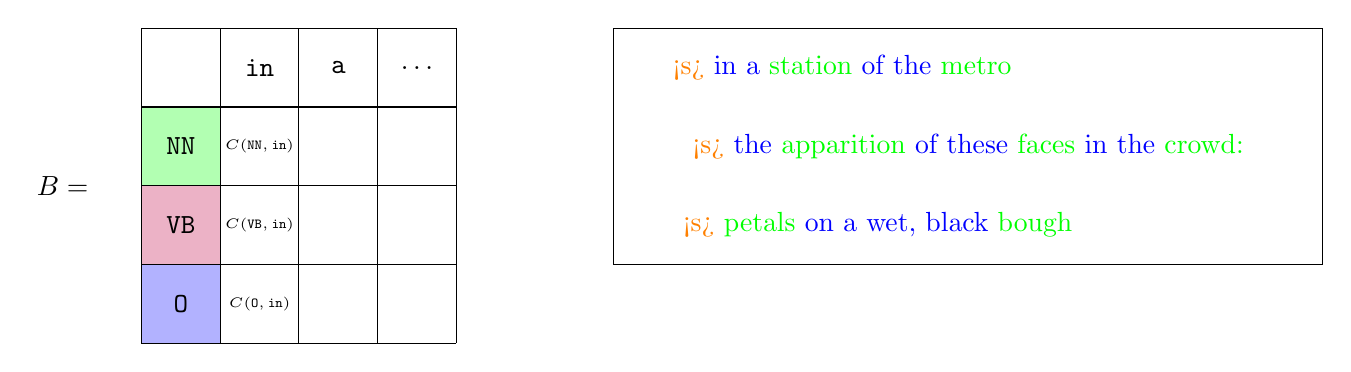
\begin{tikzpicture}
      \node (a) at (-1,2) {$B = $};
      \draw (0, 0) grid (4, 4);
      \draw[fill=green!30] (0,2) rectangle (1, 3);
      \draw[fill=purple!30] (0,1) rectangle (1, 2);
      \draw[fill=blue!30] (0,0) rectangle (1, 1);
      % Left column.
      \node at (0.5, 2.5) {$\texttt{NN}$};
      \node at (0.5, 1.5) {$\texttt{VB}$};
      \node at (0.5, 0.5) {$\texttt{O}$};
      % Top row
      \node at (1.5, 3.5) {$\texttt{in}$};
      \node at (2.5, 3.5) {$\texttt{a}$};
      \node at (3.5, 3.5) {$\ldots$};
      % Count formulae
      \node at (1.5, 2.5) {\tiny $C(\texttt{NN}, \texttt{in})$};
      \node at (1.5, 1.5) {\tiny $C(\texttt{VB}, \texttt{in})$};
      \node at (1.5, 0.5) {\tiny $C(\texttt{O}, \texttt{in})$};
      % Haiku
      \draw (6, 1) rectangle (15, 4);
      \node at (8.9, 3.5) {{\color{orange}<s>} {\color{blue}in a} {\color{green}station} {\color{blue}of the} {\color{green}metro}};
      \node at (10.5, 2.5) {{\color{orange}<s>} \color{blue}{the} \color{green}{apparition} \color{blue}{of these} \color{green}{faces} \color{blue}{in the} \color{green}{crowd}:};
      \node at (9.35, 1.5) {{\color{orange}<s>} \color{green}{petals} \color{blue}{on a wet, black} \color{green}{bough}};
\end{tikzpicture}
  \caption{In this matrix, instead of counting \emph{pairs} of tags, we'll count how often a word is tagged with a specific tag such as \texttt{noun}, \texttt{verb}, or \texttt{other}. For example, in our corpus the \texttt{noun} tag is associated zero times with word ``in'', so $C(\texttt{NN}, \texttt{in}) = 0$. The \texttt{O} tag is associated with the word ``in'' twice, so $C(\texttt{O}, \texttt{in}) = 2$.}
\end{center}
\end{figure}

If we wish to apply smoothing:
\[
  \Pr(w_i | t_i) = \frac{C(t_i, w_i) + \epsilon}{\sum_{j=1}^V C(t_i, w_j) + N * \epsilon} = \frac{C(t_i, w_i) + \epsilon}{C(t_i) + N * \epsilon}
\]
where here $N$ is the number of \emph{tags} and $V$ is the size of our vocabulary.

\subsection{The Viterbi algorithm} So, we've calculated our transition and emission probabilities for the Markov Chain and hidden Markov model. Given the parts of speech tag in these probabilities, you can easily select the most likely next parts of speech tag (or the most probable word). We do so simply looking up the correct entry in the respective row of the transition (or emission) probability matrix. But what if you are given an entire sentence, such as ``why not learn something?'' and you want to compute the most likely parts of speech tags given the sentence and your model. The sequence can be computed using the Viterbi algorithm, which is a graph algorithm. Let's consider a toy model and the example sentence, ``I love to learn''.

\begin{figure}[h!]
  \begin{center}
    \begin{tikzpicture}[scale=0.7]
      % Parts of speech.
      \node[draw,circle,fill=blue!30] (nn) at (-3, 0) {NN};
      \node[draw,circle,fill=blue!30] (vb) at (3, 0) {VB};
      \node[draw,circle,fill=blue!30] (o) at (0, -3) {O};
      \node[draw,circle,fill=blue!30] (pi) at (0, 0) {$\pi$};
      % Emission from verb.
      \node[draw,rectangle,fill=gray!30] (love) at (7, 1.5) {love};
      \node[draw,rectangle,fill=gray!30] (eat) at (7, 0) {eat};
      \node[draw,rectangle,fill=gray!30] (learn) at (7, -1.5) {learn};
      \draw[->] (vb) -- (going);
      \draw[->] (vb) -- (to);
      \draw[->] (vb) -- (eat);
      % Emission from other.
      \node[draw,rectangle,fill=gray!30] (i) at (-2, -5) {i};
      \node[draw,rectangle,fill=gray!30] (to) at (0, -5) {to};
      \node[draw,rectangle,fill=gray!30] (you) at (2, -5) {you};
      \draw[->,orange!80!black,ultra thick] (o) -- node[left] {0.5} (i);
      \draw[->] (o) -- (to);
      \draw[->] (o) -- (you);
      % Emission from noun.
      \node[draw,rectangle,fill=gray!30] (love) at (-5, 1.5) {love};
      \node[draw,rectangle,fill=gray!30] (pony) at (-5, 0) {pony};
      \node[draw,rectangle,fill=gray!30] (sweets) at (-5, -1.5) {sweets};
      \draw[->] (nn) -- (love);
      \draw[->] (nn) -- (pony);
      \draw[->] (nn) -- (sweets);
      % Arrows.
      \draw[->] (pi) -- (nn);
      \draw[->] (pi) -- (vb);
      \draw[->,green!80!black,ultra thick] (pi) -- node[left] {0.3} (o);
      \draw[->] (nn) edge[loop above] node {} (nn);
      \draw[->] (vb) edge[loop above] node {} (vb);
      \draw[->] (o) edge[loop left] node {} (o);
      \draw[->] (nn) edge[bend right] node[above] {} (vb);
      \draw[->] (vb) edge[bend right] node[above] {} (nn);
      \draw[->] (nn) edge[bend right] node[left] {} (o);
      \draw[->] (o) edge[bend right] node[left] {} (nn);
      \draw[->] (vb) edge[bend right] node[right] {} (o);
      \draw[->] (o) edge[bend right] node[right] {} (vb);
    \end{tikzpicture}
    \caption{\small We're given the sequence \texttt{<s> I love to learn}, and we want to find the sequence of hidden states (i.e. parts of speech tags) that have the highest probability for this sequence.}
  \end{center}
\end{figure}

\vspace{-10pt}
\begin{itemize}
  \item Realize that the word ``love'' can be emitted by both noun and verb states. We start from the initial states by selecting the next most probable hidden state which here is the \texttt{O} state as the word ``I'' can't be emitted from any other state in this toy-model. This involves the transition probability shown in {\color{green!80!black}{green}} and the emission probability in {\color{orange!80!black}{orange}}: the joint-probability for observing word ``I'' and with a transition through the \texttt{O} state is 0.15, which we can get by multiplying the two transition and emission probabilities together.
  \item There are then two possibilities or ways to observe the word ``love'' in our model: either by traversing through the hidden states \texttt{NN} or the hidden states \texttt{VB}. Let's suppose that the transition probabilities are the same for going from hidden state \texttt{O} to either of these other two hidden states (e.g. probability is $\frac{1}{2}$); but, perhaps the emission probability for the word ``love'' is higher from hidden state \texttt{VB}, so we choose that path: if the emission probability is also $\frac{1}{2}$ then the joint probability of observing ``love'' with hidden state \texttt{VB} coming from \texttt{O} is $\frac{1}{4}$.
  \item Next, we transition back to hidden state \texttt{O} and emit ``to'' (we must transition back to this hidden state because it is the only one with the emission ``to'') with with combined probability $0.2 \times 0.4 = 0.08$, for example.
  \item Similarly, in the last step we return to the hidden state \texttt{VB} again as there is no other hidden state in the model that can emit observed state ``learn''. 
\end{itemize}

The combined probability of the sentence is the product of individual probabilities that we computed in the steps above. The Viterbi algorithm actually computes several such paths at the same time in order to find the most likely sequence of hidden states. It uses the matrix representation of the hidden Markov model. The algorithm can be split into three main steps: the initialization step, the forward pass, and the backward pass.
Given transition and emission probability matrices, we first populate and use auxiliary matrices $C$ and $D$ where $C$ holds intermediate optimal probabilities and $D$ holds indices of visited states.
As you're traversing the model graph to find the most likely sequence of   parts of speech tags for the given sequence of words $w_1, \ldots, w_k$.
These two matrices $C$ and $D$ are both $n \times k$ where $n$ is the number of parts of speech tags and $k$ is the number of words in the given sequence.

\subsubsection{Initialization} Let's see how to initialize a matrix that will tell you the parts of speech tag of every word. This matrix will tell you the probability that each word belongs to a certain parts of speech. In the initialization step, the first column of each of our matrices $C$ and $D$ are populated. The first column of $C$ represents the probability of the transitions from the start states in the graph to the first tag $t_i$ and word $w_1$.
\begin{figure}[h!]
  \begin{center}
    \begin{tikzpicture}[scale=0.7]
      % Parts of speech.
      \node[draw,circle,fill=blue!30] (nn) at (-3, 0) {$t_2$};
      \node[draw,circle,fill=blue!30] (vb) at (3, 0) {$t_1$};
      \node[draw,circle,fill=blue!30] (o) at (0, -3) {$t_3$};
      \node[draw,circle,fill=blue!30] (pi) at (0, 0) {$\pi$};
      % Emission from verb.
      \node[draw,rectangle,fill=gray!30] (love) at (7, 1.5) {$w_1$};
      \node[draw,rectangle,fill=gray!30] (eat) at (7, 0) {$w_2$};
      \node[draw,rectangle,fill=gray!30] (learn) at (7, -1.5) {$w_3$};
      \draw[->,orange!80!black,ultra thick] (vb) -- (love);
      \draw[->] (vb) -- (to);
      \draw[->] (vb) -- (eat);
      % Emission from other.
      \node[draw,rectangle,fill=gray!30] (i) at (-2, -5) {$w_1$};
      \node[draw,rectangle,fill=gray!30] (to) at (0, -5) {$w_2$};
      \node[draw,rectangle,fill=gray!30] (you) at (2, -5) {$w_3$};
      \draw[->,orange!80!black,ultra thick] (o) -- (i);
      \draw[->] (o) -- (to);
      \draw[->] (o) -- (you);
      % Emission from noun.
      \node[draw,rectangle,fill=gray!30] (love) at (-5, 1.5) {$w_1$};
      \node[draw,rectangle,fill=gray!30] (pony) at (-5, 0) {$w_2$};
      \node[draw,rectangle,fill=gray!30] (sweets) at (-5, -1.5) {$w_3$};
      \draw[->,orange!80!black,ultra thick] (nn) -- (love);
      \draw[->] (nn) -- (pony);
      \draw[->] (nn) -- (sweets);
      % Arrows.
      \draw[->,green!80!black,ultra thick] (pi) -- (nn);
      \draw[->,green!80!black,ultra thick] (pi) -- (vb);
      \draw[->,green!80!black,ultra thick] (pi) -- (o);
      \draw[->] (nn) edge[loop above] node {} (nn);
      \draw[->] (vb) edge[loop above] node {} (vb);
      \draw[->] (o) edge[loop left] node {} (o);
      \draw[->] (nn) edge[bend right] node[above] {} (vb);
      \draw[->] (vb) edge[bend right] node[above] {} (nn);
      \draw[->] (nn) edge[bend right] node[left] {} (o);
      \draw[->] (o) edge[bend right] node[left] {} (nn);
      \draw[->] (vb) edge[bend right] node[right] {} (o);
      \draw[->] (o) edge[bend right] node[right] {} (vb);
      % C-matrix.
      \node (C) at (9, 0) {$C = $};
      \draw (10, -2) grid (15, 2);
      % Top row of C-matrix.
      \node at (11.5, 1.5) {$w_1$};
      \node at (12.5, 1.5) {$w_2$};
      \node at (13.5, 1.5) {$\ldots$};
      \node at (14.5, 1.5) {$w_k$};
      % First column of C-matrix.
      \node at (10.5, 0.5) {$t_1$};
      \node at (10.5,-0.5) {$\vdots$};
      \node at (10.5,-1.5) {$t_N$};
      % Couple of entries in C-matrix.
      \node at (11.5,0.5) {$c_{1,1}$};
      \node at (11.5,-1.5) {$c_{N,1}$};
      % Formula
      \node at (13.8, -3) {$c_{i, 1} = {\color{green!80!black}\pi_i} \times {\color{orange!80!black}b_{i, \texttt{cindex}(w_1)}} = a_{1,i} \times b_{i, \texttt{cindex}(w_1)}$};
    \end{tikzpicture}
    \caption{\small We're considering initialization of $C$'s first column, which describes the transition probability from the start state in the graph to the first tag $t_i$ and word $w_1$. So, it turns out that the first column entries $c_{i, 1}$ are given by the product of the transition probabilities of the initial states with the respective emission probabilities. Since transition probabilities are contained in the first row of our matrix $A$, we can look them up here, and then multiply with the emission probability found in matrix $B$. The function $\texttt{cindex}(\cdot)$ simply returns the column index in the matrix $B$ for the given word fed as input argument.}
  \end{center}
\end{figure}

Above, we considered how to fill in the first column of matrix $C$. What about matrix $D$? Matrix $D$ stores the labels that represents the different states we're traversing when finding the most likely sequence of parts of speech tags for the given sequence of words $w_1, \ldots, w_k$. In the first column, we can simply set all entries to zero, i.e. $d_{i,1} = 0$ for all $i$, as there are no preceeding parts of speech tags we have traversed.

\subsubsection{Forward Pass}
We now use the Viterbi algorithm to continue populating entries in the two matrices we just initialized: $C$ and $D$. We'll see how we can assign parts of speech tags to certain words in the sentence. The remaining entries in $C$ and $D$ are populated column-by-column. For matrix $C$, we have the relation:
\[
  c_{i,j} = \max_k c_{k, j-1} \times a_{k,i} \times b_{i, \texttt{cindex}(w_j)}.
\]

In each $d_{i,j}$, we simply save the corresponding $k$ which maximizes the entry in $C$, i.e.
\[
  d_{i,j} = \argmax_k c_{k, j-1} \times a_{k,i} \times b_{i, \texttt{cindex}(w_j)}.
\]

\subsubsection{Backward Pass} In this section we'll see how we can use the probability matrix, the one we created in the previous section, to create a path, such that we may assign a parts of speech tag to every word. This is the last step of the Viterbi algorithm: retrieving the most likely parts of speech tags for our given sequence of words. Since we've already populated matrices $C$ and $D$, all we have to do is extract the path from the matrix $D$, which represents the sequence of hidden states that most likely generated our sequence of observable words $w_1, \ldots, w_K$. The first step is to calculate the index of the most likely sequence of hidden states generating the given sequence of words, given by
\[
  s = \argmax_i c_{i, K}
\]
where $K$ is the last column in matrix $C$. We use this index to traverse backwards through $D$ to reconstruct the sequence of parts of speech tags.

\paragraph{Example} Suppose we have some input sentence.
\begin{verbatim}
<s> w1 w2 w3 w4 w5
\end{verbatim}
We computed matrix $C$ with the following entries.
\[
  C = \begin{bmatrix}
        & w_1 & w_2 & w_3 & w_4 & w_5 \\
    t_1 & 0.25 & 0.125 & 0.025 & 0.0125 & {\color{green!80!black} 0.01} \\
    t_2 & 0.1 & 0.025 & 0.05 & 0.01 & 0.003 \\
    t_3 & 0.3 & 0.05 & 0.025 & 0.02 & 0.0000 \\
    t_4 & 0.2 & 0.1 & 0.000 & 0.0025 & 0.0003    
  \end{bmatrix}
\]
Then if we inspect the last column for the largest entry, clearly $s = \argmax_i c_{i, K} = 1$, i.e. the highlighted entry in the first row. This index represents the last hidden state you traversed when you observe the word $w_5$: so the most likely hidden state or parts of speech associated with word $w_5$ is $t_1$. 
\[
  D = \begin{bmatrix}
        & w_1 & w_2 & w_3 & w_4 & w_5 \\
    t_1 & 0 & 1 & 3 & 2 & {\color{green!80!black} 3} \\
    t_2 & 0 & 2 & 4 & 1 & 3 \\
    t_3 & 0 & 2 & 4 & 1 & 4 \\
    t_4 & 0 & 4 & 4 & 3 & 1    
  \end{bmatrix}
\]
So, we add $t_1$ to the end of the seqence and look up the next index in $D$, which tells you where you came from.
\begin{verbatim}
<s> w1 w2 w3 w4 w5
                t1
\end{verbatim}
When we examine entry $D_{t_1, w_5}$, we see its value is 3, which indicates that the most likely parts of speech tag for the preceding word $w_4$ is $t_3$.
\begin{verbatim}
<s> w1 w2 w3 w4 w5
             t3 t1
\end{verbatim}
We continue on in this fashion: 
\begin{verbatim}
<s> w1 w2 w3 w4 w5
 pi t2 t3 t1 t3 t1
\end{verbatim}

\paragraph{Implementation note: numerical stability} Multiplying several really small probabilities (or floats) together can result in underflow. To get around this, we use log probabilities, i.e. instead of
\[
  c_{i,j} = \max_k c_{k, j-1} \times a_{k,i} \times b_{i, \texttt{cindex}(w_j)}.
\]
we use
\[
  \log (c_{i,j}) = \max_k \bigg [\log (c_{k, j-1}) + \log (a_{k,i})\bigg ] + \log( b_{i, \texttt{cindex}(w_j)})
\]
where numbers are summed instead of multiplied.

\section{Autocomplete and Language Models}\vspace{.1pt} \hrule height 2pt \smallskip \renewcommand{\arraystretch}{1}% Tighter
\subsection{N-grams}
\paragraph{Overview} Recall that a text corpus is typically a large database of text documents, e.g. all of the pages on Wikipedia, or all of the books from an author, or all tweets from one account. A \emph{language model} is a tool that calculates the probabilities of sentences (which is just a sequence of words). Language models estimate the probability of a subsequent word based on past words. Given the following sentence prefix, how would you fill in the next word?

\begin{verbatim}
Hellow, how are <...>
\end{verbatim}

We'd probably guess ``you''; building an $n$-gram language model can allow us to apply autocomplete to a sentence.

\begin{figure}[h]
  \begin{center}
    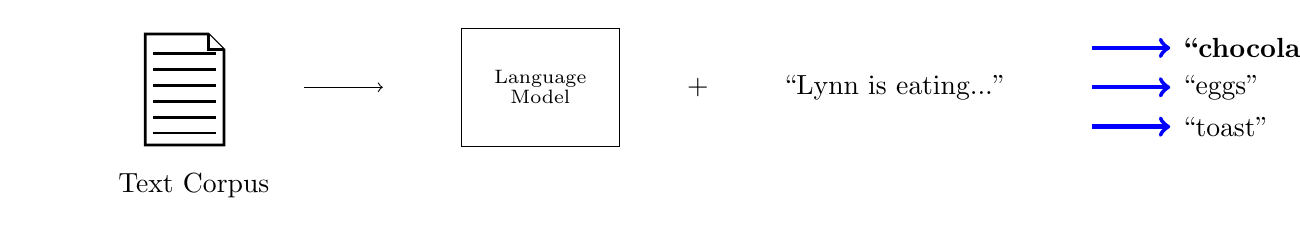
\begin{tikzpicture}
      \foldedpaper{1}
      \node at (-0.4, -0.5) {Text Corpus};
      \draw[->] (1, 0.75) -- (2, 0.75);
      \draw (3, 0) rectangle (5, 1.5);
      \node at (4, 0.75) {$\substack{\textrm{Language} \\ \textrm{Model}}$};
      \node at (6, 0.75) {+};
      \node at (8.5, 0.75) {``Lynn is eating...''};
      \draw[->,ultra thick, blue] (11, 1.25) -- (12, 1.25) node[right,black] {\textbf{``chocolate''}};
      \draw[->,ultra thick, blue] (11, 0.75) -- (12, 0.75) node[right,black] {``eggs''};
      \draw[->,ultra thick, blue] (11, 0.25) -- (12, 0.25) node[right,black] {``toast''};
    \end{tikzpicture}
  \end{center}
\end{figure}

Language models have many applications: e.g. in \emph{speech recognition} to convert the outputs to real words. As a particular example, an acoustic model may convert speech to text and it hears, ``eyes awe of an'', then the speech to text system can use a language model to know that it's more likely the sentence was ``I saw a van''. We can also use language models in \emph{spelling correction}, to identify words that should be replaced based on the sentence they're in; e.g. $\Pr(\textrm{entered the shop to buy}) > \Pr(\textrm{entered the ship to buy})$. Lastly, they can be useful in \emph{augmentative communication}, which are systems that take in a sequence of human hand gestures from a user and help them form words and sentences. E.g. people who are unable to physically talk or sign can instead use simple movements to select words from a menu; then, the system can speak for them, and word prediction using language models can suggest likely words from the menu.

In order to implement sentence autocompletion, we'll take several steps:

\begin{enumerate}
\item Transform your raw text corpus into a language model which returns the   probability of the next word by using the previous words of a sentence.
\item Adapt your language model to deal with words the model hasn't seen before during training; these words are called out of vocabulary words. Here, we apply \emph{smoothing} wherein we assume each out-of-vocabulary word or phrase has been seen at least once in the training corpus.
\item We then can choose the best language model using a perplexity metric.
\end{enumerate}

\paragraph{What is an $N$-gram?} An $N$-gram is simply a \emph{sequence} of words. Note that the order matters, and so it's \emph{not} as simple as a set of words. $N$-grams can also be characters or other elements, but for now let's focus on sequences of words. When we process a corpus, we'll treat punctuation like words, but all other special characters (such as codes), will be removed.
Let's look at an example sentence:
\begin{verbatim}
I am happy because I'm learning
\end{verbatim}
Then, we define \emph{unigrams} for this corpus as the \emph{set} of all unique single words that appear in the text.
\[
  \texttt{Unigrams}: \, \{\color{blue} \textrm{I, am, happy, because, learning} \}
\]
Note that even though the word ``I'' appears in the corpus twice, it's once included once in the \emph{set} of unigrams. \emph{Bigrams} are defined as all sets of two words that appear contiguously (or side by side) in the corpus.
\[
  \texttt{Bigrams}: \, \{\color{blue} \textrm{I am {\color{black},} am happy{\color{black},} happy because{\color{black},} } \color{black} \ldots \}
\]
Notice again that the bigram ``I am'' can be found twice in the text but only is included once in the \emph{set} of bigrams. We emphasize that the words must appear contiguously (or next to each other) in the corpus. As an example, the sequence of words ``I happy'' is not a bigram that appears in the corpus above, and so it has been omitted from the set of bigrams even though each individual word appears in the corpus. We can continue on in this fashion: \emph{trigrams} represent unique \emph{triplets} of words that appear in the sequence together in the corpus.
\[
  \texttt{Trigrams}: \, \{\color{blue} \textrm{I am happy}{\color{black},} \textrm{ am happy because}{\color{black},} \color{black} \ldots \}
\]
Let's define some sequence notation. If we have a corpus of text that consists of 400 words, the sequence of words can be denoted by $w_1, w_2, w_3, \ldots, w_{500}$. The corpus length is denoted by the variable $m$. We will use the notation $w_i^j$ to refer to the sequence of words $w_i, w_{i+1}, \ldots, w_{j-1}, w_j$.

\paragraph{Unigram probability} In our example corpus ``I am happy because I am learning'', the size of the corpus is 7. So, for example, $\Pr(\textrm{I}) = \frac{2}{7}$ since the word ``I'' appears twice in the corpus. Similarly, $\Pr(\textrm{happy}) = \frac{1}{7}$. In general,
\[
  \Pr(w) = \frac{C(w)}{m},
\]
where $C(w)$ denotes the frequency of word $w$ in the corpus.
\paragraph{Bigram probability} In the same example, ``I am happy because I am learning'', what is $\Pr(\textrm{am} | \textrm{I})$? This is given by $\Pr(\textrm{am} | \textrm{I}) = \frac{C(\textrm{I am})}{C(\textrm{I})} = \frac{2}{2} = 1$; i.e. we take the count of the bigrams observed in the corpus divided by the count of the unigram we are conditioning on. In this example, the bigram ``I am'' appears twice, and so does the unigram ``I''; whence we arrive at our calculation. Similarly, $\Pr(\textrm{learning} | \textrm{am}) = \frac{C(\textrm{am learning})}{C(\textrm{am})} = \frac{1}{2}$. The generalized expression is given by:
\[
  \Pr(y|x) = \frac{C(x y)}{\sum_w C(x w)} = \frac{C(x y)}{C(x)},
\]
where we remark that the last equality only follows if $x$ is always followed by some other word!
\paragraph{Trigram probability} Let's consider the same example, ``I am happy because I am learning''. $\Pr(\textrm{happy} | \textrm{I am}) = \frac{C(\textrm{I am happy})}{C(\textrm{I am})} = \frac{1}{2}$. In general,
\[
  \Pr(w_3 | w_1^2) = \frac{C(w_1^2 w_3)}{C(w_1^2)},
\]
where we could re-write the numerator several different ways:
$C(w_1^2 w_3) = C(w_1 w_2 w_3) = C(w_1^3)$.
\paragraph{N-gram probability} Let's generalize further:
\[
  \Pr(w_N | w_1^{N-1}) = \frac{C(w_1^{N-1} w_N)}{C(w_1^{N-1})}
\]
where of course $C(w_1^{N-1} w_N) = C(w_1^N)$.

\paragraph{Modeling the probability of an entire sentence using $N$-grams}
How can we calculate the probability of a sentence, e.g. $\Pr(\textrm{the teacher drinks tea}) = $? Let's recall the definition of conditional probability alongside the chain rule, i.e.
\[
  \Pr(B|A) = \frac{\Pr(A,B)}{\Pr(A)} \implies \Pr(A,B) = \Pr(A) \Pr(B|A).
\]

Generalizing to longer sequences,
\[
  \Pr(A,B,C,D) = \Pr(A) \Pr(B|A) \Pr(C|A,B) \Pr(D | A, B, C).
\]
The product of each successive word is the product of the successive probabilities of all words that came before it in the sequence. We can now apply the chain rule to answering our original question:
\[
\Pr(\textrm{the teacher drinks tea} ) = \Pr(\textrm{the}) \Pr(\textrm{teacher} | \textrm{the}) \Pr(\textrm{drinks} | \textrm{the teacher}) \Pr(\textrm{tea} | \textrm{the teacher drinks}). 
\]

What if the sentence is not in the corpus? The corpus almost never contains the exact sentence we're interested in or even its longer subsequences! E.g.
\[
  \Pr(\textrm{tea} | \textrm{the teacher drinks}) = \underbrace{\frac{C(\textrm{the teacher drinks tea})}{C(\textrm{the teacher drinks})}}_{\textrm{both numerator and denominator terms likely zero}}.
\]

The formula for the probability of the entire sentence can't give a probability estimate in this situation. As the sentence gets longer, the likelihood that more and more words will occur next to each other in this exact order becomes smaller and smaller. E.g. the likelihood that ``the teacher drinks'' appears in the corpus is smaller than the probability of the word ``drinks''.

\paragraph{Applying Markov assumption to model sentences using bigrams} What if instead of looking for all the words before ``tea'', you just consider the previous word which is ``drinks'' in this case, i.e. we assume that
\[
  \Pr(\textrm{tea} | \textrm{the teacher drinks}) \approx \Pr(\textrm{tea} | \textrm{drinks}).
\]
Then, our sentence probability calculate simplifies to
\[
\Pr(\textrm{the teacher drinks tea} ) \approx \Pr(\textrm{the}) \Pr(\textrm{teacher} | \textrm{the}) \Pr(\textrm{drinks} | \textrm{teacher}) \Pr(\textrm{tea} | \textrm{drinks}).
\]
In arguing that the approximation holds, we've effectively argued toward the Markov assumption where the probability of the subsequent word depends \emph{only} on the previous word. Then, what we're saying is that the entire sentence can be modeled using a product of conditional probabilities
\[
  \Pr(w_1^n) \approx \prod_{i=1}^n \Pr(w_i | w_{i-1}).
\]

We could also make this more flexible and instead assert that only the last $N$ words matter, i.e. the Markov assumption here would be that the probability of a word depends only on its recent predecessors up through length $N$. For bigrams, we can approximate the probability
\[
  \Pr(w_n | w_1^{n-1}) \approx \Pr(w_n | w_{n-1})
\]
whereas with $N$-grams we have
\[
  \Pr(w_n | w_1^{n-1}) \approx \Pr(w_n | w_{n-N+1}^{n-1})  .
\]

\paragraph{Starting and ending sentences}
In working with conditional probabilities that operate on a sliding window of two or more words, it's natural to wonder what happens at the beginning or end of a sentence? We'll use two new symbols to denote start and end markers for sentences, and we'll modify our input sentences using these symbols when processing bigrams or $n$-grams.
\begin{itemize}
\item Start of sentence symbol \texttt{<s>}
\item End of sentence symbol \texttt{</s>}
\end{itemize}

Let's revisit our previous sentence, ``the teacher drinks tea''. We've previously asserted that
\[
\Pr(\textrm{the teacher drinks tea} ) \approx \Pr(\textrm{the}) \Pr(\textrm{teacher} | \textrm{the}) \Pr(\textrm{drinks} | \textrm{teacher}) \Pr(\textrm{tea} | \textrm{drinks}).
\]
For the first word ``the'', we don't have context of the previous word, so you can't calculate a bigram probability, which we'll need to make predictions. We'll add in a special term so that each sentence of our corpus can be split into bigrams that we may calculate probabilities for.
\[
\Pr(\textrm{\texttt{<s>} the teacher drinks tea} ) \approx \Pr(\textrm{the} | \texttt{<s>}) \Pr(\textrm{teacher} | \textrm{the}) \Pr(\textrm{drinks} | \textrm{teacher}) \Pr(\textrm{tea} | \textrm{drinks}).
\]
Similar principles apply to $N$-grams. Instead of trying to calculate the sentence probability using a unigram probability for the first word, a bigram probability for the second word, and trigram probabilities for remaining words, as in:
\[
\Pr(\textrm{the teacher drinks tea} ) \approx \Pr(\textrm{the}) \Pr(\textrm{teacher} | \textrm{the}) \Pr(\textrm{drinks} | \textrm{the teacher}) \Pr(\textrm{tea} | \textrm{teacher drinks}).  
\]
We can instead convert our sentence to be ``\texttt{<s><s>} the teacher rinks tea''. So now, the sentence probability becomes the product of trigram probabilities:
\[
  \Pr(w_1^n) \approx \Pr(w_1 | <s> <s>) \Pr(w_2 | <s> w_1) \ldots \Pr(w_n | w_{n-2} w_{n-1}).
\]

For an $N$-gram model, we simply add $N-1$ start tokens \texttt{<s>}. What about end of sentences? Recall that
\[
  \Pr(y|x) = \frac{C(x y)}{\sum_w C(x w)} = \frac{C(x y)}{C(x)}
\]
where in the last step we simplified the denominator in a way that hinges on $x$ always being followed by another word; i.e. when word $x$ is the last word in th sentence, this simplification step does not hold. To see this, suppose we have a Corpus
\begin{verbatim}
Lyn drinks chocolate
John drinks
\end{verbatim}
Then we have a discrepancy in the simplification step above (i.e. it doesn't hold), since clearly
\[
  \sum_w C(\textrm{drinks}\, w) = 1 \neq C(\textrm{drinks}) = 2
\]

To continue using the simplified formula, we need to add end of sentence tokens. But there's another issue at stake: what if we have a very small corpus, e.g.
\begin{verbatim}
<s> yes no
<s> yes yes
<s> no no
\end{verbatim}

There are only two unique words: \{yes, no\}. There are clearly $2^2 = 4$ possible sentences of length two, i.e
\begin{verbatim}
<s> yes yes
<s> yes no
<s> no no
<s> no yes
\end{verbatim}
If we wanted to calculate $\Pr( \texttt{<s>} \, \textrm{yes} \, \textrm{yes})$, we could apply the Markov assumption and work with bigrams to say that it's equal to
\[
\Pr( \texttt{<s>} \, \textrm{yes} \, \textrm{yes}) = \Pr(\textrm{yes} | \texttt{<s>}) \times \Pr(\textrm{yes} | \textrm{yes}) = \frac{C(\texttt{<s>} \, \textrm{yes})}{\sum_w C(\texttt{<s>} \, w)} \times \frac{C(\textrm{yes yes})}{\sum_w C(\textrm{yes} \, w)} = \frac{2}{3} \times \frac{1}{2}.
\]
This is the probability of ``yes yes'' estimated from our corpus.
We can do the same for all of the possible four combinations of bigrams:
\begin{align*}
  \Pr(\texttt{<s>} \textrm{yes} \, \textrm{yes}) = \frac{1}{3}, \hspace{15pt}
  \Pr(\texttt{<s>} \textrm{yes} \, \textrm{no}) = \frac{1}{3}, \hspace{15pt}
  \Pr(\texttt{<s>} \textrm{no} \,\textrm{no} ) = \frac{1}{3}, \hspace{15pt}
  \Pr(\texttt{<s>} \textrm{no} \, \textrm{yes}) = 0
\end{align*}
Notice that $\sum_{2 \textrm{ word}} \Pr(\ldots) = 1$, i.e. we have a probability distribution. We could do the same calculations for all $2^3 = 8$ possible sentences of length three, using the two words in our vocabulary. It turns out that we yield another probability distribution, i.e.
\[
  \Pr(\texttt{<s>} \textrm{yes} \, \textrm{yes} \, \textrm{yes}) = \ldots = \Pr(\texttt{<s>} \textrm{yes} \, \textrm{yes} \, \textrm{no}) = \ldots = \Pr(\texttt{<s>} \textrm{no} \, \textrm{no} \, \textrm{no})
\]
and we again will find that $\sum_{3 \textrm{ word}} \Pr(\ldots) = 1$. But what we really want is for the sum of the probabilities of \emph{all} sentence lengths to be equal to one: in this way we can compare probabilities for sentences of different lengths. In other words, we want
\[
  \sum_{2 \textrm{ word}} \Pr(\ldots) + \sum_{3 \textrm{ word}} \Pr(\ldots) + \ldots = 1
\]

There's a surprisingly simple trick for this: we pre-process our training corpus to simply add in an end of sentence token which we will denote by $</s>$, after each sentence. So sentences get pre-processed:
\begin{verbatim}
the teacher drinks tea => <s> the teacher drinks tea </s>
\end{verbatim}
The probability of our sentence is now modeled by
\[
  \Pr(\textrm{the} | \texttt{<s>}) \Pr(\textrm{teacher} | \textrm{the}) \Pr(\textrm{drinks} | \textrm{teacher}) \Pr(\textrm{tea} | \textrm{drinks}) \Pr(\texttt{<s>} | tea).
\]
This new term captures the probability that our sentence will end after the word ``tea''. This also fixes the issue with probability of the sentences of certain length being equal to one. Does this also resolve our problem with the bigram probability formula?
\begin{verbatim}
<s> Lyn drinks chocolate </s>
<s> John drinks </s>
\end{verbatim}
Now there are two bigrams starting with the word ``drinks'', i.e. $\sum_w C(\textrm{drinks} \, w) = 2$ (which in this example are ``drinks chocolate'' and ``drinks \texttt{</s>}''). Also realize that now this is consistent with $C(\textrm{drinks}) = 2$, so we can continue using our simplified formula for the bigram probability calculation.

What about for $N$-grams in general? It turns out that adding simply one end-of-sentence marker per sentence is enough. To see why, suppose we are processing trigrams and we have the example sentence
\begin{verbatim}
the teacher drinks tea => <s> <s> the teacher drinks tea </s>
\end{verbatim}
We've used two start-of-sentence tokens because we're going to be working with trigrams.

Let's segway and quickly look at a bigram example. Suppose our corpus looks like
\begin{verbatim}
<s> Lyn drinks chocolate </s>
<s> John drinks tea </s>
<s> Lyn eats chocolate </s>
\end{verbatim}
Then from this we can easily calculate conditional probabilities for a sample of bigrams:
\[
  \Pr(\textrm{John} | \texttt{<s>}) = \frac{1}{3}, \hspace{10pt}
  \Pr(\texttt{</s>} | \textrm{tea}) = \frac{1}{1}, \hspace{10pt}
  \Pr(\textrm{chocolate} | \textrm{eats}) = \frac{1}{2}, \hspace{10pt}
  \Pr(\textrm{Lyn} | \texttt{<s>}) = \frac{2}{3}, \hspace{10pt}
\]
Now, let's calculate the probability of the sentence ``Lynn drinks chocolate'', this is given by $\frac{2}{3} \cdot \frac{1}{2} \cdot \frac{1}{2} \cdot \frac{2}{2} = \frac{1}{6} < \frac{1}{3}$, i.e. the probability returned by the model is lower than $\frac{1}{3}$ which is the fraction of sentences which match in the training corpus. This also applies to other sentences in the corpus; this is how the model generalizes!

\subsubsection{The $N$-gram language model}
Here's the general outline:
\begin{itemize}
\item Process the corpus into a Counts matrix; this captures the number of   occurrences of relative $n$-grams.
\item Transform the count matrix into a probability matrix that contains   information about the conditional probability of the $n$-grams.
\item Relate the probability matrix to the language model.
\item Generative language model: we can then use the $n$-gram language model to generate new sentences from scratch.
\end{itemize}

We'll also learn how to deal with technical numerical issues that arise from multiplying a lot of small numbers when calculate the sentence probability.

\paragraph{Counts matrix} Starting with the counts matrix, let's transform into conditional probabilities. The formula for this is given by:
\begin{equation}
  \label{eq: ngramcountstoprobability}
  \Pr(w_n | w_{n-N+1}^{n-1}) = \frac{C(w_{n-N+1}^{n-1}, w_n)}{C(w_{n-N+1}^{n-1})}.
\end{equation}

The numerator of this formula is captured by the Counts matrix for all $n$-grams appearing in the corpus. All unique corpus $(N-1)$-grams make up the rows, and all unique words of the corpus make up the columns.

\begin{table}[h]
  \begin{center}
    \begin{tabular}{|c|c c c c c|}
      \hline
      & \texttt{<s>} & \texttt{</s>} & I & study & learn \\
      \hline
      \texttt{<s>} & 0 & 0 & 1 & 0 & 0 \\
      \texttt{</s>} & 0 & 0 & 0 & 0 & 0 \\
      I & 0 & 0 & 0 & 1 & 1 \\
      study & 0 & 0 & {\cellcolor{orange!80} 1} & 0 & 0 \\
      learn & 0 & 1 & 0 & 0 & 0 \\
      \hline
    \end{tabular}
    \caption{Suppose the corpus is: ``<s> I study I learn </s>''. The rows of       the table above represent the first word of the bigram and the columns represent
      the second word of the bigram. For the bigram ``study I'', it appears once in the corpus. We can calculate hte count matrix in a single pass through the corpus using a sliding window composed of $n=2$ words to represent the bigram: for each bigram you find, increment the value in the count matrix by one.}
  \end{center}
\end{table}

\paragraph{Probability matrix} Now that we've used the counts matrix to provide the numerator for the $n$-gram probability formula, it's time to get the denominator in equation \ref{eq: ngramcountstoprobability}: this is as simple as normalizing each row by its row-sum. I.e.
\[
  \texttt{sum}(\textrm{row}) = \sum_{w \in V} C(w_{n-N+1}^{n-1}, w) = C(w_{n-N+1}^{n-1}).
\]
The row sum is equivalent to the counts of the $(n-1)$-gram prefixes from the formula denominator: this will always be true since the $(n-1)$-gram prefix is always followed by some word. If the prefix was at the end of the sentence, it is now followed by the end of sentence token. Let's create a probability matrix from an example; the corpus is again ``<s> I study I learn </s>''.

\begin{minipage}{0.5\textwidth}
  % \begin{multicols}{2}
    \begin{tabular}{|c|c c c c c|c|}
      \hline
      & \texttt{<s>} & \texttt{</s>} & I & study & learn & sum \\
      \hline
      \texttt{<s>} & 0 & 0 & 1 & 0 & 0 & 1 \\
      \texttt{</s>} & 0 & 0 & 0 & 0 & 0 & 0  \\
      I & 0 & 0 & 0 & 1 & 1 & 2 \\
      study & 0 & 0 &  1 & 0 & 0 & 1 \\
      learn & 0 & 1 & 0 & 0 & 0 & 1 \\
      \hline
    \end{tabular}
  \end{minipage}
  $\overset{\substack{\textrm{Rescale by} \\ \textrm{row sums}}}{\longrightarrow}$
  \begin{minipage}{0.5\textwidth}
    \begin{tabular}{|c|c c c c c|}
      \hline
      & \texttt{<s>} & \texttt{</s>} & I & study & learn \\
      \hline
      \texttt{<s>} & 0 & 0 & 1 & 0 & 0 \\
      \texttt{</s>} & 0 & 0 & 0 & 0 & 0 \\
      I & 0 & 0 & 0 & $\frac{1}{2}$ & $\frac{1}{2}$ \\
      study & 0 & 0 & 1 & 0 & 0 \\
      learn & 0 & 1 & 0 & 0 & 0 \\
      \hline
    \end{tabular}
\end{minipage}

\paragraph{Language model} The next step is to connect the probability matrix with our definition of the language model; the language model is now a simple script that uses the probability matrix to estimate the probability of a given sentence. It estimates the probability by splitting the sentence into $n$-grams and then finding their probability in the probability matrix. Alternatively, the language model can predict the next element of a sequence by extracting the last $(n-1)$-gram from the end of a sequence; after that, the language model finds the corresponding row in the probability matrix and returns the word with highest probability. E.g. let's find the probability of the sentence ``I learn'', using the calculated probabilities from the previous section:
\begin{equation*}
  \Pr(\texttt{<s>} \textrm{ I learn } \texttt{</s>}) = \Pr(\textrm{I} | \texttt{<s>}) \Pr(\textrm{learn} | \textrm{I}) \Pr(\texttt{</s>} | \textrm{learn}) = 1 \times \frac{1}{2} \times 1 = \frac{1}{2}.
\end{equation*}

\paragraph{Log probability} The sentence probability calculation requires multiplication of many small, positive numbers less than unit value:
\[
  \Pr(w_1^n) \approx \prod_{i=1}^{n} \Pr(w_i | w_{i-1}).
\]
This puts us as risk of running into numerical underflow. We use the fact that $\log (ab) = \log a + \log b$ to avoid this problem and proceed by calculating a log probability instead.

\paragraph{Generative language model} One interesting application of a language model is text generation from scratch or using just a small hint. Suppose our corpus is given by:
\begin{verbatim}
<s> Lyn drinks chocolate </s>
<s> John drinks tea </s>
<s> Lyn eats chocolate </s>
\end{verbatim}
E.g. the algorithm might choose ``\texttt{<s>} Lynn'' to start. Next, it will select a bigram that starts with ``Lynn'', perhaps ``Lynn drinks''. Then it chooses a bigram starting with ``drinks'', say ``drinks tea''. Finally, perhaps the model predicts an end of sentence at that point. Notice that our model will always predict end of sentence after predicting ``tea''. How does such an algorithm work?
\begin{itemize}
\item Randomly select among all bigrams starting with the sentence symbol   \texttt{<s>} based on bigram probability; i.e. bigrams with higher values in the probability matrix are more likely to be chosen.
\item Choose a new bigram at random from the bigrams beginning with the   previously chosen word, and add this bigram to your sentence.
\item Continue until the end of sentence token \texttt{</s>} is chosen; this happens when we randomly choose a bigram that starts with the previously chosen word and ends with the token \texttt{</s>}.
\end{itemize}

\subsection{Perplexity} How can you tell how well your language model is performing? Recall that a language model assigns a probability to each sentence, where the model was trained on the corpus. Realize that for sentences appearing in the corpus, the model may assign relatively higher probabilities. Therefore, we should first split the corpus to have some testing and validation data that are \emph{not} used in training. This is similar to other ML workflows: we create training, validation, and test sets of data. The training set is used to train your model, the validation set is used for things like tuning hyper-parameters, and the test set is held out for the end to estimate how the model would perform on unseen data as measured by an accuracy score.

In NLP, there are two main methods for splitting: (i) you can split the corpus by choosing longer continuous segments, such as Wikipedia articles, or (ii) you can randomly choose short sequences of words such as those within the sentences.

\begin{figure}[h]
    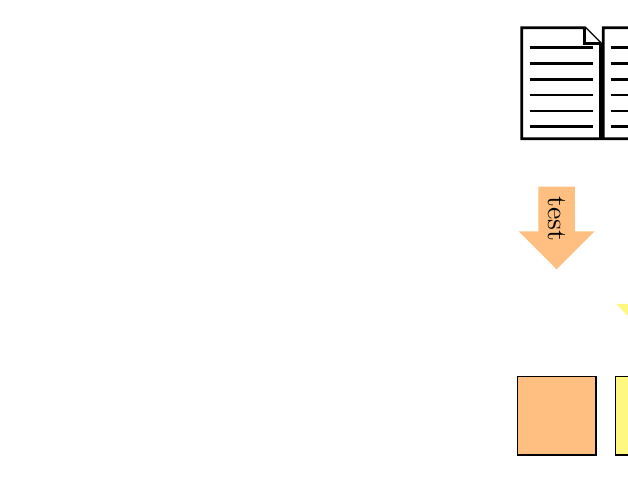
\begin{tikzpicture}[every node/.style={single arrow, draw=none, rotate=270}]
    \foldedpaper{1} \quad \foldedpaper{1}
    \foldedpaper{1} \quad \foldedpaper{1}
    \foldedpaper{1} \quad \foldedpaper{1}
    \node[fill=orange!50] at (-5.75, -1) {test};
    \node[fill=yellow!50] at (-4.5, -1.45) {validation};
    \node[fill=green!50] at (-2, -1) {train};
    \draw[fill=orange!50] (-6.25, -4) rectangle (-5.25, -3);
    \draw[fill=yellow!50] (-5, -4) rectangle (-4, -3);
    \draw[fill=green!50] (-3.75, -4) rectangle (-2.75, -3);
    \draw[fill=green!50] (-2.5, -4) rectangle (-1.5, -3);
    \draw[fill=green!50] (-1.25, -4) rectangle (-0.25, -3);
    \draw[fill=green!50] (0, -4) rectangle (1, -3);
  \end{tikzpicture}
  \caption{Splitting data based on longer continuous sequences such as entire (e.g. Wikipedia) documents: notice that we partition our train, validation, and test sets by document.}
\end{figure}


\begin{figure}[h]
  \begin{center}
  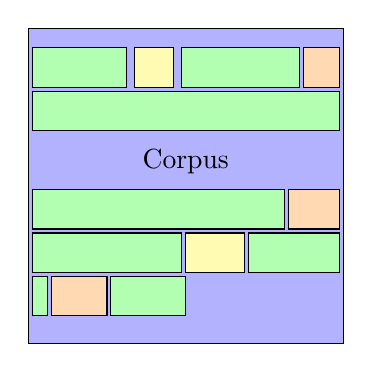
\begin{tikzpicture}
    \draw[fill=blue!30] (-2, -2) rectangle (2, 2);
    % First row.
    \draw[fill=green!30] (-1.95, 1.25) rectangle (-0.75, 1.75);
    \draw[fill=yellow!30] (-0.65, 1.25) rectangle (-0.15, 1.75);
    \draw[fill=green!30] (-0.05, 1.25) rectangle (1.45, 1.75);
    \draw[fill=orange!30] (1.5, 1.25) rectangle (1.95, 1.75);    
    % Second row.
    \draw[fill=green!30] (-1.95, 0.7) rectangle (1.95, 1.2);
    % Corpus label.
    \node at (0, 0.3) {Corpus};
    % Third row of text.
    \draw[fill=green!30] (-1.95, -0.55) rectangle (1.25, -0.05);
    \draw[fill=orange!30] (1.30, -0.55) rectangle (1.95, -0.05);    
    % Fourth row of text.
    \draw[fill=green!30] (-1.95, -1.10) rectangle (-0.05, -0.60);
    \draw[fill=yellow!30] (0, -1.10) rectangle (0.75, -0.60);
    \draw[fill=green!30] (0.80, -1.10) rectangle (1.95, -0.60);
    % Last row of text.
    \draw[fill=green!30] (-1.95, -1.65) rectangle (-1.75, -1.15);
    \draw[fill=orange!30] (-1.70, -1.65) rectangle (-1.00, -1.15);
    \draw[fill=green!30] (-.95, -1.65) rectangle (0, -1.15);
  \end{tikzpicture}
  \end{center}
  \caption{We can also randomly choose short sequences of words such as those that are within sentences to form training, validation, and test sets of data.}
\end{figure}

Once we have our training data split, we can evaluate our model on the test set using the perplexity metric.
\[
  \texttt{PP}(W) = \Pr(s_1, s_2, \ldots, s_m)^{\frac{-1}{m}}.
\]
Where $W$ is the test set containing $m$ sentences $s$, $s_i$ is the $i$-th sentence in the test set (each ending with \texttt{</s>}), $m$ is the number of all words in the entire set including \texttt{</s>} but not including \texttt{<s>}. Perplexity is designed to measure whether a sequence of text looks like it was written by a human as opposed to being generated by a computer program. A text that is written by humans is more likely to have a lower perplexity score, whereas a text chosen at random is more likely to have a higher perplexity score. We start by calculating the probability of all sentences in your test set, and then raise the probability to the power $-1/m$. I.e., perplexity is essentially the inverse probability of the test set normalized by the number of words in the test set. So, the higher the language model estimates the probability of your test set, the lower the perplexity is going to be.\footnote{Perplexity is closely related to entropy, which measures   uncertainty.}

Let's take a look at an example of two language models that are going to return different probabilities for your test set $W$. Suppose there are 100 words in your test set, so $m = 100$. The first model returns a 0.9 probability of the test set, which is very high and indicates the model is effective and is predicting the test set well. The perplexity is near 1: $\Pr(W) = 0.9 \implies \texttt{PP}(W) = 0.9^{\frac{-1}{100}} \approx 1$. The second model has a low probability for the test set, say $10^{-250}$, then $\texttt{PP}(W) = (10^{-250})^{\frac{-1}{100}} \approx 316$ which is very high.

For context, good language models have perplexity scores between $[20, 60]$ and sometiems even lower for English. Perplexities for character level language models (where you track characters instead of words) will be lower.

\paragraph{Perplexity in a bigram language model} In a bigram model, you calculate the products of bigram probabilities for all sentences, then take raise to the power $-1/m$. Realize that the bigger the test set is (i.e. the larger $m$ is), the lower the final perplexity will be. 
\[
  \texttt{PP}(W) = \sqrt[m]{\prod_{i=1}^{m} \prod_{j=1}^{|s_i|} \frac{1}{\Pr(w_j^{(i)} | w_{j-1}^{(i)})}}
\]
where $w_j^{(i)}$ denotes the $j$-th word in the $i$-th sentence.
If all sentences in the test sets are concatanated, the formula can be simplified to the products of probabilities of bigrams in the entire sets.
\[
  \texttt{PP}(W) = \sqrt[m]{\prod_{i=1}^{m} \frac{1}{\Pr(w_i | w_{i-1})}}
\]
where in this context $w_i$ denotes the $i$-th word in the test set.

\paragraph{Log perplexity} Some papers use log-perplexity. This means that we apply the transform
\[
  \texttt{PP}(W) = \sqrt[m]{\prod_{i=1}^{m} \frac{1}{\Pr(w_i | w_{i-1})}} \longrightarrow \log \texttt{PP}(W) = \frac{-1}{m} \sum_{i=1}^{m} \log_2 \Pr(w_i | w_{i-1}).  
\]
In a good model with perplexity between $[20,60]$, the log-perplexity would range from $[4.3, 5.9]$.

\subsection{Unknown Words}
Sometimes, we'll encounter words that we did not see during training, i.e. unknown or \emph{out-of-vocabulary} words; we can add a special new word \texttt{UNK} to our probability calculations from our training corpus to accommodate this. We can also consider which words should be considered known by our vocabulary. Let's look at this in further detail.

\paragraph{What is an out of vocabulary word?} A vocabulary is a set of unique words supported by a language model. There are certain tasks such as question answering where you will encounter and generate only words from a fixed set of words: i.e. a chatbot can only answer limited sets of questions. The fixed set of words is what's formally called a \emph{closed vocabulary}. But in other use cases, you have to deal with words you haven't seen before which results in what's called an \emph{open vocabulary}. E.g. you might see a name of a new city in your training data. The unknown words are called out of vocabulary words (or OOV for short).

\paragraph{Adding a new special word \texttt{UNK}} One way to deal with the unknown words is to replace them by a special word \texttt{<UNK>}. This literally means replacing each instance of an unknown word with \texttt{<UNK>} in your data.
\begin{enumerate}
\item Create a vocabulary $V$.
\item Replace any word that is in the training corpus but \emph{not} in     vocabulary by \texttt{<UNK>}.
\item Count the probabilities with \texttt{<UNK>} as with any other word.
\item Now, we may apply the $n$-gram language model probability calculations in the same way as before, just with the addition of \texttt{<UNK>}.
\end{enumerate}
E.g. suppose we've been given the following training corpus:
\begin{verbatim}
<s> Lyn drinks chocolate </s>
<s> John drinks tea </s>
<s> Lyn eats chocolate </s>
\end{verbatim}
We have decided to only include words in our vocabulary that appear at least twice in our training corpus. The post-processed corpus will then look like
\begin{verbatim}
<s> Lyn drinks chocolate </s>
<s> <UNK> drinks <UNK> </s>
<s> Lyn <UNK> chocolate </s>
\end{verbatim}
Our vocabular includes words with frequency (in our training corpus) greater than or equal to two, i.e. $V = \{\textrm{Lyn, drinks, chocolate}\}$.
If we were given a new sentence, say ``Adam drinks chocolate'', then we would also replace any out-of-vocabulary words with \texttt{<UNK>}, i.e.
\begin{verbatim}
<s> Adam drinks chocolate </s>  -->  <s> <UNK> drinks chocolate </s>
\end{verbatim}

\paragraph{How to create a vocabulary $V$} We can create a vocabulary from a training corpus based on different criteria.

\begin{itemize}
\item Minimum word frequency $f$ (usually a small number): i.e. only include words in the vocabulary $V$ that appear at least $f$ times in our training corpus. Replace all words that appear fewer than $f$ times with \texttt{<UNK>}. This ensures that the words that ``we care about a lot'', i.e. the ones which repeat a lot in our training corpus, are certainly present in our vocabulary.
\item Alternatively, we could decide what the maximum size of our vocabulary should be, i.e. fix $|V|$, and then include words with highest frequency until we fill the vocabulary.
\end{itemize}

\paragraph{Effect of \texttt{<UNK>} on perplexity?} One thing to be mindful of when using \texttt{<UNK>}s is the effect on measures of perplexity. It turns out that the more \texttt{<UNK>}s we use, the lower the perplexity tends to be; it'll look like our language model is getting better and better, but our model might be prone to spitting out a sequence of \texttt{<UNK>}s with high probability instead of a meaningful sentence. Due to this limitation, we recommend using \texttt{<UNK>}s sparingly. Lastly, and for the aforementioned reasons, it's important to only compare models using perplexity when they have the same vocabulary $V$.

\subsection{Rare Words and \emph{Smoothing}} When we train an $n$-gram model on a limited corpus, some of the probabilities for rare words may be skewed; we can remedy this using a technique known as \emph{smoothing}. We'll first see an example of how an $n$-gram missing from the corpus can affect the estimation of the $n$-gram probability. Then, we'll cover popular smoothing techniques. And finally, we'll touch on other methods such backoff and interpolation.

\paragraph{Missing $n$-grams} We have resolved the issue of completely unknown words. But there is still missing information from our language model: i.e. how can we manage the probability of an $n$-gram made up of words appearing in the corpus, but where the $n$-gram itself is not present? Recall our example corpus:
\begin{verbatim}
<s> Lyn drinks chocolate </s>
<s> John drinks tea </s>
<s> Lyn eats chocolate </s>
\end{verbatim}
Notice that each of the words $\{\textrm{John, eats}\}$ are present in the corpus, but that the bigram ``John eats'' is not. The count of the bigram ``John eats'' is zero, and correspondingly the probability returned by a naive model would be zero as well. I.e. the numerator and denominator terms on the right hand side of the following expression
\[
  \Pr(w_n | w_{n-N+1}^{n-1}) = \frac{C(w_{n-N+1}^{n-1}, w_n)}{C(w_{n-N+1}^{n-1})}
\]
can be zero; everything that doesn't occur in the training corpus is considered impossible.
\subsubsection{Techniques for Smoothing} This is a technique that can help with the aforementioned problem of missing $n$-grams when constructing $n$-gram language models. Recall that we've used smoothing in constructing the transition probabilities for parts of speech tagging. We'll use the same idea for $n$-gram probabilities.

\paragraph{Add one smoothing}
Let's focus on a technique known as ``add-one smoothing'' otherwise known as \emph{Laplacian smoothing}, which mathematically changes our probability calculations to
\[
  \Pr(w_n | w_{n-N+1}^{n-1}) = \frac{C(w_{n-1}, w_n) + 1}{\sum_{w \in V} \left[C(w_{n-1}, w) + 1\right]} = \frac{C(w_{n-1}, w_n) + 1}{C(w_{n-1}) + |V|}.
\]
This change can be interpreted as simply adding one occurrence to each bigram; this means that bigrams that were missing from the corpus will now have a strictly nonzero probability. In the denominator, we are adding one for each possible bigram, starting with the word $w_{n-1}$: this corresponds to adding one to each cell in the row indexed by the word $w_{n-1}$ in the counts matrix. We repeat this for as many times as there are words in the vocabulary. Because the one in the sum doesn't depend on index $w$, we can take it out of the sum and replace with $|V|$. This technique really \emph{only works} when the real counts are large enough to outweigh the ``plus one'' term however: otherwise, the probabilities of missing words would be too high. That said, add-one-smoothing helps quite a lot because now there are no bigrams with identically probability.

\paragraph{Add $k$ smoothing} If you have a larger corpus, you can instead add $k > 1$. This technique makes the probabilities \emph{even smoother}. The formula is similar:
\[
  \Pr(w_n | w_{n-N+1}^{n-1}) = \frac{C(w_{n-1}, w_n) + k}{\sum_{w \in V} \left[C(w_{n-1}, w) + k\right]} = \frac{C(w_{n-1}, w_n) + k}{C(w_{n-1}) + k \times |V|}.
\]
Other more advanced smoothing methods include \href{https://en.wikipedia.org/wiki/Kneser%E2%80%93Ney_smoothing}{Kneser-Ney} or   \href{https://en.wikipedia.org/wiki/Good%E2%80%93Turing_frequency_estimation}{Good-Turing}.

\paragraph{Backoff} There's another technique to dealing with $n$-grams that do not occur in the training corpus, and that is to use information about $(n-1)$-grams, $(n-2)$-grams, and so on. With the backoff approach, if $n$-gram information is missing, you use $(n-1)$-gram, but if that's also missing you resort to using $(n-2)$-gram, and so on until you find a non-zero probability. Using the lower level $n$-grams, i.e. $(n-1)$-gram, $(n-2)$-gram, all the way down to a unigram, distorts the probability distribution. Especially for smaller corpora, some probability needs to be discounted from the higher level $n$-gram in order to use it for lower-level $n$-grams. \href{https://en.wikipedia.org/wiki/Katz%27s_back-off_model}{Katz backoff} method uses this technique when counting. For large sized, web-scale corpora, a method known as \href{https://www.aclweb.org/anthology/D07-1090.pdf}{``stupid-backoff''} has also been shown to be effective: in this approach, no discounting is applied. If a higher order $n$-gram probability is missing, lower order $n$-grams are used, just multiplied by some constant (a constant of about $\frac{4}{10}$ was shown to work well empirically). Let's apply Backoff to an example
\begin{verbatim}
<s> Lyn drinks chocolate </s>
<s> John drinks tea </s>
<s> Lyn eats chocolate </s>
\end{verbatim}
In this example, the probability of the trigram ``John drinks chocolate'' can't be directly estimated from the corpus. So, the probability of the bigram ``drinks chocolate'', multiplied by some constant (say $c = \frac{4}{10}$), would be used instead.
\[
  \Pr(\textrm{chocolate} | \textrm{John drinks}) \approx c \times \Pr(\textrm{chocolate} | \textrm{drinks}).
\]
\paragraph{Interpolation} Another alternative to backoff is to use a linear interpolation of all orders of $n$-gram. This means that you would always combine the weighted probability of the $n$-gram, $(n-1)$-gram, all the way down to unigrams. E.g. when calculating the probability of the trigram
\[
\Pr(\textrm{chocolate} | \textrm{John drinks}) = \lambda_1 \Pr(\textrm{chocolate} | \textrm{John drinks}) + \lambda_2 \Pr(\textrm{chocolate} | \textrm{drinks}) + \lambda_3 \Pr(\textrm{chocolate}),
\]
where $\lambda_1 > \lambda_2 > \lambda_3$ and $\sum_i \lambda_i = 1$. More generally,
\[
  \hat \Pr(w_n | w_{n-2} \, w_{n-1}) = \lambda_1 \Pr(w_n | w_{n-2} \, w_{n-1}) + \lambda_2 \Pr(w_{n} | w_{n-1}) + \lambda_3 \Pr(w_n) \hspace{25pt} \textrm{ where} \hspace{25pt} \sum_i \lambda_i = 1.
\]
The lambdas are \emph{learned} from the validation parts of the corpus: you get them by maximizing the probability of sentences in the validation set. To do this, you use a fixed language model trained from the training parts of the corpus to calculate $n$-gram probabilities and then optimize the $\lambda$s. The interpolation can be apply to general $n$-grams by applying more $\lambda$s.

\section{Word Embeddings with Neural Networks}\vspace{.1pt} \hrule height 2pt \smallskip \renewcommand{\arraystretch}{1}% Tighter
Word vectors, also known as word embeddings, are the cornerstone of NLP. Recall that we've previously used word embeddings to find semantic analogies between words, and also to calculate distances between words and similarities between words.
Separately, it's possible to perform sentiment analysis by combining word embeddings with a classifier, or to classify customer reviews (or comments) from user feedback surveys. Advanced uses of word embeddings include machine translation systems, information extraction, and question-answering.
Our key learning objectives in this section are:

\begin{figure}[h]
  \begin{center}
    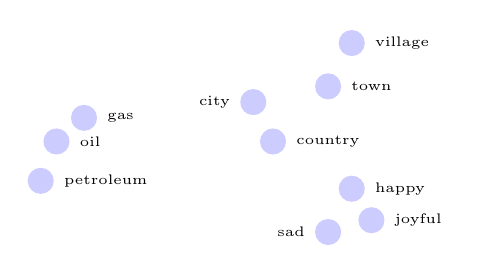
\begin{tikzpicture}[
      mycirc/.style={circle,fill=blue!20, minimum size=0.2cm}
    ]
    % Oil related
    \node[mycirc,label=right:{\tiny petroleum}] at (-0.95, -0.5) {};
    \node[mycirc,label=right:{\tiny oil}] at (-0.75, 0) {};
    \node[mycirc,label=right:{\tiny gas}] at (-0.4, 0.3) {};
    % Geographies
    \node[mycirc,label=left:{\tiny city}] at (1.75, 0.5) {};
    \node[mycirc,label=right:{\tiny country}] at (2, -0) {};
    \node[mycirc,label=right:{\tiny town}] at (2.7, 0.7) {};
    \node[mycirc,label=right:{\tiny village}] at (3, 1.25) {};
    % % Emotions
    \node[mycirc,label=right:{\tiny happy}] at (3, -0.6) {};
    \node[mycirc,label=right:{\tiny joyful}] at (3.25, -1) {};
    \node[mycirc,label=left:{\tiny sad}] at (2.7, -1.15) {};
  \end{tikzpicture}
  \caption{As an example, word embeddings help capture semantic relationships. When we project the word embeddings into a lower dimensional space, we can often times see clusters of words that represent related concepts.} 
  \end{center}
\end{figure}

\begin{itemize}
  \item Identify the key concepts of word representations: we will represent     words numerically such that we may use them in mathematical models.
\item Generate word embeddings: we'll see how we can \emph{learn} word   embeddings from data with some commonly used methods.
\item Prepare text for machine learning: transform a corpus of text into   training sets for a machine learning model.
\item Implement the continuous bag-of-words model, which is one of the many ways word embedding can be created.
\end{itemize}

\subsection{Word Representations} Let's now learn how to create a matrix to represent all of the words in our vocabulary. Each vector in the matrix will correspond to one of the words.

\paragraph{Naively: represent words as integers}
The simplest way to represent words as numbers is, for a given vocabulary, to assign a unique integer ID to each word.
\begin{table}[h]
  \begin{center}
    \begin{tabular}{c c}
      \hline
      Word & Number \\
      \hline
      a & 1 \\
      able & 2 \\
      about & 3 \\
      $\ldots$ & $\ldots$ \\
      hand & 615 \\
      $\ldots$ & $\ldots$ \\      
      happy & 621 \\
      $\ldots$ & $\ldots$ \\
      zebra & 1000 \\
      \hline
    \end{tabular}
  \end{center}
\end{table}
E.g. based on a vocabulary of 1,000 basic English words, we might assign the number one to word ``a'', the number two to ``able'', and so on until we assign something like one-thousand to ``zebra''. While this schema might seem simple, the problem is that the order of words, alphabetical in this example, doesn't make much sense from a semantic perspective. For example, there's really no good intuitive reason why ``happy'' should be assigned a greater number than ``hand'' for instance, or a smaller one than ``zebra''.

\paragraph{One-hot vectors}
\label{par: onehotvectors}
Instead, let's try using a numerical column vector to represent a word of the vocabulary. If again we have a vocabulary of 1,000 words, each vector would contain 1,000 elements and each row would be labeled with one of the words. We can now use a one-hot encoding: place a one in the row that has the same label and a zero everywhere else. For example, the word ``happy'' would be represented as a column vector where there is a unit-value in the row corresponding to ``happy'' and zeros for all other rows in the vocabulary.

\begin{table}[h]
  \begin{center}
    \begin{tabular}{c l}
      ``happy'' & \\
      0 & a \\
      0 & able \\
      0 & about \\
      $\vdots$ & $\vdots$ \\
      0 & hand \\
      $\vdots$ & $\vdots$ \\      
      1 & happy \\
      $\vdots$ & $\vdots$ \\
      0 & zebra \\
    \end{tabular}
    \caption{The above column-vector is a one-hot representation of the word ``happy''. It has as many row-entries as there are elements in our vocabulary.}
  \end{center}
\end{table}

\paragraph{Pros and cons of one-hot vectors}
Note that one-hot vectors have the advantage over using integers beacuse one-hot vectors do not imply any relationship between two words (other than they are either equal or not), e.g. each vector simply says the word is either ``happy'' or it's not, or the word is either ``zebra'' or it's not. There are, however, two major limitations for using one-hot vectors in NLP: (i) barring the smallest of vocabularies, these word vectors are going to be huge, which means processing/working with them on a compute will take lots of space and time, and (ii) their representation again doesn't carry the words semantic meaning. For instance, \emph{all} words that are not the same have the same distance between them, e.g. the word ``happy'' is just as similar to the word ``paper'' as it is to the word ``excited'' (but intuitively, we would think that ``happy'' and ``excited'' are closer in distance, of course).

\paragraph{Mapping between integer representation to one-hot vectors} Realize that we can easily map back and forth between one-hot vectors and the integer representation for a word. We do this simply by mapping the words in the rows to their corresponding row number. In this way, e.g. ``happy'' may be word 621 would be represented as a column vector with a 1 in row 621, and it can also be represented as the integer-ID 621.

\subsection{Word Embeddings} Although there are basic ways to represent words as numbers, these representations fail to carry meaning. Let's now move to embeddings, which are vectors that do indeed carry meaning.

\paragraph{Intuition for how a (scalar) vector representation can capture semantic meaning}
Let's first get an intuition for how word vectors can carry the meaning of words, starting in 1D.

\begin{figure}[h]
  \begin{center}
    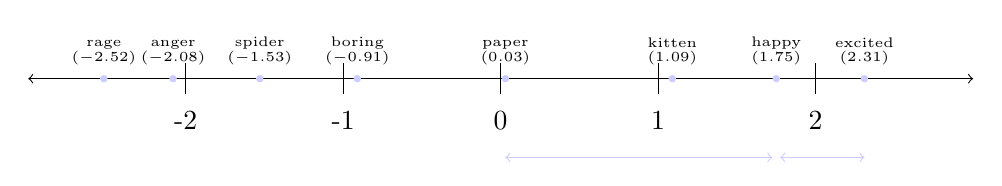
\begin{tikzpicture}[scale=2,
      mycirc/.style={circle,fill=blue!20, scale=0.1mm}
    ]
    \draw[<->] (-3, 0) -- (3, 0);
    \foreach \x in {-2, -1, 0, 1, 2} {
      \draw (\x, -0.1) -- (\x, 0.1) node[below=0.5cm] {\x};
    }
    \node[mycirc,label=above:{\tiny {$\substack{\textrm{rage} \\ (-2.52)}$}}] at (-2.52, 0) {};
    \node[mycirc,label=above:{\tiny {$\substack{\textrm{anger} \\ (-2.08)}$}}] at (-2.08, 0) {};
    \node[mycirc,label=above:{\tiny {$\substack{\textrm{spider} \\ (-1.53)}$}}] at (-1.53, 0) {};
    \node[mycirc,label=above:{\tiny {$\substack{\textrm{boring} \\ (-0.91)}$}}] at (-0.91, 0) {};
    \node[mycirc,label=above:{\tiny {$\substack{\textrm{paper} \\ (0.03)}$}}] at (0.03, 0) {};
    \node[mycirc,label=above:{\tiny {$\substack{\textrm{kitten} \\ (1.09)}$}}] at (1.09, 0) {};
    \node[mycirc,label=above:{\tiny {$\substack{\textrm{happy} \\ (1.75)}$}}] at (1.75, 0) {};
    \node[mycirc,label=above:{\tiny {$\substack{\textrm{excited} \\ (2.31)}$}}]     at (2.31, 0) {};
    \draw[<->,color=blue!20] (0.03, -0.5) -- (1.725, -0.5);
    \draw[<->,color=blue!20] (1.775, -0.5) -- (2.31, -0.5);
\end{tikzpicture}
\caption{Consider a horizontal number line, where words to the left of the origin are considered negative in some way and words on the right are considered positive in some way. Words that are much more negative are further to the left, and words that are much more positive are further to the right. You could store their positions as scalars (or vectors of length 1). Notice that you can use any decimal value instead of binary values $\{0, 1\}$, which means that we can now say that ``happy'' and ``excited'' are more similar to each other compared with the word ``paper'': their distance is smaller.}
\end{center}
\end{figure}

\paragraph{Extending our intution to more than 1 dimension}
Let's now consider how adding a second dimension can help capture more meaning of words.

\begin{figure}[h!]
  \begin{center}
    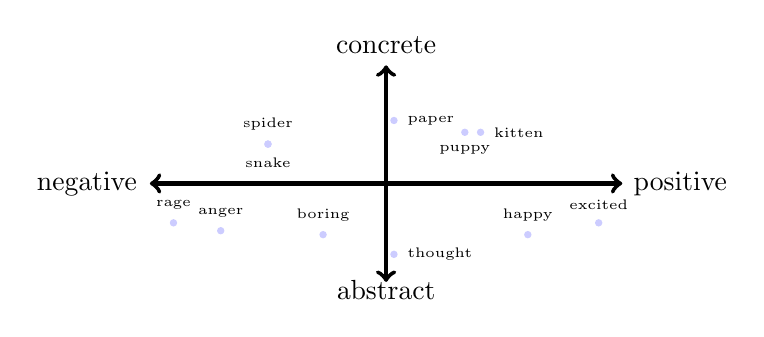
\begin{tikzpicture}[
      mycirc/.style={circle,fill=blue!20, scale=0.1mm}
    ]
    \draw[<->,ultra thick] (-3,0)--(3,0) node[right]{positive};
    \node at (-3.8, 0) {negative};
    \draw[<->,ultra thick] (0,-1.25)--(0,1.5) node[above]{concrete};
    \node at (0, -1.35) {abstract};
    \node[mycirc,label=above:{\tiny spider}] at (-1.5, 0.5) {};
    \node[mycirc,label=below:{\tiny snake}] at (-1.5, 0.5) {};
    % lower left quadrant.
    \node[mycirc,label=above:{\tiny rage}] at (-2.7, -0.5) {};
    \node[mycirc,label=above:{\tiny anger}] at (-2.1, -0.6) {};
    \node[mycirc,label=above:{\tiny boring}] at (-0.8, -0.65) {};
    % lower right quadrant.
    \node[mycirc,label=right:{\tiny thought}] at (0.1, -0.9) {};
    \node[mycirc,label=above:{\tiny happy}] at (1.8, -0.65) {};
    \node[mycirc,label=above:{\tiny excited}] at (2.7, -0.5) {};
    % upper right quadrant.
    \node[mycirc,label=right:{\tiny paper}] at (0.1, 0.8) {};
    \node[mycirc,label=below:{\tiny puppy}] at (1, 0.65) {};
    \node[mycirc,label=right:{\tiny kitten}] at (1.2, 0.65) {};    
  \end{tikzpicture}
  \caption{We have now extended our word representation into two dimensions: the vertical number line represents how concrete (or abstract) the object is; words that are higher on the number line are more concrete and words that are lower on the number line are more abstract. Notice that words that are both more concrete and positve like ``puppy'' and ``kitten'' are close together. We can store the two numbers that represent the position on the cartesian plane as a vector of length two. So, what we've done here is to represent the vocabulary of words with a small vector of length two. We've gained a little bit of meaning while also giving up some precision: the vector is less precise than one-hot vectors in that it's possible for two words to be located on the same point in this 2D plot, such as the words ``snake'' and ``spider''.}
\end{center}
\end{figure}

Word embeddings represent words in a vector form that both has relatively low dimension (e.g. hundreds to thousands), which makes it practical for calculations, and carries the semantic meaning between words, which makes it possible to determine how semantically close a pair of words really are. In a general purpose vocabulary, we might expect the vector representation for ``forest'' to be similar to ``tree'', but for both of those to be very different for the vector ``tickets''. Using word vectors, we can also fill in analogies: e.g. ``Paris is to France as Rome is to?''. Encoding the meaning of words is also the first step toward encoding the meaning of entire sentences, and this is the foundation for more complex NLP use cases (such as question-answering and translation).

\subsubsection{How to Create Word Embeddings} To create word embeddings we need two things: a corpus of text and an embedding method.

\paragraph{Choice of corpus}
The corpus contains the words you want to embed organized in the same way they would be used in the context of interest. For example, if you want to generate embeddings based on Shakespeare, then your corpus would be the full and original text of Shakespeare
and \emph{not} study notes, slide presentations, or keywords from Shakespeare, for example. The context of a word refers towards other words or a combination of other words said to occur around that particular word; the context is important as this is what will give meaning to  each word embedding. I.e. a simple vocabulary list of Shakespeare's most common words would \emph{not} be enough to create an embedding. A corpus could be either a general purpose set of documents such as Wikipedia articles, \emph{or} it could be more specialized such as an industry or enterprise specific corpuse to capture the nuances of the context (e.g. for NLP use cases on legal topics, you could use contracts and law books as the corpus).

\begin{figure}[h]
  \begin{center}
    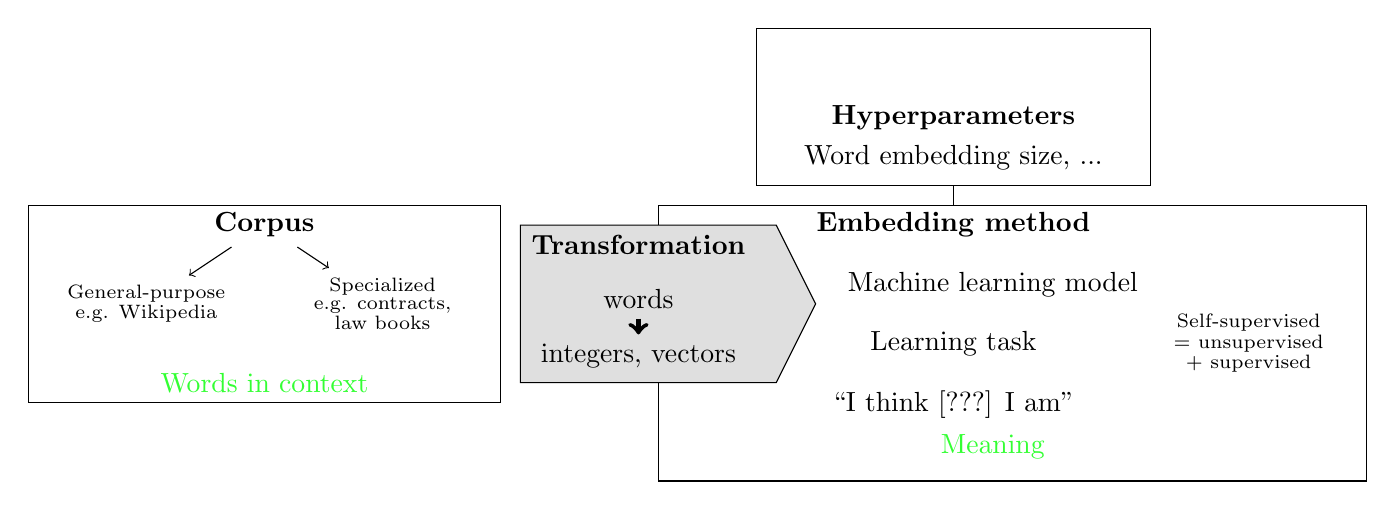
\begin{tikzpicture}
      % Corpus.
      \node (corpus) at (-3, 1) {\textbf{Corpus}};
      \node (general) at (-4.5, 0) {$\substack{\textrm{General-purpose} \\           \textrm{e.g. Wikipedia}}$};
      \node (specialized) at (-1.5, 0) {$\substack{\textrm{Specialized} \\                               \textrm{e.g. contracts,} \\ \textrm{law books}}$};
\draw[->] (corpus) -- (general);
\draw[->] (corpus) -- (specialized);
      \node (context) at (-3, -1) {\color{green!80} Words in context};
      \draw (-6, -1.25) rectangle (0, 1.25);
% Embedding method.
\node (embeddingmethod) at (5.75, 1) {\textbf{Embedding method}};
\node (mlmodel) at (6.25, 0.25) {Machine learning model};
\node (learningtask) at (5.75, -0.5) {Learning task};
\node (selfsupervised) at (9.5, -0.5) {$\substack{\textrm{Self-supervised} \\ =     \textrm{ unsupervised} \\ + \textrm{ supervised}}$};
\node[below=2mm of learningtask] {``I think [???] I am''};
\node[below=15mm of mlmodel] {\color{green!80} Meaning};
\draw (2, -2.25) rectangle (11, 1.25);
      % Transformation polygon.
      \draw[fill=gray!25] (0.25, -1) -- (0.25, 1) -- (3.5, 1) -- (4, 0) -- (3.5,             -1) -- cycle;
\node (transformation) at (1.75, 0.75) {\textbf{Transformation}};
\node[below=2mm of transformation] (words) {words};
\node[below=2mm of words] (representation) {integers, vectors};
\draw[->,ultra thick] (words) -- (representation);
% Hyperparameters.
\node[above=8mm of embeddingmethod] {\textbf{Hyperparameters}};
\node[above=3mm of embeddingmethod] {Word embedding size, ...};
\draw (3.25, 1.5) rectangle (8.25, 3.5);
\draw[-] (5.75, 1.5) -- (5.75, 1.25);
    \end{tikzpicture}
  \end{center}
\end{figure}

\paragraph{Embedding methods as a self-supervised task} The embedding method creates the word embeddings from the corpus. There are many types of possible methods, but we will focus on modern methods based on machine learning models which are set to learn the word embeddings. In particular, the ML method performs a learning task and the main byproducts of this task are the word embeddings. For instance, the task could be to learn to predict a word based on the surrounding words in a sentence of the corpus, as in the case of the continuous bag-of-words approach. The specifics of the task will ultimately define the meaning of the individual words. We say that the task is \emph{self-supervised}: it is both unspervised in the sense that the input data, the corpus, is unlabeled, but it's also supervised in the sense that the data itself provides the necessary context which would ordinarily make up the labels. So, the corpus is a self-contained data set that contains both the training data and the data that enables supervision of the task.

\paragraph{Dimension of embeddings}
Word embeddings can be tuned with hyperparameters, one of which is the \emph{dimension} of the word embedding. In practice, the size of an embedding is a few hundred to a few thousand dimensions: using more dimensions captures more nuanced meanings but is more computationally expensive both at training time and later down the line when using the word embedding vectors, which leads to diminishing returns.

\subsubsection{Word embedding methods} There are many ways to generate word embeddings, e.g. \texttt{word2vec} by Google, which initially popularized the use of ML to generate word embeddings. The algorithm uses a shallow neural netwok to learn embeddings: it proposes two model architectures

\begin{itemize}
\item Continuous bag of words: a simple but efficient approach. The objective is   to learn to predict a missing word given surrounding words.
\item Continuous skip-gram, also known as skip-gram with negative sampling: does the reverse of the continuous bag of words method by learning to predict the word surroundings given an input word.
\end{itemize}

There's also Global Vectors (or GloVe) by Stanford, which involves factorizing the logarithm of the corpus's word co-occurrence matrix, which is similar to the counter matrix we've used before. Then there's fastText by Facebook, which is based on the skip-gram model and takes into account the structure of words by representing words as an $n$-gram of characters: this enables the model to support previously unseen words, by inferring their embedding from the sequence of characters they are made of and the corresponding sequences that it was initially trained on. E.g. it can create similar embeddings for the words ``kitty'' and ``kitten'' even if it had never seen the word ``kitty'' before: this is because the two words are made up of a similar sequence of characters. Another benefit of fastText is that word embedding vectors can be averaged together to make vector representations of phrases and sentences.

\paragraph{Advanced, context specific, word embedding methods}
Deep learning methods can also be used to refine the representation of words according to their contexts. In the previous models, a given word always has the same embedding. IN these more advanced models, words have different embeddings depending on their surrounding context. This adds support for \emph{polysemy} or words with similar meanings: e.g. the word ``plant'' can either refer to an organism (such as a flower) a factory, or which can even be an adverb. A few examples of more advanced models that generate word embeddings are BERT (or bidirectional encoder representation from transformers by Google), ELMO (embeddings from language models), or GPT-2 (generative pre-training 2 by OpenAI). If you want to use these advanced methods, you can find off the shel pre-trained models on the internet, and then fine tune these models using your own corpus to generate high-quality, domain specific word embeddings.

\subsubsection{Continuous bag-of-words model} Recall that to create word embeddings, we need a corpus and a machine learning model that performs a learning task. One byproduct of the task is a set of word embeddings. You also need a way to transform the corpus into a representation that is suited to the machine learning model. In the case of the continuous bag-of-words model, the objective of the task is to predict a missing word based on the surrounding words. The rationale is that if two unique words are both frequently surrounded by similar sets of words when used in various sentences, then those two words tend to be related in their meaning; put differently, they are related semantically.
\begin{verbatim}
The little <???> is barking
\end{verbatim}
In the above sentence, something is barking. With a large enough corpus, the model will learn to predict that the missing word is related to dogs, such as the word dog itself or puppy, hound, terrier, and so on. So, the model will end up learning the meaning of the word based on the context.

\paragraph{Using the corpus to create training data for the prediction task} Let's say that the corpus is the sentence
\begin{verbatim}
I am happy because I am learning
\end{verbatim}
We will ignore punctuation for now. For a given word in the corpus, e.g. ``happy'', which we will call the \emph{center} word, we define the \emph{context words} as the four surrounding words (the two words before, and the two words after). We will denote $C = 2$ as the half-size of the context, and it is a hyperparameter of the model.
\begin{figure}
  \begin{center}
    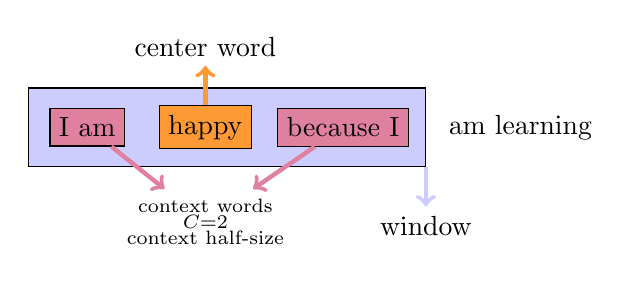
\begin{tikzpicture}
      \draw[fill=blue!20] (-2.75, -0.5) rectangle (2.3, 0.5);
      \node (window) at (2.3, -1.25) {window};
      \draw[->, ultra thick, blue!20] (2.3, -0.5) -- (window);
      \node[draw,fill=purple!50] (c1) at (-2,0) {I am};
      \node[draw,fill=orange!80] (center) at (-0.5,0) {happy};
      \node[draw,fill=purple!50] (c2) at (1.25,0) {because I};
      \node at (3.5, 0) {am learning};
      \node[below=5mm of center] (context) {$\substack{\textrm{context words} \\ C = 2 \\ \textrm{context half-size}}$};
      \draw[->, ultra thick, purple!50] (c1) -- (context);
      \draw[->, ultra thick, purple!50] (c2) -- (context);
      \node[above=5mm of center] (centerwordlabel) {center word};
      \draw[->, ultra thick, orange!80] (center) -- (centerwordlabel);
    \end{tikzpicture}
    \caption{In this example, the context words for the center word ``happy'' are ``I am'' and ``because I''. We define the \emph{window} as the count of the center word plus the context words; so, in this example the size of the window is equal to five.}
  \end{center}
\end{figure}

To train our model, we'll need a set of examples. Each example will be made of context words and the center word to be predicted. In the first example, the window is ``I am happy because I'', and the model will take the context words ``I am because I'', and should predict the center word ``happy''. We now slide the window by one word: the next training example that you have is ``am happy beause I am'', where the input to the model is the context words ``am happy I am'' and we want to predict the target center word ``because''. We continue to slide the window by one word again, and the model will take the window ``happy because I  am learning'', and we should predict ``I''.  This is described in detail in \href{https://arxiv.org/abs/1301.3781}{Efficient estimation of Word   Representations in Vector Space}. The model architecture is given by a shallow neural network:
\begin{figure}[h]
  \begin{center}
    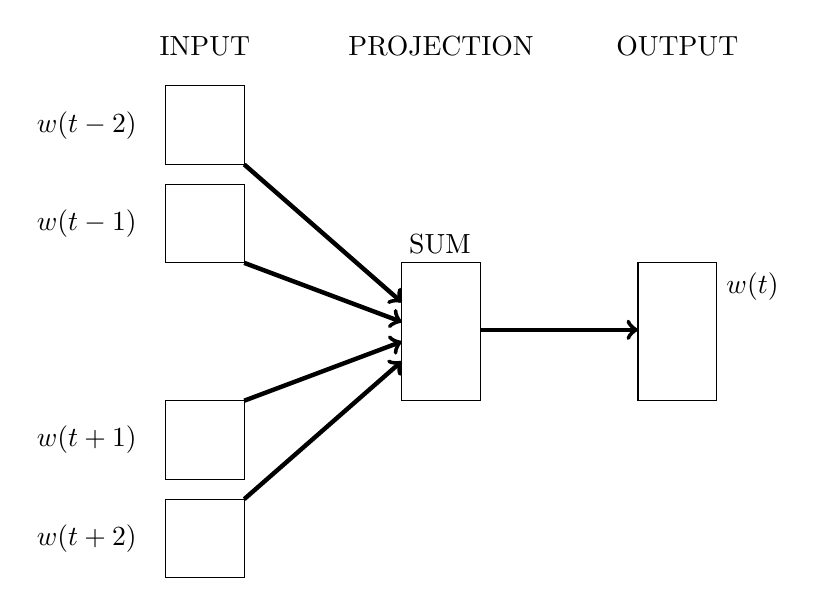
\begin{tikzpicture}
      \node at (-3, 3) {INPUT};
      \node (wtm2) at (-4.5, 2) {$w(t-2)$};
      \draw (-3.5, 1.5) rectangle (-2.5, 2.5);
      \node (wtm1) at (-4.5, 0.75) {$w(t-1)$};
      \draw (-3.5, 0.25) rectangle (-2.5, 1.25);
      \node (wtp1) at (-4.5, -2) {$w(t+1)$};
      \draw (-3.5, -2.5) rectangle (-2.5, -1.5);
      \node (wtp2) at (-4.5, -3.25) {$w(t+2)$};
      \draw (-3.5, -3.75) rectangle (-2.5, -2.75);
      \node at ( 0, 3) {PROJECTION};
      \draw (-0.5, -1.5) rectangle (+0.5, 0.25) node[above left] {SUM};
      \draw[->, ultra thick] (-2.5, 1.5) -- (-0.5, -0.25);
      \draw[->, ultra thick] (-2.5,0.25) -- (-0.5, -0.5);
      \draw[->, ultra thick] (-2.5,-1.5) -- (-0.5,-0.75);
      \draw[->, ultra thick] (-2.5,-2.75) -- (-0.5,-1);
      \node at (+3, 3) {OUTPUT};
      \draw (+2.5, -1.5) rectangle (+3.5, 0.25) node[below right] {$w(t)$};
      \draw[->, ultra thick] (0.5, -0.6) -- (2.5, -0.6);
    \end{tikzpicture}
  \end{center}
\end{figure}

\subsection{Cleaning and Tokenization} Let's go into more details on a fundamental technique for cleaning text data, in particular we'll discuss practical advice on how to clean a corpus and split it into words, or more accurately, tokens, through a process known as \emph{tokenization}.
\begin{enumerate}
\item Consider the words in our corpus as case insensitive, i.e. treat ``The'' identically no matter its casing/capitalization. This can be achieved by converting the entire corpus to either all lowercase or all uppercase.
\item Handle punctuation, which can be done in a variety of ways and which is suitable depends on the context. For example, we might choose to represent all interrupting punctuation marks (such as full stops, commas, and question marks) as a single special word of the vocabulary. You could choose to ignore non-interrupting punctuation marks such as quotation marks. You could also collapse multi-sign marks, such as triple question marks, into a single mark and so on.
\item You may want to handle numbers. E.g. if numbers don't carry an important meaning in your use case, you could drop all of the numbers. However, numbers may have significant meaning that is relevant to your use case. Examples include 3.14 (an approximation to $\pi$), 90210 (the name of a television show and the area code for Beverly Hills, CA). Therefore, one could argue towards keeping these numbers in the corpus as is. If your corpus has many unique numbers, e.g. many area codes, you may find that it makes more sense to replace all the numbers with a special token, such as \texttt{<NUMBER>}. This allows the model to know that the important thing is that it's a number, instead of trying to distinguish between numbers themselves.
\item Handle special characters, e.g. mathematical symbols, currency symbols, section and paragraph signs, and line markup signs etc. It's sometimes safe to drop these entirely.
\item Lastly, especially if working on a modern corpus of user inputs (e.g. tweets or user reviews), you should handle special words such as emojis and hashtags. Depending on if and how you want your model to confer meaning to them, you could, for example, consider that each emoji or hashtag be treated as an individual word.
\end{enumerate}

Consider as an example
``Who $\heartsuit$ "word embeddings" in 2020? I do!!!''.
This short tweet contains an emoji, punctuation, and a number.

\begin{python}
  # pip install nltk
  # pip install emoji
  import nltk
  from nltk.tokenize import word_tokenize
  import emoji

  nltk.download('punkt') # Download pre-trained Punkt tokenizer for English.

  # Use a regex to collapse all interrupting punctuation signs and replace them   with a full-stop.
  # Question mark and exclamation points replaced with single full-stop.
  data = re.sub(r'[,!?;-]+', '.', corpus)
  data = nltk.word_tokenize(data) # tokenize strings to words.
  data = [ ch.lower() for ch in data
           if ch.isalpha()
           or ch == '.'
           or emoji.get_emoji_regexp().search(ch)
         ]
\end{python}

\paragraph{Sliding window of words in Python} Suppose we've cleaned and tokenized the corpus and we now have an array of tokens or words. Let's now consider how to extract the center words and their context words, which will serve as examples to train the continuous bag of words model.

\begin{python}
def get_windows(words, C = 2):
  """ Words is a list of tokens."""  
  i = C
  while i < len(words) - C:
    center_word = words[i];
    context_words = words[(i-C):i] + words[(i+1):(i+C+1)]
    yield context_words, center_word
    i += 1
\end{python}

Notice this is a \emph{generator} function; with a \emph{yield} we can pause execution of the function until the next time it is invoked.

\paragraph{Transforming words into vectors} At this point, we've cleaned and tokenized our corpus and extracted the context words and center word from a window that slides across our prepared corpus. We're now ready to transform the center words and context words into a mathematical form that's going to be consumed by the continuous bag of words model. Let's start with the center word: for the sample corpus
\begin{verbatim}
I am happy because I'm learning
\end{verbatim}
we first create a vocabulary, which is the set of unique words in the corpus $V = \{\textrm{am, because, happy, I, learning}\}$. We can now encode each word as a column one-hot vector, just like in section \ref{par: onehotvectors}. In this way, the vector for ``am'' will have a unit value in the row corresponding to ``am'' and a zero everywhere else, for example.
For the context words, we'll create a \emph{single} vector that represents the average of individual one-hot vectors. E.g.

\begin{equation*}
  \frac{1}{4} \times 
  \begin{bmatrix}
    & \textrm{I} & & \textrm{am} & & \textrm{because} & & \textrm{I} & \\
    \textrm{am} & {\color{blue!50} 0} & & {\color{blue!50}1} & & {\color{blue!50}0} & & {\color{blue!50}0} & \\
    \textrm{because} & {\color{blue!50}0} & & {\color{blue!50}0} & & {\color{blue!50}1} & & {\color{blue!50}0} & \\
    \textrm{happy} & {\color{blue!50}0} & + & {\color{blue!50}0} & + & {\color{blue!50}0} & + & {\color{blue!50}0} \\
    \textrm{I} & {\color{blue!50}1} & & {\color{blue!50}0} & & {\color{blue!50}0} & & {\color{blue!50}1} & \\
    \textrm{learning} & {\color{blue!50}0} & & {\color{blue!50}0} & & {\color{blue!50}0} & & {\color{blue!50}0} &
\end{bmatrix}
= \begin{bmatrix} \textrm{I am because I} \\
  0.25 \\
  0.25 \\
  0 \\
  0.5 \\
  0
\end{bmatrix}
\end{equation*}
So, if we repeat this process for our vocabular, we come up with the following inputs for our ML algorithm.
\begin{table}[h]
  \begin{center}
    \begin{tabular}{c c c c}
      \hline
      Context words & Context words vector & Center word & Center word vector \\
      \hline
      I am because I & $\begin{bmatrix} 0.25; 0.25; 0; 0.5; 0 \end{bmatrix}$ &                                                                                                                                                                                                                                                                                                                                                                                                                                                                                                                                                                          happy & $\begin{bmatrix} 0; 0; 1; 0; 0 \end{bmatrix}$ \\
      am happy I am & $\begin{bmatrix} 0.5; 0; 0.25; 0.25; 0 \end{bmatrix}$ &                                                                                                                                                                                                                                                                                                                                                                                                                                                                                                                                                                                                                                                        because & $\begin{bmatrix} 0; 1; 0; 0; 0 \end{bmatrix}$ \\
      happy because am learning & $\begin{bmatrix} 0.25; 0.25; 0.25; 0, 0.25 \end{bmatrix}$ &                                                                                                                                                                                                                                                                                                                                                                                                                                                                                                                                                                                                                                  I & $\begin{bmatrix} 0; 0; 0; 1; 0 \end{bmatrix}$ \\
    \end{tabular}
  \end{center}
\end{table}

\paragraph{Architecture of the CBOW model} The continuous bag of words model is based on a shallow, dense neural network with an input layer, a single hidden layer, and an output layer. The input to the model is a vector of context words, which we'll call $X$, and the output is the vector of the predicted center word $\hat y$.

\begin{figure}[h]
  \begin{center}
    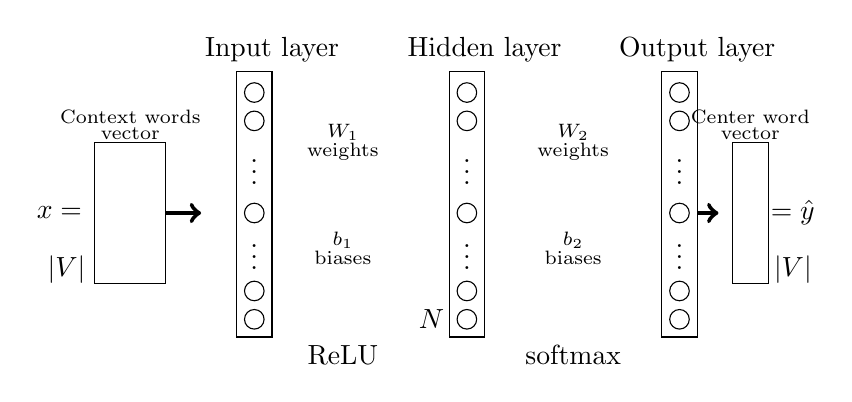
\begin{tikzpicture}[scale=0.9]
      % Context words vector (i.e. raw input)
      \draw (-2, 1) rectangle (-1, 3);
      \node at (-1.5, 3.25) {$\substack{\textrm{Context words} \\           \textrm{vector}}$};
      \node at (-2.5, 2) {$x = $};
      \node at (-2.4, 1.2) {$|V|$};
      \draw[->, ultra thick] (-1, 2) -- (-0.5, 2);
      % Input layer.
      \draw (0, 0.25) rectangle (0.5, 4) node[above] {Input layer};
      \node[draw,circle,scale=0.75] at (0.25, 0.5) {};
      \node[draw,circle,scale=0.75] at (0.25, 0.9) {};
      \node at (0.25, 2.7) {$\vdots$};
      \node[draw,circle,scale=0.75] at (0.25, 2) {};
      \node at (0.25, 1.5) {$\vdots$};
      \node[draw,circle,scale=0.75] at (0.25, 3.3) {};
      \node[draw,circle,scale=0.75] at (0.25, 3.7) {};
      % First weights matrix and bias layer.
      \node at (1.5, 3) {$\substack{W_1 \\ \textrm{weights}}$};
      \node at (1.5, 1.5) {$\substack{b_1 \\ \textrm{biases}}$};
      \node at (1.5, 0) {ReLU};
      % Hidden layer.
      \draw (3, 0.25) rectangle (3.5, 4) node[above] {Hidden layer};
      \node[draw,circle,scale=0.75] at (3.25, 0.5) {};
      \node[draw,circle,scale=0.75] at (3.25, 0.9) {};
      \node at (3.25, 2.7) {$\vdots$};
      \node[draw,circle,scale=0.75] at (3.25, 2) {};
      \node at (3.25, 1.5) {$\vdots$};
      \node[draw,circle,scale=0.75] at (3.25, 3.3) {};
      \node[draw,circle,scale=0.75] at (3.25, 3.7) {};
      \node at (2.75, 0.5) {$N$};
      % Second weights matrix and bias layer.
      \node at (4.75, 3) {$\substack{W_2 \\ \textrm{weights}}$};
      \node at (4.75, 1.5) {$\substack{b_2 \\ \textrm{biases}}$};
      \node at (4.75, 0) {softmax};
      % Output layer.
      \draw (6, 0.25) rectangle (6.5, 4) node[above] {Output layer};
      \node[draw,circle,scale=0.75] at (6.25, 0.5) {};
      \node[draw,circle,scale=0.75] at (6.25, 0.9) {};
      \node at (6.25, 2.7) {$\vdots$};
      \node[draw,circle,scale=0.75] at (6.25, 2) {};
      \node at (6.25, 1.5) {$\vdots$};
      \node[draw,circle,scale=0.75] at (6.25, 3.3) {};
      \node[draw,circle,scale=0.75] at (6.25, 3.7) {};
      % Center word vector
      \draw[->, ultra thick] (6.5, 2) -- (6.8, 2);
      \draw (7, 1) rectangle (7.5, 3);
      \node at (7.25, 3.25) {$\substack{\textrm{Center word} \\                     \textrm{vector}}$};
\node at (7.85, 1.2) {$|V|$};
\node at (7.85, 2) {$= \hat y$};
\end{tikzpicture}
\caption{\small In this neural network, the size of the input and output vectors is the size of the vocabulary, $|V|$. If you recall from the previous section on word embedding process, the size or dimension of the word embeddings is a hyperparameter we select. This hidden layer is related to our embedding, and its size is a hyperparameter $N$; in practice $N$ is in the range of hundreds to thousands. We're going to use a regular feed-forward neural network, i.e. a dense neural network with fully connected layers. Our algorithm will learn weights matrices $W_i$ and bias terms $b_i$ as we train it. For the input-to-hidden layer, we'll use a Rectified Linear Unit activation function, whereas for the output layer we'll use a softmax.}
  \end{center}
\end{figure}

\paragraph{Dimensions of the CBOW model architecture}
Let's be clear on the dimensions of our vectors and matrices in our neural network diagram.

\begin{itemize}
\item Our input layer is of dimension $|V| \times 1$.
\item To get the values in the hidden layer, we first calculate $z_1 = W_1 x + b_1$. Then, we compute the activation $h = \texttt{ReLU}(z_1)$. In terms of dimensions, $W_1$ is $N \times |V|$, where $N$ is the size of the word embeddings. $b_1$ is of dimension $N \times 1$. The hidden layer is therefore of dimension $N \times 1$, since $z_1$ is an $N \times 1$ column vector and \texttt{ReLU} is applied element-wise.
\item To get the values of the output layer, we need to calculate (i) the weighted sum from the hidden layer plus the bias term $z_2 = W_2 h + b_2$, and then apply the activation function $\hat y = \texttt{softmax}(z_2)$. Notice that $W_2$ is of dimension $|V| \times N$, and $b_2$ is of length $|V|$. When we compute $z_2$, it's a vector of length $|V|$, and when we pass it through the softmax we get back a vector of length $|V|$.
\end{itemize}

\paragraph{Vectorized implementation} What if instead of passing a single training example through our neural network, we wanted to pass through several examples at a time. This makes the learning process quicker and is known as \emph{batch processing}. Say you want to feed $m$ input context word vectors into the neural network during each iteration; $m$ is called the batch size and is a hyperparameter for the model that we define at training time. We can prepare a data matrix $X$ where the $m$ column vectors of length $|V|$ represent words: we get a data matrix of dimension $|V| \times m$.

\begin{figure}[h]
  \begin{center}
    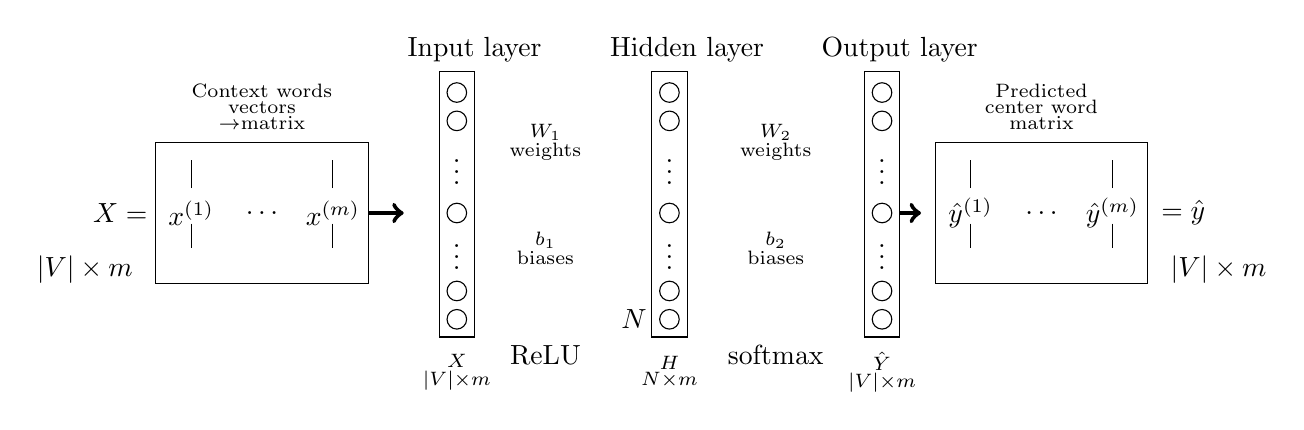
\begin{tikzpicture}[scale=0.9]
      % Context words matrix (i.e. raw input)
      \draw (-4, 1) rectangle (-1, 3);
      \node at (-2.5, 3.5) {$\substack{\textrm{Context words} \\           \textrm{vectors} \\ \rightarrow \textrm{matrix}}$};
      \node at (-4.5, 2) {$X = $};
      \draw (-3.5, 2.35) -- (-3.5, 2.75);
      \node at (-3.5, 2) {$x^{(1)}$};
      \draw (-3.5, 1.85) -- (-3.5, 1.5);
      \node at (-2.5, 2) {$\ldots$};
      \draw (-1.5, 2.35) -- (-1.5, 2.75);
      \node at (-1.5, 2) {$x^{(m)}$};
      \draw (-1.5, 1.85) -- (-1.5, 1.5);
      \node at (-5, 1.2) {$|V| \times m$};
      \draw[->, ultra thick] (-1, 2) -- (-0.5, 2);
      % Input layer.
      \draw (0, 0.25) rectangle (0.5, 4) node[above] {Input layer};
      \node[draw,circle,scale=0.75] at (0.25, 0.5) {};
      \node[draw,circle,scale=0.75] at (0.25, 0.9) {};
      \node at (0.25, 2.7) {$\vdots$};
      \node[draw,circle,scale=0.75] at (0.25, 2) {};
      \node at (0.25, 1.5) {$\vdots$};
      \node[draw,circle,scale=0.75] at (0.25, 3.3) {};
      \node[draw,circle,scale=0.75] at (0.25, 3.7) {};
      \node at (0.25, -0.25) {$\substack{X \\ |V| \times m}$};
      % First weights matrix and bias layer.
      \node at (1.5, 3) {$\substack{W_1 \\ \textrm{weights}}$};
      \node at (1.5, 1.5) {$\substack{b_1 \\ \textrm{biases}}$};
      \node at (1.5, 0) {ReLU};
      % Hidden layer.
      \draw (3, 0.25) rectangle (3.5, 4) node[above] {Hidden layer};
      \node[draw,circle,scale=0.75] at (3.25, 0.5) {};
      \node[draw,circle,scale=0.75] at (3.25, 0.9) {};
      \node at (3.25, 2.7) {$\vdots$};
      \node[draw,circle,scale=0.75] at (3.25, 2) {};
      \node at (3.25, 1.5) {$\vdots$};
      \node[draw,circle,scale=0.75] at (3.25, 3.3) {};
      \node[draw,circle,scale=0.75] at (3.25, 3.7) {};
      \node at (2.75, 0.5) {$N$};
      \node at (3.25, -0.25) {$\substack{H \\ N \times m}$};
      % Second weights matrix and bias layer.
      \node at (4.75, 3) {$\substack{W_2 \\ \textrm{weights}}$};
      \node at (4.75, 1.5) {$\substack{b_2 \\ \textrm{biases}}$};
      \node at (4.75, 0) {softmax};
      % Output layer.
      \draw (6, 0.25) rectangle (6.5, 4) node[above] {Output layer};
      \node[draw,circle,scale=0.75] at (6.25, 0.5) {};
      \node[draw,circle,scale=0.75] at (6.25, 0.9) {};
      \node at (6.25, 2.7) {$\vdots$};
      \node[draw,circle,scale=0.75] at (6.25, 2) {};
      \node at (6.25, 1.5) {$\vdots$};
      \node[draw,circle,scale=0.75] at (6.25, 3.3) {};
      \node[draw,circle,scale=0.75] at (6.25, 3.7) {};
      \node at (6.25, -0.25) {$\substack{\hat Y \\ |V| \times m}$};
      % Center word matrix
      \draw[->, ultra thick] (6.5, 2) -- (6.8, 2);
      \draw (7, 1) rectangle (10, 3);
      \node at (8.5, 3.5) {$\substack{\textrm{Predicted} \\ \textrm{center word} \\                     \textrm{matrix}}$};
      \draw (7.5, 2.35) -- (7.5, 2.75);
      \node at (7.5, 2) {$\hat y^{(1)}$};
      \draw (7.5, 1.85) -- (7.5, 1.5);
      \node at (8.5, 2) {$\ldots$};
      \draw (9.5, 2.35) -- (9.5, 2.75);
      \node at (9.5, 2) {$\hat y^{(m)}$};
      \draw (9.5, 1.85) -- (9.5, 1.5);
      \node at (11, 1.2) {$|V| \times m$};
      \node at (10.5, 2) {$= \hat y$};
\end{tikzpicture}
\caption{\small When batch processing data, our input becomes a matrix $X$ where the columns are the representations for context words; the input matrix is of dimension $|V| \times m$, since we have $m$ examples and we're using a one-hot encoding for our initial word representation. We then calculate $Z_1 = W_1 X + B_1$ where now $B_1$ is an $N \times m$ matrix of $m$ \emph{identical} $b_1$ bias vectors, each of length $N$; note that we can perform \emph{broadcasting} in Python to add a vector to a matrix and the desired result is achieved. We continue with calculating elementwise $H = \texttt{ReLU}(Z_1)$. Next, we compute $\hat Y$, via $Z_2 = W_2 H + B$ followed by $\hat Y = \texttt{softmax}(Z_2)$. We finally see that $\hat Y$ is of dimension $|V| \times m$: i.e. we have $m$ column vectors, where each one corresponds to a predicted center word. Essentially, the first column of the input matrix is transformed into the first column of the output matrix, and similarly for the remaining $m-1$ input vectors.}
  \end{center}
\end{figure}

\paragraph{Activation functions} Let's first discuss \texttt{ReLU}, or rectified linear unit, then we'll get into \texttt{softmax}. Excepting input neurons, which are used ``as-is'', each layer first calculates the weighted sum of its inputs, adds a bias, and then passes the result into an activation function. I.e. for the first hidden layer we calculate $z_1 = W_1 x + b_1$, and to get $h$, we feed $z_1$ through the activation function $h = \texttt{ReLU}(z_1)$. ReLU is a popular general purpose activation function that only activates the neuron if the sum of its weighted input is positive. Mathematically, we have that $\texttt{ReLU}(x) = \max(0, x)$. We can plot the function:


\begin{figure}[h]
  \centering   
  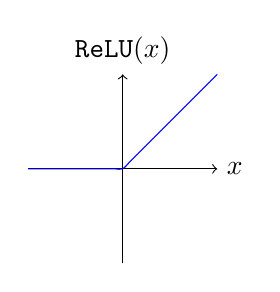
\begin{tikzpicture}[scale=1.2]
    \draw[->] (-1,0) -- (1,0) node[right] {$x$};   
    \draw[->] (0,-1) -- (0,1) node[above] {$\texttt{ReLU}(x)$};
    \draw[domain=-1:1,smooth,variable=\x,blue] plot ({\x},{max(0,\x)}); 
  \end{tikzpicture}
  \caption{A plot of the ReLU function.}
\end{figure}

E.g., $\texttt{ReLU}(\begin{bmatrix} 5.1 & -0.3 & \ldots & -4.6 & 0.2 \end{bmatrix} = \begin{bmatrix} 5.1 & 0 & \ldots & 0 & 0.2 \end{bmatrix}$. Now, for the output layer we'll calculate the weighted sum of the values from the hidden layer and add the bias vector, i.e. $z = W_2 h + b_2$, and then we pass this through the activation function $\texttt{softmax}(z) = \hat y$. The \emph{softmax} function takes in a vector $z \in \mathbb R^k$ and outputs a vector $[0,1]^k$ where the result is a probabilitiy distribution, i.e. $\sum = 1$. When we apply softmax to $z$, the result is that we get a probability distribution over the words in the corpus.

\begin{table}[h]
  \begin{center}
    \begin{tabular}{c c c |l}
      $z$ & & $\hat y$  & $\substack{\textrm{Probabilities} \\ \textrm{of being} \\ \textrm{center word}}$\\
      \hline
      $z_1$ & & $\hat y_1$ & a \\
      $\vdots$ & & $\vdots$  & $\vdots$ \\
      $z_i$ & $\overset{\texttt{softmax}}{\longrightarrow}$ & $\hat y_i$ & happy \\
      $\vdots$ & & $\vdots$ & $\vdots$ \\
      $z_{|V|}$ & & $\hat y_{|V|}$ & zebra
    \end{tabular}
    \caption{The softmax function takes in a vector of real numbers $z \in \mathbb R^k$, as opposed to \texttt{ReLU} which operates on scalars. The output of softmax is a vector of real numbers in the interval $[0,1]$ which sum to 1 and can be interpreted as probabilities of exclusive events. In the case of a continuous bag of words model, when you apply softmax to $z$, you obtain an output vector $\hat y$ with $|V|$ rows, where each row corresponds to a word of the vocabulary of the corpus. The values of the vector can be interpreted as the probability that the center word which is what the model is trying to predict is the word that is assigned to each of the rows.}
  \end{center}
\end{table}

Mathematically,
\[
  \hat y_i = \frac{e^{z_i}}{\sum_j e^{z_j}}.
\]
The exponential transforms all inputs to positive real numbers, and the denominator normalizes the value to lie in the unit interval.

\paragraph{Cost function for softmax} In order to predict one of the $|V|$ possible words, we need to minimize a certain cost function.

\begin{figure}[h]
  \begin{center}
    \begin{tikzpicture}
      % Input.
      \node[draw,fill=purple!20] (input) at (-4, 0) {Input};
      \node[above=2mm of input] {$\substack{\textrm{Context} \\ \textrm{words}           \\ \textrm{vector}}$};
      \draw[->, ultra thick] (input) -- (-1.3, 0);
      % CBOW
      \node (mlmodel) at (0, 0) {$\substack{\textrm{Machine learning} \\                     \textrm{model}}$};
      \node[above=2mm of mlmodel] {CBOW};
      \node[draw,fill=green!20] (params) at (0, -1)       {$\substack{\textrm{Parameters} \\ W_1, b_1, W_2, b_2}$};
      \draw (-1.25 , -1.5) rectangle (1.25, 0.5);
      % Predictions and Truth.
      \node[draw,fill=orange!20,right=8mm of mlmodel] (prediction) {Prediction};
      \node[above=2mm of prediction] {$\substack{\hat y \\ \textrm{Predicted} \\ \textrm{center word} \\ \textrm{vector}}$};
      \node[draw,fill=purple!20,right=3mm of prediction] (truth) {Truth};
      \node[above=2mm of truth] {$\substack{y \\ \textrm{Actual} \\           \textrm{center word} \\ \textrm{vector}}$};
      \path[draw,decorate,decoration={brace,amplitude=10pt,mirror}] (1.9, -0.5)       -- (5.9, -0.5);
      \node[draw,fill=green!20] (loss) at (3.85, -1.3) {loss};
      \node[right=2mm of loss] {error};
      \node[below=2mm of loss] {cross-entropy loss};
      % Relationship
      \draw[->] (1, -1) -- (loss) node[midway,above,rotate=-5] {minimize};
      \draw[->] (3.4, -1.5) -- (params) node[midway,below,rotate=-5] {adjust};
    \end{tikzpicture}
  \end{center}
\end{figure}

The formula for cross-entropy loss is given by
\[
  J = -\sum_{k=1}^{|V|} y_k \log \hat y_k.
\]

Let's look at a quick example, the corpus ``I am happy because I am learning'' with context ``I am because I'' and target word ``happy'' (window is ``I am happy because I'').

\begin{table}[h]
  \begin{center}
    \begin{tabular}{c | l c c c}
      $y$ & & $\hat y$ & $\log \hat y$ & $y \odot \log \hat y$ \\
      \hline
      0 & am & 0.083 & -2.49 & 0 \\
      0 & because & 0.03 & -3.49 & 0 \\
      \textbf{1} & \textbf{happy} & \textbf{0.611} & -0.49 & -0.49 \\
      0 & I & 0.225 & -1.49 & 0 \\
      0 & learning & 0.05 & -2.49 & 0
    \end{tabular}
    \caption{In this case, we predicted the correct target word and so the loss was $J = 0.49$.}
  \end{center}
\end{table}

More generally, $J = - \log \hat y_{\texttt{actual word}}$.

\begin{figure}[h]
  \begin{center}
    \begin{tikzpicture}[scale=1]
      \draw[->] (0,0) -- (2.5,0) node[right] {$\hat y_{\texttt{actual word}}$};   
      \draw[->] (0,0) -- (0,3) node[above] {$\texttt{cross-entropy loss}(x)$};
      \draw[domain=0.1:2,smooth,variable=\x,blue] plot ({\x},-{ln(\x)}+0.75);
      \node at (2.5, 0.75) {\color{green!80!black} $\substack{\textrm{correct} \\ \textrm{predictions} \\ \textrm{reward}}$};
      \node at (1.2, 2) {\color{purple!80} $\substack{\textrm{incorrect} \\ \textrm{predictions} \\ \textrm{penalty}}$};
    \end{tikzpicture}
    \caption{As you can see, in our simplified cost function, the model is penalizing incorrect predictions by incurring a high cost, and giving correct predictions a reward by incurring a lower cost.}
  \end{center}
\end{figure}

\subsubsection{Training a CBOW model}
\paragraph{Forward propagation} asdf

\end{document}



